\chapter{Saliency and Attribution Methods}\label{ch:saliency}

This chapter develops interpretability methods from the streams $g,h$ with $f=g-h$ constructed in Section~\ref{sec:dc_splitting_relu}. Section~\ref{sec:split_attribution_concept} reads the streams separately to explain pretrained networks through SplitCAM, SplitLRP and SplitGrad~\parencite{hiddenMono}. It also studies directly trained difference-of-convex input neural networks (DCINNs), whose MNIST examples exhibit class-dependent stream sensitivities. Section~\ref{sec:game_based_attribution} collects practical \emph{modes} that turn the game equilibria of Chapter~\ref{ch:game_theory} into tunable attribution maps, and the \emph{technicalities} of equivariant averaging that improve attribution quality.

\section{Split-Based and Difference-of-Convex Attribution}\label{sec:split_attribution_concept}

Post-hoc attribution assigns each input feature a score for its influence on a fixed network output. Established families include gradient saliency~\parencite{Simonyan2014}, deconvolution and guided backpropagation~\parencite{ZeilerFergus2014,Springenberg2015}, \ac{lrp} and deep Taylor decomposition~\parencite{Bach2015,Montavon2017DeepTaylor}, class-activation mapping~\parencite{Zhou2016,Selvaraju2017}, baseline-based methods such as Integrated Gradients and DeepLIFT~\parencite{Sundararajan2017,Shrikumar2017}, noise-averaged gradients~\parencite{Smilkov2017}, and perturbation- or surrogate-based explanations~\parencite{Ribeiro2016,FongVedaldi2017,LundbergLee2017,Kolek2023_ShearletX,Fel2023_EVA}. These explain the original network. We identify signal loss in rules using ordinary local derivatives, then develop SplitCAM, SplitLRP and SplitGrad from the separate signals preserved by the split-pair of Section~\ref{sec:dc_splitting_relu}, closing with by-design DCINNs.

PRCA and DRSA optimize relevance over activation subspaces; their virtual layer preserves the decision function when a full orthogonal basis is retained~\parencite{Chormai2024DRSA}. Our split representation separates contributions using the original network's signs and gates.

Consider a feedforward \ac{relu} network with layers $1,\dots,L$, weights $\Wl{l}$, pre-activations $\preactl{l}=\Wl{l}\actl{l-1}$, hidden activations $\actl{l}=\relu(\preactl{l})$ for $l<L$, and ungated readout $\actl{L}=\preactl{L}$. We attribute a fixed scalar class logit: $f^{(l)}\colon\RR^{d^{(l)}}\to\RR$ denotes layers $l+1,\dots,L$ acting on layer-$l$ activations. Biases are absorbed as in Section~\ref{sec:dc_splitting_relu}. The split streams $g^{(l)},h^{(l)}\colon\RR^{d^{(l)}}\times\RR^{d^{(l)}}\to\RR$ act on $\act{l}{+},\act{l}{-}$ and satisfy
\begin{equation}
	f^{(l)}\bigl(a^{+} - a^{-}\bigr) = g^{(l)}(a^{+}, a^{-}) - h^{(l)}(a^{+}, a^{-})
	\qquad \text{for all } a^{+}, a^{-} \in \RR^{d^{(l)}},
	\label{eq:split_correctness_recall}
\end{equation}
and we write $g\coloneqq g^{(0)}$, $h\coloneqq h^{(0)}$ with balanced input split $\act{0}{\pm}=\pm x/2$. Derivatives are row vectors (scalar Jacobians); derivative statements hold at differentiability points, hence Lebesgue-almost everywhere because all functions involved are \ac{cpwl}.

A \ac{relu} gate transmits positive pre-activations and otherwise returns zero, erasing their negative magnitude and blocking the local gradient. This \emph{subthreshold signal loss} hides the suppressed pre-activation from the output through that gate and from backward rules retaining its ordinary derivative. Ordinary input gradients can therefore exhibit exact regional blindness.

\begin{proposition}[Regional blindness of the input gradient, \LeanResult{prop:gradient_blindness}]\label{prop:gradient_blindness}
Let $f$ be as above and $x_0$ an input with no zero pre-activations. If every path from input coordinate $i$ to the output passes through a neuron inactive at $x_0$, then $\partial f/\partial x_i\equiv0$ on some open neighborhood $U\ni x_0$, even if $f$ depends on $x_i$ elsewhere.\end{proposition}

\begin{proof}
Set $M^{(l,+)}\coloneqq\diag\bigl(\1\{\preactl{l}>0\}\bigr)$, $M^{(l,-)}\coloneqq\diag\bigl(\1\{\preactl{l}\leq0\}\bigr)$ and $\Wl{l,x}\coloneqq M^{(l,+)}\Wl{l}$ for hidden layers $1\leq l<L$. The affine logit readout is ungated and may be negative, so $\Wl{L,x}\coloneqq\Wl{L}=\partial f/\partial\actl{L-1}$. Continuity and nonzero hidden pre-activations at $x_0$ give an open $U\ni x_0$ with constant masks and affine $f$. Iterating the chain rule on $U$ yields
\begin{equation}
	\frac{\partial f}{\partial x}
	= \Wl{L,x} \, \Wl{L-1,x} \cdots \Wl{1,x},
	\label{eq:masked_path_product}
\end{equation}
and its $i$-th entry sums weight products over paths from input $i$ to the output, multiplied by indicators that every hidden neuron on the path is active; the output carries no mask. Every path contains an inactive hidden neuron, so every summand vanishes throughout $U$.
\end{proof}

The phenomenon already occurs in a single-hidden-neuron network.

\begin{remark}[The canonical counterexample]\label{rem:sensitivity_counterexample}
Following \textcite{Sundararajan2017}, consider the one-dimensional \ac{relu} network
\begin{equation}
	f(x) = 1 - \relu(1 - x),
	\label{eq:ig_counterexample}
\end{equation}
and compare input $x=2$ with baseline $x'=0$. The prediction changes by $f(2)-f(0)=1$, making the sole feature relevant. Yet $f$ is constant on $x\geq1$: at $x=2$, gradients, Input$\times$Gradient and rules retaining local \ac{relu} derivatives assign zero attribution. The hidden neuron is inactive, so Proposition~\ref{prop:gradient_blindness} applies with $U=(1,\infty)$.
\end{remark}

\textcite{Sundararajan2017} axiomatize this requirement.

\begin{definition}[Sensitivity(a)]\label{def:sensitivity}
An attribution method $A$, mapping an input $x$ and a baseline $x'$ to feature scores $A_i(x, x') \in \RR$, satisfies \emph{Sensitivity} if for every pair $(x, x')$ that differs in exactly one feature $i$ and satisfies $f(x) \neq f(x')$, the attribution of that feature is non-zero, $A_i(x, x') \neq 0$.
\end{definition}

Plain gradients violate Sensitivity (Remark~\ref{rem:sensitivity_counterexample}). Integrated Gradients restores it by integrating the gradient along the segment from $x'$ to $x$, requiring many forward--backward passes and inheriting the baseline choice. The split-pair instead preserves subthreshold signals in the \emph{representation} used for attribution.

Recall from Section~\ref{sec:dc_splitting_relu} how the split-pair processes a \ac{relu} gate: the pre-activation pair $\preact{l}{+}, \preact{l}{-}$ is mapped to
\begin{equation}
	\act{l}{+} = \max\bigl\{\preact{l}{+}, \preact{l}{-}\bigr\},
	\qquad
	\act{l}{-} = \preact{l}{-},
	\label{eq:split_maxout_gate}
\end{equation}
a rank-2 Maxout unit in the $g$-stream and identity in the $h$-stream. Their difference reproduces $\relu(\preactl{l})$. At an inactive neuron, both activations equal $\preact{l}{-}$: the suppressed signal's magnitude remains in their common level. The backward pass likewise retains subthreshold information.

\begin{definition}[Local sensitivities]\label{def:local_sensitivities}
Use the row sensitivities $\delta^{(l,\sigma,s)}$ of \eqref{eq:local_sensitivities}, for $s\in\{g,h\}$, $\sigma\in\{+,-\}$ and $0\le l\le L$, and write $\delta^{(l)}\coloneqq\partial f^{(l)}/\partial\actl{l}$. Abbreviate the absolute-weight product \eqref{eq:w_abs} by $W_{\mathrm{abs}}^{[l]}$, with $W_{\mathrm{abs}}^{[L]}=\1^\top$. For our scalar output, its $i$-th entry sums absolute weight products over all paths from layer-$l$ neuron $i$ to the output, active or inactive.
\end{definition}

The four local sensitivities obey coupled backward recursions, the split analogue of backpropagation underlying this chapter's methods.

\begin{lemmaenv}[Split backward recursions, \LeanResult{lem:split_backward_recursion}]\label{lem:split_backward_recursion}
With the activation masks $M^{(l,\pm)}$ of Proposition~\ref{prop:gradient_blindness}, extended by $M^{(L,+)}=I$ and $M^{(L,-)}=0$ for the affine readout, for every $0 \leq l < L$ and $s \in \{g, h\}$,
\begin{align}
	\delta^{(l, +, s)}
	&= \delta^{(l+1, +, s)} \bigl( M^{(l+1, +)} \Wsig{l+1}{+} + M^{(l+1, -)} \Wsig{l+1}{-} \bigr)
	+ \delta^{(l+1, -, s)} \, \Wsig{l+1}{-},
	\label{eq:delta_plus_recursion} \\
	\delta^{(l, -, s)}
	&= \delta^{(l+1, +, s)} \bigl( M^{(l+1, +)} \Wsig{l+1}{-} + M^{(l+1, -)} \Wsig{l+1}{+} \bigr)
	+ \delta^{(l+1, -, s)} \, \Wsig{l+1}{+},
	\label{eq:delta_minus_recursion}
\end{align}
with base case $\delta^{(L, +, g)} = \delta^{(L, -, h)} = \1^{\top}$ and $\delta^{(L, -, g)} = \delta^{(L, +, h)} = 0$.\end{lemmaenv}

The block Jacobians \eqref{eq:split_layer_jacobians} give these recursions: the maximum selects $\preact{l+1}{+}$ exactly at active neurons. Adding the recursions eliminates the complementary masks.

\begin{proposition}[Sensitivity mass conservation, \LeanResult{prop:sensitivity_mass}]\label{prop:sensitivity_mass}
For every $0 \leq l \leq L$ and both streams $s \in \{g, h\}$,
\begin{equation}
	\delta^{(l, +, s)} + \delta^{(l, -, s)} = W_{\mathrm{abs}}^{[l]}.
	\label{eq:mass_conservation}
\end{equation}\end{proposition}

\begin{proof}
Write $S^{(l)}=\delta^{(l,+,s)}+\delta^{(l,-,s)}$. Adding \eqref{eq:delta_plus_recursion} and \eqref{eq:delta_minus_recursion} gives $S^{(l)}=S^{(l+1)}|\Wl{l+1}|$, since $M^{(l+1,+)}+M^{(l+1,-)}=I$ and $\Wsig{l+1}{+}+\Wsig{l+1}{-}=|\Wl{l+1}|$. Backward induction from $S^{(L)}=\1^\top$ yields $S^{(l)}=W_{\mathrm{abs}}^{[l]}$.
\end{proof}

Differentiating split correctness recovers the original gradient.

\begin{corollary}[Backward invariant, \LeanResult{cor:backward_invariant}]\label{cor:backward_invariant}
For every $0 \leq l \leq L$,
\begin{equation}
	\delta^{(l, +, g)} - \delta^{(l, +, h)} = \delta^{(l)} = -\bigl( \delta^{(l, -, g)} - \delta^{(l, -, h)} \bigr),
	\quad \text{hence} \quad
	\bigl( \delta^{(l,+,g)} - \delta^{(l,-,g)} \bigr) - \bigl( \delta^{(l,+,h)} - \delta^{(l,-,h)} \bigr) = 2\,\delta^{(l)}.
	\label{eq:backward_invariant}
\end{equation}\end{corollary}

\begin{proof}
Differentiate the correctness identity \eqref{eq:split_correctness_recall} with respect to $a^{+}$ and $a^{-}$, respectively, and subtract the two resulting identities.
\end{proof}

For the combined gradients \eqref{eq:unified_split_gradients}, Corollary~\ref{cor:backward_invariant} gives $\delta^{(l,g)}-\delta^{(l,h)}=\delta^{(l)}$: regional blindness means equal combined stream gradients, possibly both zero. Partial sensitivities can differ from $\tfrac12W_{\mathrm{abs}}^{[l]}$, recording routing at active and inactive \ac{relu} gates. Proposition~\ref{prop:sensitivity_mass} guarantees a positive partial sensitivity per head for each feature connected to the output by a nonzero-weight path, without guaranteeing nonzero partial differences, combined gradients or attribution. For example, with $f(x)=\relu(\relu(x)+\relu(-x)-10)$ and balanced input split, both heads equal $10$ locally near $x=1$, and both combined gradients vanish.

\begin{remark}[The counterexample, revisited]\label{rem:counterexample_split}
For \eqref{eq:ig_counterexample} with balanced split $\act{0}{\pm}=\pm x/2$, Section~\ref{sec:dc_splitting_relu} gives $g(x)=x/2+1$, $h(x)=x/2$ and $g(x)-h(x)=1=f(x)$ for $x>1$. At $x=2$ both stream gradients equal $\tfrac{1}{2}$, while $f'(2)=\tfrac{1}{2}-\tfrac{1}{2}=0$. Thus the heads supply a nonzero signal consistent with $f(2)\neq f(0)$, even where their difference is constant. This example with $x'=0$ does not establish Definition~\ref{def:sensitivity} for arbitrary attribution rules or baselines. The following methods turn the pair-valued signal into scalar maps; the shifted combinations of Section~\ref{sec:split_grad} avoid exact cancellation here and assign positive attribution for every $\alpha<\tfrac{1}{2}$.
\end{remark}

Non-negative weights let each neuron only \emph{add} evidence, a structure long associated with interpretability~\parencite{ayinde2018nonnegativity,lee1999nmf}. The split-pair gives an arbitrary pretrained network this structure by doubling its width; the following methods exploit its signal flow.

\subsection{SplitCAM}\label{sec:split_cam}

\ac{cam} methods explain \ac{cnn} decisions by combining spatial activation maps of a convolutional layer with class-specific weighting coefficients. The original \ac{cam}~\parencite{Zhou2016} requires a global-average-pooling head; Grad-CAM~\parencite{Selvaraju2017} extends it to \acp{cnn} without that head requirement by weighting each channel with the spatially pooled gradient of the class logit, and Grad-CAM++~\parencite{Chattopadhay2018} refines the pooling weights. LayerCAM~\parencite{Jiang2021LayerCAM} drops the pooling altogether and weights every spatial location individually: for a layer $l$ with channel activation maps $\actl{l}_c$ and class logit $y$,
\begin{equation}
	\text{LayerCAM}^{(l)} = \relu\Bigl( \sum_{c} \relu\!\Bigl(\frac{\partial y}{\partial \actl{l}_c}\Bigr) \odot \actl{l}_c \Bigr),
	\label{eq:layercam}
\end{equation}
where $\odot$ denotes the elementwise product and the sum runs over the channels. This makes LayerCAM applicable to early layers with high spatial resolution. Inactive neurons contribute no activation-weighted term, and the positive-gradient weighting discards negative gradient evidence.

\emph{SplitCAM} applies LayerCAM's spatial activation weighting to signed split-stream maps. Raw sensitivities sum \emph{absolute} path products (Proposition~\ref{prop:sensitivity_mass}) and become numerically enormous in deep split-pairs, requiring the stabilized sensitivities of Section~\ref{subsec:backward_stabilization}.

\begin{definition}[Shifted local sensitivities, \LeanResult{def:shifted_sensitivities}]\label{def:shifted_sensitivities}
Fix shift parameters $\alpha^{(l)} \in [0, \tfrac{1}{2}]$. For $s \in \{g, h\}$ define, backward from layer $L$, intermediate sensitivities $\delta_{\mathrm{int}}^{(l, \pm, s)}$ by evaluating the recursions \eqref{eq:delta_plus_recursion}--\eqref{eq:delta_minus_recursion} (respectively the base case of Lemma~\ref{lem:split_backward_recursion} at $l = L$) with the already-shifted sensitivities of the subsequent layer, and set
\begin{equation}
	\delta_{\mathrm{shift}}^{(l, \pm, s)}
	\coloneqq \delta_{\mathrm{int}}^{(l, \pm, s)} - \alpha^{(l)} \bigl( \delta_{\mathrm{int}}^{(l, +, s)} + \delta_{\mathrm{int}}^{(l, -, s)} \bigr),
	\qquad
	\delta_{\mathrm{shift}}^{(l, s)} \coloneqq \frac{\delta_{\mathrm{shift}}^{(l, +, s)} - \delta_{\mathrm{shift}}^{(l, -, s)}}{2}.
	\label{eq:shift_definition}
\end{equation}
\end{definition}

The common shift preserves sensitivity differences. By \eqref{eq:claim_bulk}, its intermediate bulk is $\delta_{\mathrm{int}}^{(l,+,s)}+\delta_{\mathrm{int}}^{(l,-,s)}=\bigl[\prod_{i=l+1}^L(1-2\alpha^{(i)})\bigr]W_{\mathrm{abs}}^{[l]}$, with empty product $1$; the factor $\tfrac12$ matches the balanced input split \eqref{eq:unified_split_gradients}. We use $\alpha^{(l)}\equiv\alpha$ unless stated otherwise. Theorem~\ref{thm:closed_formula_shift} gives raw sensitivities at $\alpha=0$, multiples of the original gradient at $\alpha=\tfrac12$, and controlled layer-dependent damping of the split signal for $0<\alpha<\tfrac12$.

\paragraph{The SplitCAM attribution.}\label{subsec:splitcam_definition}
\begin{definition}[SplitCAM]\label{def:splitcam}
For a layer $l$ of the decomposed model, a stream $s \in \{g, h\}$ and a sign $\sigma \in \{+, -\}$, the SplitCAM attribution maps are
\begin{align}
	\text{SplitCAM}^{(l, \sigma, s)} &\coloneqq \sum_{c} \delta_{\mathrm{shift}}^{(l, \sigma, s)}\big\vert_c \odot \act{l}{\sigma}_c,
	\label{eq:splitcam_stream} \\
	\text{SplitCAM}^{(l, s)} &\coloneqq \sum_{c} \delta_{\mathrm{shift}}^{(l, s)}\big\vert_c \odot \actl{l}_c,
	\label{eq:splitcam_combined}
\end{align}
where $\act{l}{\sigma}_c$ denotes the channel-$c$ activation map of the $\sigma$-stream, $\actl{l}_c = \act{l}{+}_c - \act{l}{-}_c$ the reconstructed original activation map, and $\cdot\vert_c$ the restriction of a sensitivity tensor to channel $c$.
\end{definition}

SplitCAM \emph{omits positive-gradient clipping and the outer $\relu$}, retaining signed shifted sensitivities. It uses shifted sensitivities rather than raw derivatives: \eqref{eq:shift_definition} changes each map only by multiples of the pattern-independent $W_{\mathrm{abs}}^{[l]}$, keeping the quantities numerically meaningful.

Under Section~\ref{sec:stabilization_dc}, the forward pass scales split activations and restores their invariant against cached original activations. The backward pass applies Definition~\ref{def:shifted_sensitivities} using masks from those activations, preserving \eqref{eq:backward_invariant} against the cached original gradient.

\paragraph{Layer choice and resolution.}
Like LayerCAM, SplitCAM is defined at every layer, and the resulting map is bilinearly upsampled to the input resolution. Empirically the method peaks in the deep convolutional blocks --- for VGG-16~\parencite{Simonyan2015} at layer 26 --- where it concentrates on entire classified objects noticeably better than LayerCAM at the same layer; the full layer-ablation study and the quantitative comparison on the Quantus benchmark~\parencite{Hedstrom2023} for VGG-16 and ResNet-18~\parencite{He2016resnet} are reported in Chapter~\ref{ch:experiments}.

\subsection{SplitLRP}\label{sec:split_lrp}

\ac{lrp}~\parencite{Bach2015} propagates a relevance budget backward, distributing each neuron's relevance to its inputs in proportion to their contributions; \textcite{Montavon2018} give an overview and \textcite{Kohlbrenner2020} best practices. The $\gamma$-rule~\parencite{Montavon_2022_gammaLRP} emphasizes positive contributions. We use its bias-excluding, $\varepsilon$-stabilized variant: for $\preactl{l+1}_i=\sum_j\Wl{l+1}_{ij}\actl{l}_j+b^{(l+1)}_i$, define
\begin{equation}
	\tilde{z}^{(l+1)}_{ij} \coloneqq \actl{l}_j \Bigl( \Wl{l+1}_{ij} + \gamma\, \posneg{\Wl{l+1}_{ij}}{+} \Bigr),
	\qquad \gamma \geq 0,
	\label{eq:gamma_contribution}
\end{equation}
and redistributes the relevances $R^{(l+1)}_i$ onto the inputs as
\begin{equation}
	R^{(l)}_j = \sum_i \frac{\tilde{z}^{(l+1)}_{ij}}{\sum_{j'} \tilde{z}^{(l+1)}_{ij'} + \varepsilon \, \operatorname{sign}\bigl( \sum_{j'} \tilde{z}^{(l+1)}_{ij'} \bigr)} \, R^{(l+1)}_i,
	\label{eq:lrp_gamma_rule}
\end{equation}
with a small stabilizer $\varepsilon > 0$. Setting $\gamma = 0$ gives the corresponding bias-excluding $\varepsilon$-rule. For affine--ReLU blocks, ReLU activations pass relevance through unchanged, and redistribution acts on the affine layers.

\paragraph{Relevance propagation on the split-pair.}\label{subsec:splitlrp_definition}
\emph{SplitLRP} treats both streams as neuron groups in one decomposed network. Each layer carries relevance tensors $R^{(l,+)},R^{(l,-)}$, jointly propagated through the four coupling blocks built from $\Wsig{l}{+},\Wsig{l}{-}$. Propagation starts at the class-specific positive $g$-output $\act{L}{+}$. All weights are non-negative, so we use \eqref{eq:lrp_gamma_rule} with $\gamma=0$, $\varepsilon=10^{-6}$: the $\varepsilon$-rule needs no preference for positive over negative contributions. Paired Maxout gates \eqref{eq:split_maxout_gate} are transparent in the relevance pass.

The following conventions complete the specification.
\begin{itemize}
	\item \emph{Forward pass.} The split activations are computed with the same scaling stabilization and forward-invariant correction of Section~\ref{sec:stabilization_dc} as SplitCAM.
	\item \emph{Normalization.} The denominator of \eqref{eq:lrp_gamma_rule} renormalizes relevance layer-wise, preserving the combined budget of $R^{(l,+)},R^{(l,-)}$ at $\act{L}{+}$ up to the $\varepsilon$-stabilizer (Remark~\ref{rem:splitlrp_markov}). This replaces backward shifting (Definition~\ref{def:shifted_sensitivities}).
	\item \emph{Pooling and normalization layers.} Relevance passes through max-pooling by the winner-takes-it-all scheme, assigning the full relevance to the location attaining the maximum; batch-nor\-mal\-iza\-tion layers are merged into the adjacent linear or convolutional layers beforehand; residual additions split relevance evenly across branches.
\end{itemize}

\begin{definition}[Combined SplitLRP map]\label{def:splitlrp_combined}
The SplitLRP attribution at layer $l$ is the pair $\bigl(R^{(l,+)}, R^{(l,-)}\bigr)$; the \emph{combined} map is
\begin{equation}
	R^{(l, \mathrm{comb})} \coloneqq R^{(l, +)} - R^{(l, -)}.
	\label{eq:splitlrp_combined}
\end{equation}
\end{definition}

Positive-stream relevance traverses an even number of sign inversions and represents support; negative-stream relevance represents opposition. Equation~\eqref{eq:splitlrp_combined} combines them into a signed saliency map.

\begin{remark}[A probabilistic reading]\label{rem:splitlrp_markov}
The original network's $\varepsilon$-rule mixes signed contributions, producing a signed path measure (Chapter~\ref{ch:trajectory}). In the split-pair, $\tilde{z}^{(l+1)}_{ij}$ multiplies non-negative activations and weights. Up to the stabilizer, its propagation matrices are stochastic: SplitLRP is a Markov chain on the doubled graph, with unsigned relevance measure $\bigl(R^{(l,+)},R^{(l,-)}\bigr)$. Doubling the state space absorbs weight signs, as in the stopping game's probabilistic backward flow (Chapter~\ref{ch:game_theory}).
\end{remark}

\begin{remark}[Sensitivity to learned parameters]\label{rem:splitlrp_sanity}
The parameter-randomization sanity check of \textcite{Adebayo2018sanity} differentiates the three split methods. After reinitializing the last three feedforward layers of VGG-16, every reported SplitCAM and SplitGrad configuration has lower SSIM than every listed baseline, whereas the HOG and Spearman comparisons are mixed. This establishes sensitivity to the tested parameter changes, not faithfulness to the learned decision process. SplitLRP retains high HOG and Spearman similarity despite a decrease in SSIM. This retained structure is consistent with parameter-insensitivity concerns for some relevance-propagation rules~\parencite{sixt2020whenexplanationslie}, but the comparison does not identify the mechanism in SplitLRP. Section~\ref{app:p1_sanity} reports the quantitative results and the caveats of \textcite{Binder2022shortcomings} on randomization-based checks.
\end{remark}

\subsection{SplitGrad}\label{sec:split_grad}

SplitGrad uses the stabilized combined gradients of \eqref{eq:unified_split_gradients} directly. The balanced embedding $\act{0}{\pm}=\pm x/2$ gives the factor $\tfrac12$ in \eqref{eq:shift_definition}; Theorem~\ref{thm:closed_formula_shift} shows that the difference of the stabilized sensitivities of the two convex heads recovers the exact original gradient.

\begin{definition}[SplitGrad]\label{def:splitgrad}
For a layer $l$ and stream $s \in \{g, h\}$, the SplitGrad attribution map is the channel mean of the combined shifted sensitivity,
\begin{equation}
	\text{SplitGrad}^{(l, s)} \coloneqq \frac{1}{C^{(l)}} \sum_{c = 1}^{C^{(l)}} \delta_{\mathrm{shift}}^{(l, s)}\big\vert_c,
	\label{eq:splitgrad}
\end{equation}
where $C^{(l)}$ is the number of channels of layer $l$; the default configuration reads the $g$-stream, with forward and backward stabilization exactly as in Section~\ref{sec:split_cam}.
\end{definition}

\paragraph{What SplitGrad measures.}\label{subsec:closed_formulas}
Theorem~\ref{thm:closed_formula_shift} gives original-gradient terms $\delta/2$ and $-\delta/2$, where $\delta=\partial f/\partial x$, minus a shared, geometrically damped sum of layer-wise \emph{subthreshold probe-gradients} through inactive neurons. The shared sum cancels in the difference, recovering $\delta$. It can itself vanish, so subthreshold contributions need not yield nonzero attribution. In Remark~\ref{rem:counterexample_split}, however, $\delta=0$ and the probe term is nonzero, correctly attributing the feature for every $\alpha<\tfrac12$. The factors $\overline\alpha_j$ counteract probe-gradient growth toward the input, interpolating between full split information ($\alpha=0$) and signed halves of the original gradient ($\alpha=\tfrac12$). The sweep in Chapter~\ref{ch:experiments} supports metric- and configuration-dependent choices: the two main-text configurations have localization optima at $\alpha=0.35$ or $0.4$, and lowest Maximum Sensitivity at $\alpha=0$ (full ablation: Section~\ref{app:ablation}).

The three methods share one pipeline: a stabilized split forward pass caching the original activations, a stabilized backward pass --- relevance-based for SplitLRP (initialized at the class-specific $\act{L}{+}$ and propagated by the $\varepsilon$-rule), sensitivity-based otherwise (the shifted recursions of \eqref{eq:shift_definition}) --- and a method-specific readout, with the resulting map bilinearly upsampled to the input resolution. The network can be split once per model. In the reported implementation, SplitCAM takes approximately 14--29 times as long per image as the corresponding ordinary Grad-CAM and LayerCAM configurations; SplitGrad also takes substantially longer. Their timings are of the same order as the row labeled Guided Grad-CAM, but the released VGG-16 configuration dispatches Guided LayerCAM, limiting identification of that baseline. Section~\ref{app:p1_timing} details this ambiguity and the measurement scope.


\subsection{Directly Trained Difference-of-Convex Input Neural Networks}\label{sec:dcinns}

To study mechanisms exposed by the \ac{dc} decomposition of pretrained networks (Sections~\ref{sec:split_cam}--\ref{sec:split_grad}), we directly train small DC input neural networks (DCINNs) and their monotone relatives on MNIST. Their shared opposing-stream structure provides a controlled setting for examining class-dependent sensitivities on present and candidate missing strokes, with a modest, architecture-dependent accuracy cost.

\paragraph{Architecture and training.}\label{subsec:dcinn_architecture}

Use the \ac{icnn} and monotone-network definitions from Section~\ref{sec:convex_monotone_foundations}. An \ac{icnn}~\parencite{Amos2017} is a convex, monotone network acting on an unconstrained affine first layer (Definition~\ref{def:icnn}); constraining that layer too gives monotonicity in the original input (Propositions~\ref{prop:icnn_convex} and~\ref{prop:monotone_represents}).

\begin{definition}[DCINN and difference-of-monotone models]\label{def:dcinn}
For a fixed base architecture, a \emph{DCINN} (DIC model) is $f_{\mathrm{DIC}}=g-h$, where $g,h$ are independently parameterized \acp{icnn}, trained jointly by empirical risk minimization on their difference. A \emph{DM model} instead uses two monotone networks. The \emph{inverted-input} variants DICIN and DMIN feed $h$ the complement $\1-x$ for inputs in $[0,1]^d$.
\end{definition}

The two non-negative streams learn convex (respectively monotone) functions, making their difference a training-time inductive bias. Related CDiNN architectures address optimal control~\parencite{Sankaranarayanan2021CDINN}, with recurrent extensions for safety-critical model predictive control~\parencite{Chen2025_RCDiNN}; we study interpretability. Feeding a monotone $h$-stream $\1-x$ makes it accumulate evidence from missing input mass.

Three implementation choices matter in practice.
\begin{itemize}
	\item \emph{Activations.} Both streams use convex, monotone rank-2 Maxout units~\parencite{Goodfellow2013Maxout}, which consistently outperformed \ac{relu} streams in the difference setting. Their constrained layers use the same non-negative-weight Maxout building blocks as the split-stream construction in Section~\ref{sec:dc_splitting_relu}.
	\item \emph{Non-negativity.} Constrained weights are parameterized as $p(\tilde{W})$ with free parameters $\tilde{W}$ and a positivity transform $p$; among softplus, exponential and squaring, $p = \relu$ with absolute-value-of-Gaussian initialization gave the best test accuracy. The transform is also applied to biases and to the scale and shift parameters of batch-normalization layers.
	\item \emph{Regularization.} Since non-negative weights preclude cancellation, activations can grow quickly; a small initialization scale and a weight decay of $10^{-3}$ keep the streams stable during training.
\end{itemize}

The empirical study uses two MNIST base architectures: \texttt{cnn\_maxout}, a \ac{cnn} with four convolutional layers (32, 64, 128 and 128 channels with batch normalization) followed by three fully connected layers, roughly $1.2$ million parameters in total, and \texttt{mlp\_maxout}, a wide four-layer \ac{mlp} ($784 \to 800 \to 800 \to 800 \to 10$) with roughly $4.2$ million parameters --- each in eight variants: unconstrained (None), single-stream constrained (IC, Mon), and difference-of-two models (DIC, DM, DICIN, DMIN, and an unconstrained difference baseline).

\paragraph{Stream sensitivities and candidate counterfactual features.}\label{subsec:counterfactual_features}

The directly trained streams expose \emph{plain input gradients} without shifting, relevance rules or probe networks. For an inverted-input DIC class logit $f(x)=g(x)-h(\1-x)$, $\nabla g(x)$ measures the sensitivity of $g(x)$, while $(\nabla h)(\1-x)$ measures that of $-h(\1-x)$ to increases in the original input: complement and subtraction cancel the two chain-rule signs. At differentiable inputs, the complete model gradient is
\begin{equation*}
	\nabla f(x)=\nabla g(x)+(\nabla h)(\1-x).
\end{equation*}
The first affine layer of an \ac{icnn} is unconstrained, so convexity of the streams does not make either gradient non-negative in the original input coordinates. A positive entry of one stream gradient can be outweighed by a negative entry of the other. Even a positive entry of the complete gradient only establishes an increase for sufficiently small feasible increases in that coordinate at a differentiable input; it does not establish a necessary feature or a change in the predicted class. Finite counterfactual claims require evaluating the complete model under the proposed intervention. The displayed maps are thus stream-local sensitivities; their concentration on present and candidate missing strokes motivates a factual/counterfactual interpretation to be tested by interventions.

\begin{figure}[t]
\QualitativeImageContent{
	\centering
	\begin{minipage}[c]{0.15\linewidth}
		\centering
		
\includegraphics[width=\linewidth]{saliency/mnist_split_ic_saliency/image_030_true_3_pred_3/original.png}\\[-1pt]
		{\scriptsize Original}
	\end{minipage}\hspace{0.015\linewidth}%
	\begin{minipage}[c]{0.80\linewidth}
		\centering
		\begin{minipage}[b]{0.19\linewidth}\centering
			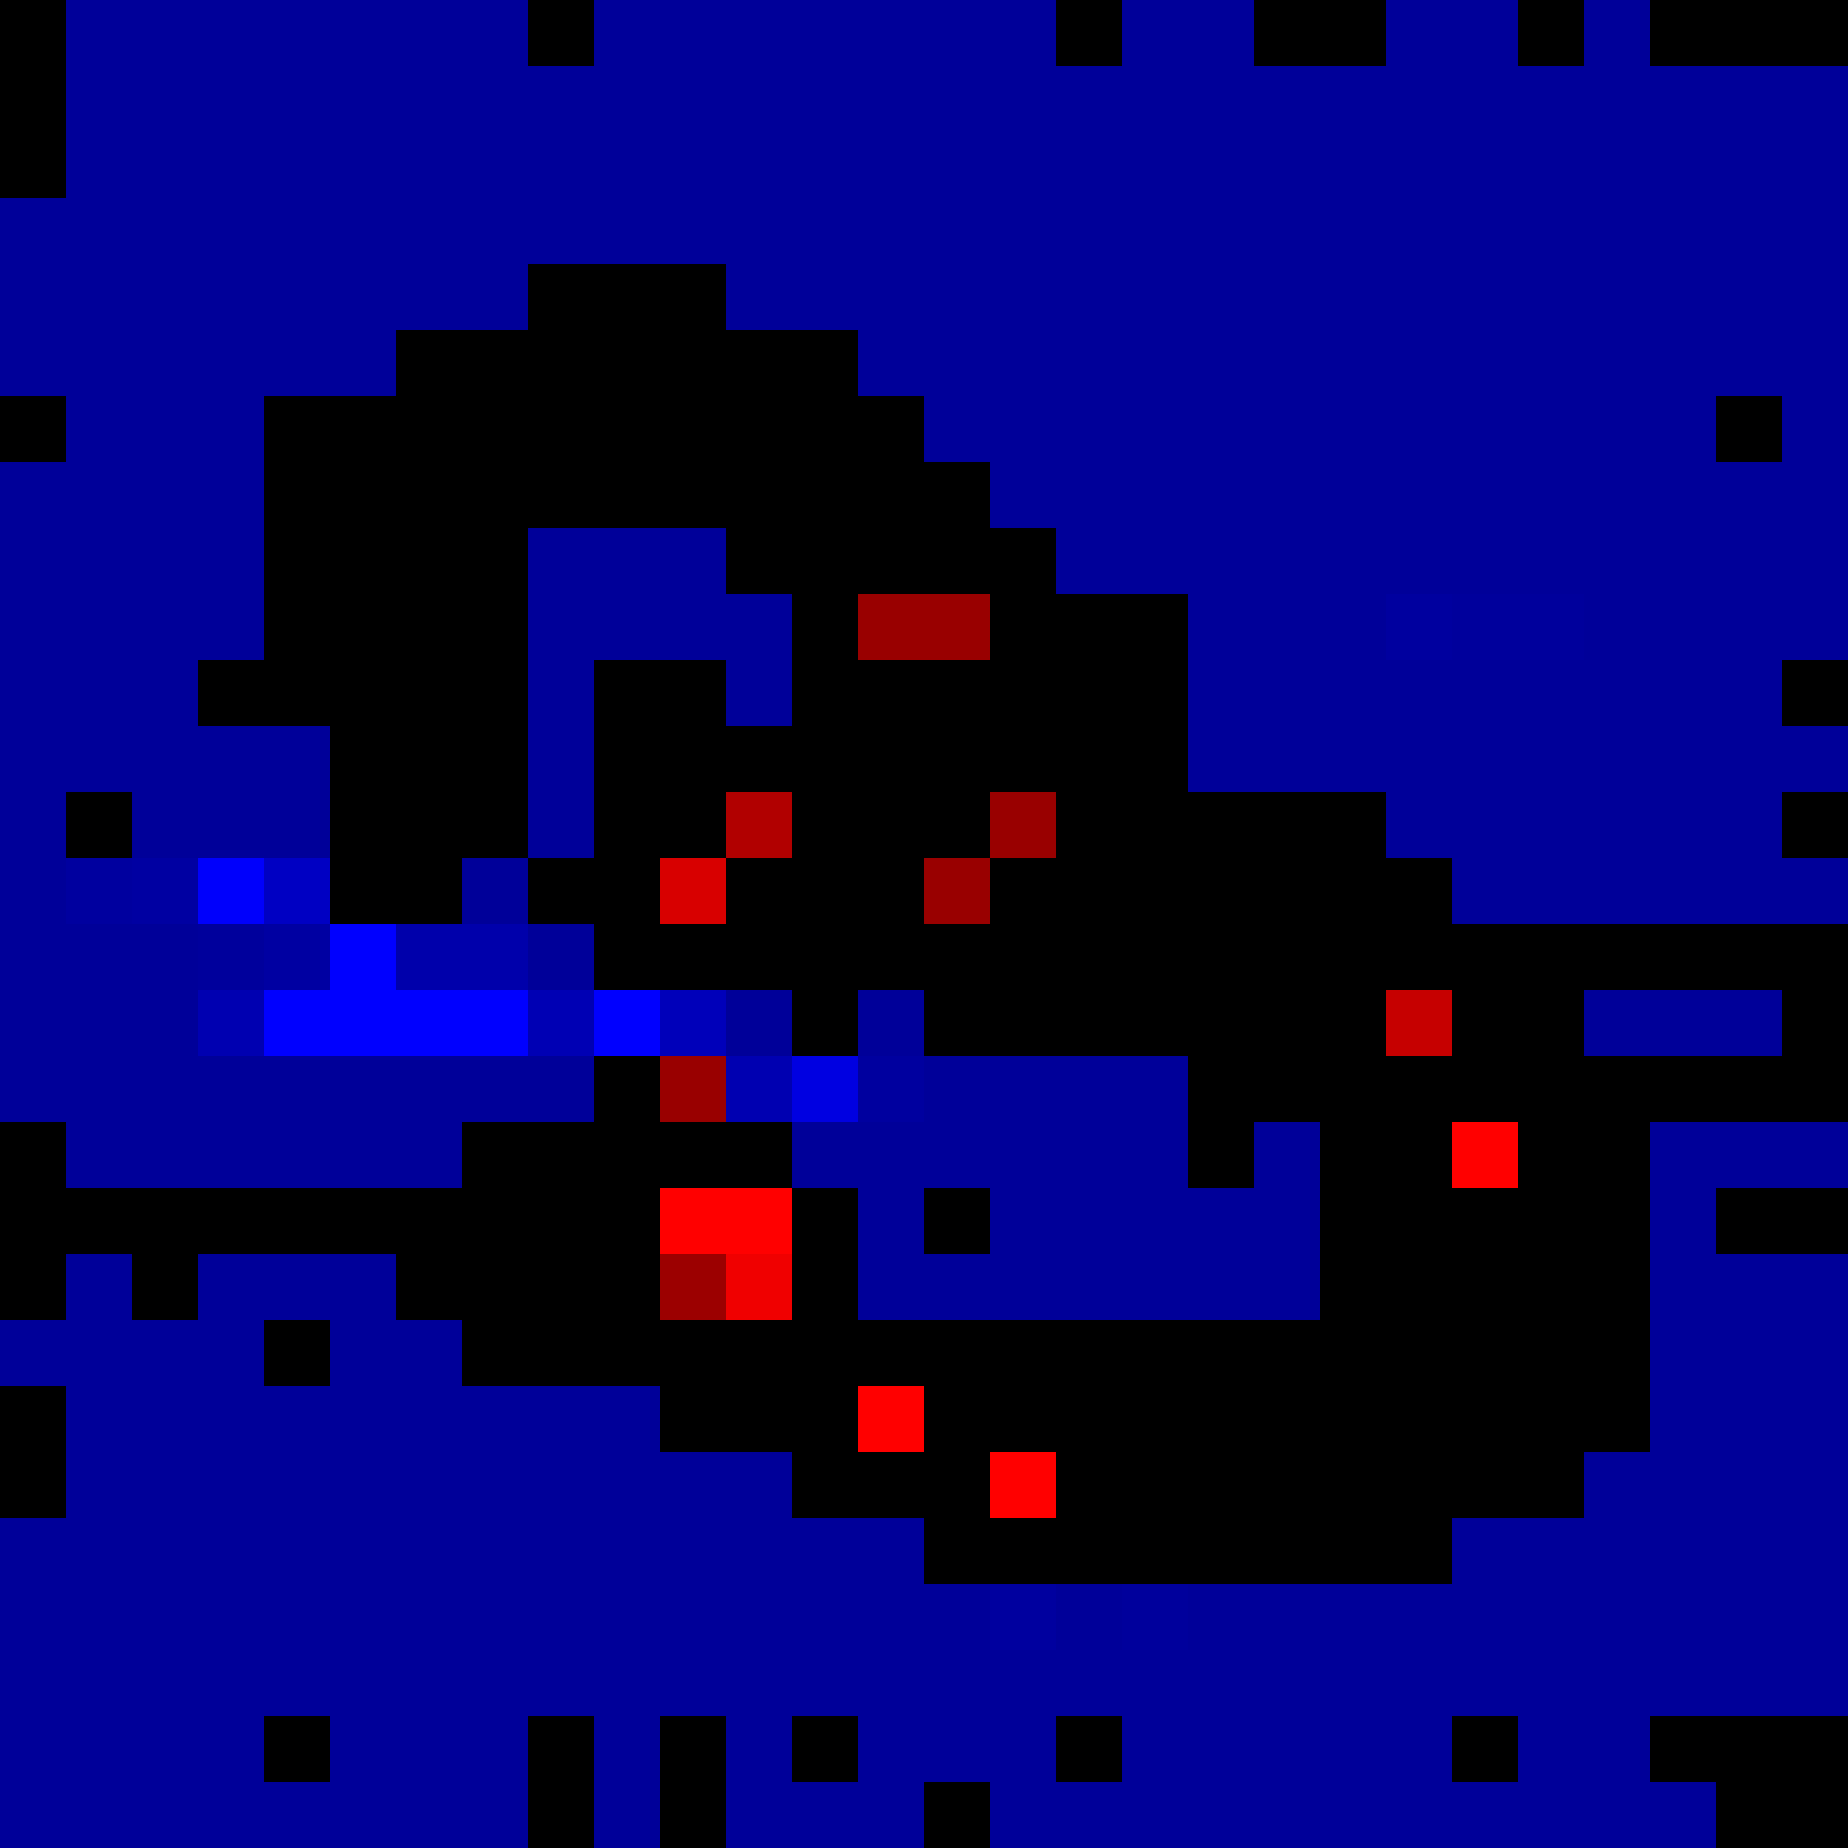
\includegraphics[width=\linewidth]{saliency/mnist_split_ic_saliency/image_030_true_3_pred_3/final_saliency_threshold_wrt_0_bright.png}\\[-1pt]{\scriptsize Logit 0}
		\end{minipage}%
		\begin{minipage}[b]{0.19\linewidth}\centering
			
\includegraphics[width=\linewidth]{saliency/mnist_split_ic_saliency/image_030_true_3_pred_3/final_saliency_threshold_wrt_1_bright.png}\\[-1pt]{\scriptsize Logit 1}
		\end{minipage}%
		\begin{minipage}[b]{0.19\linewidth}\centering
			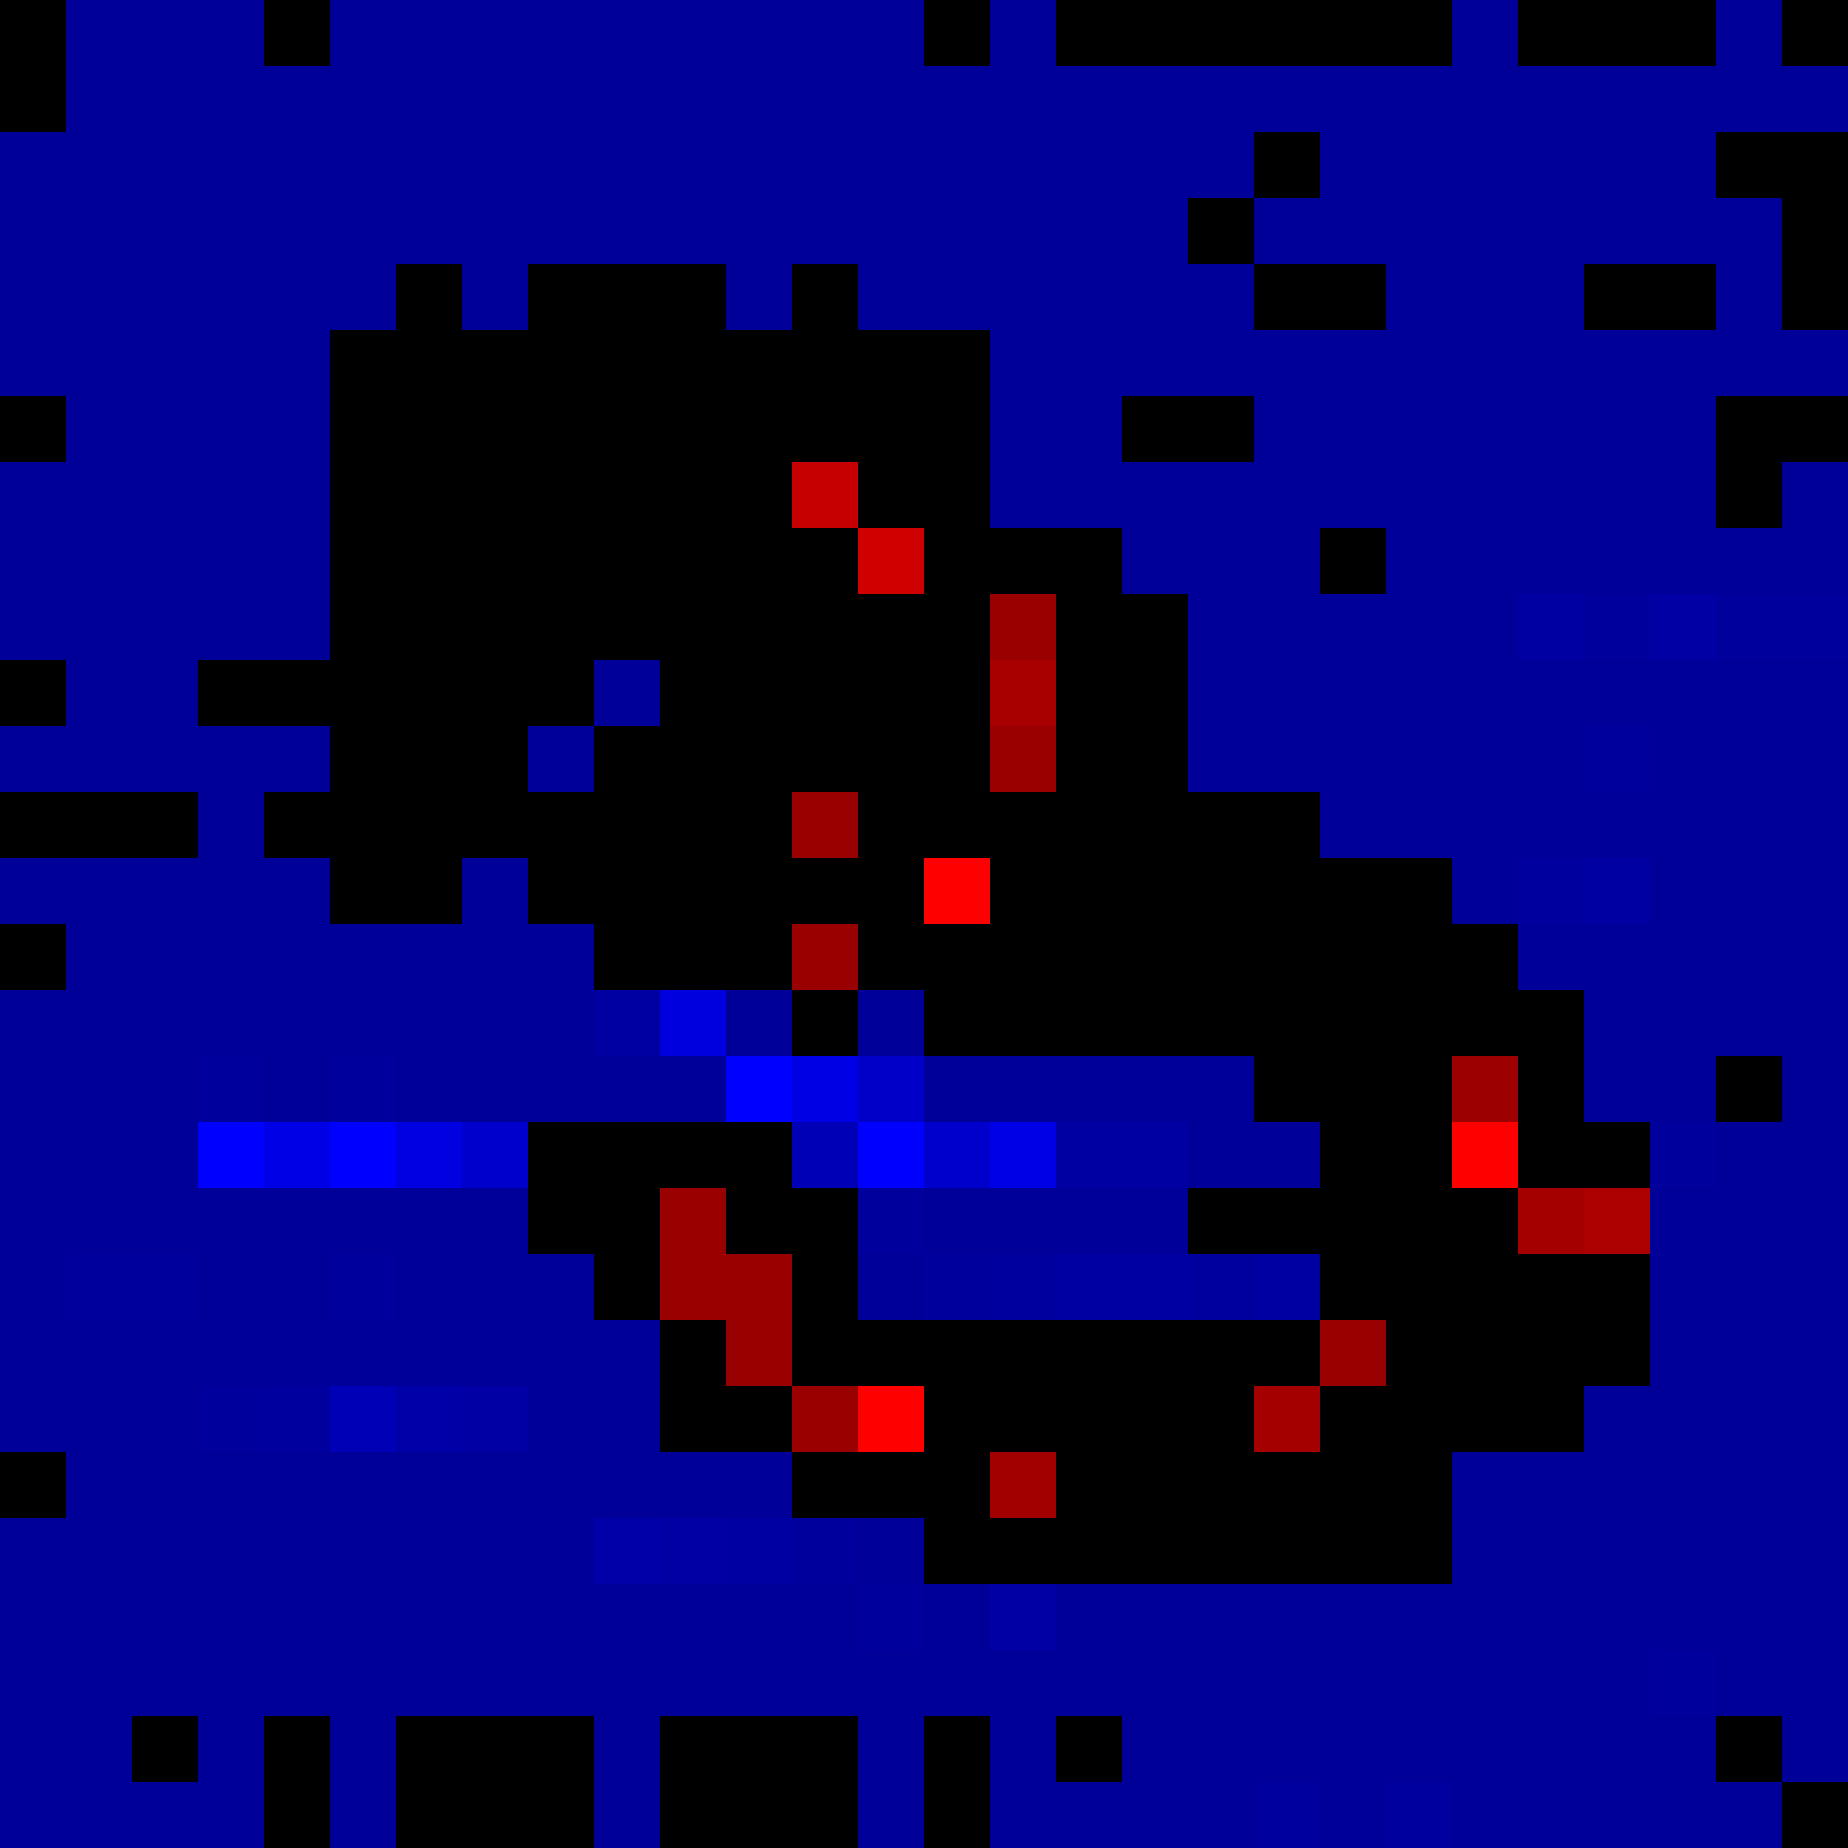
\includegraphics[width=\linewidth]{saliency/mnist_split_ic_saliency/image_030_true_3_pred_3/final_saliency_threshold_wrt_2_bright.png}\\[-1pt]{\scriptsize Logit 2}
		\end{minipage}%
		\begin{minipage}[b]{0.19\linewidth}\centering
			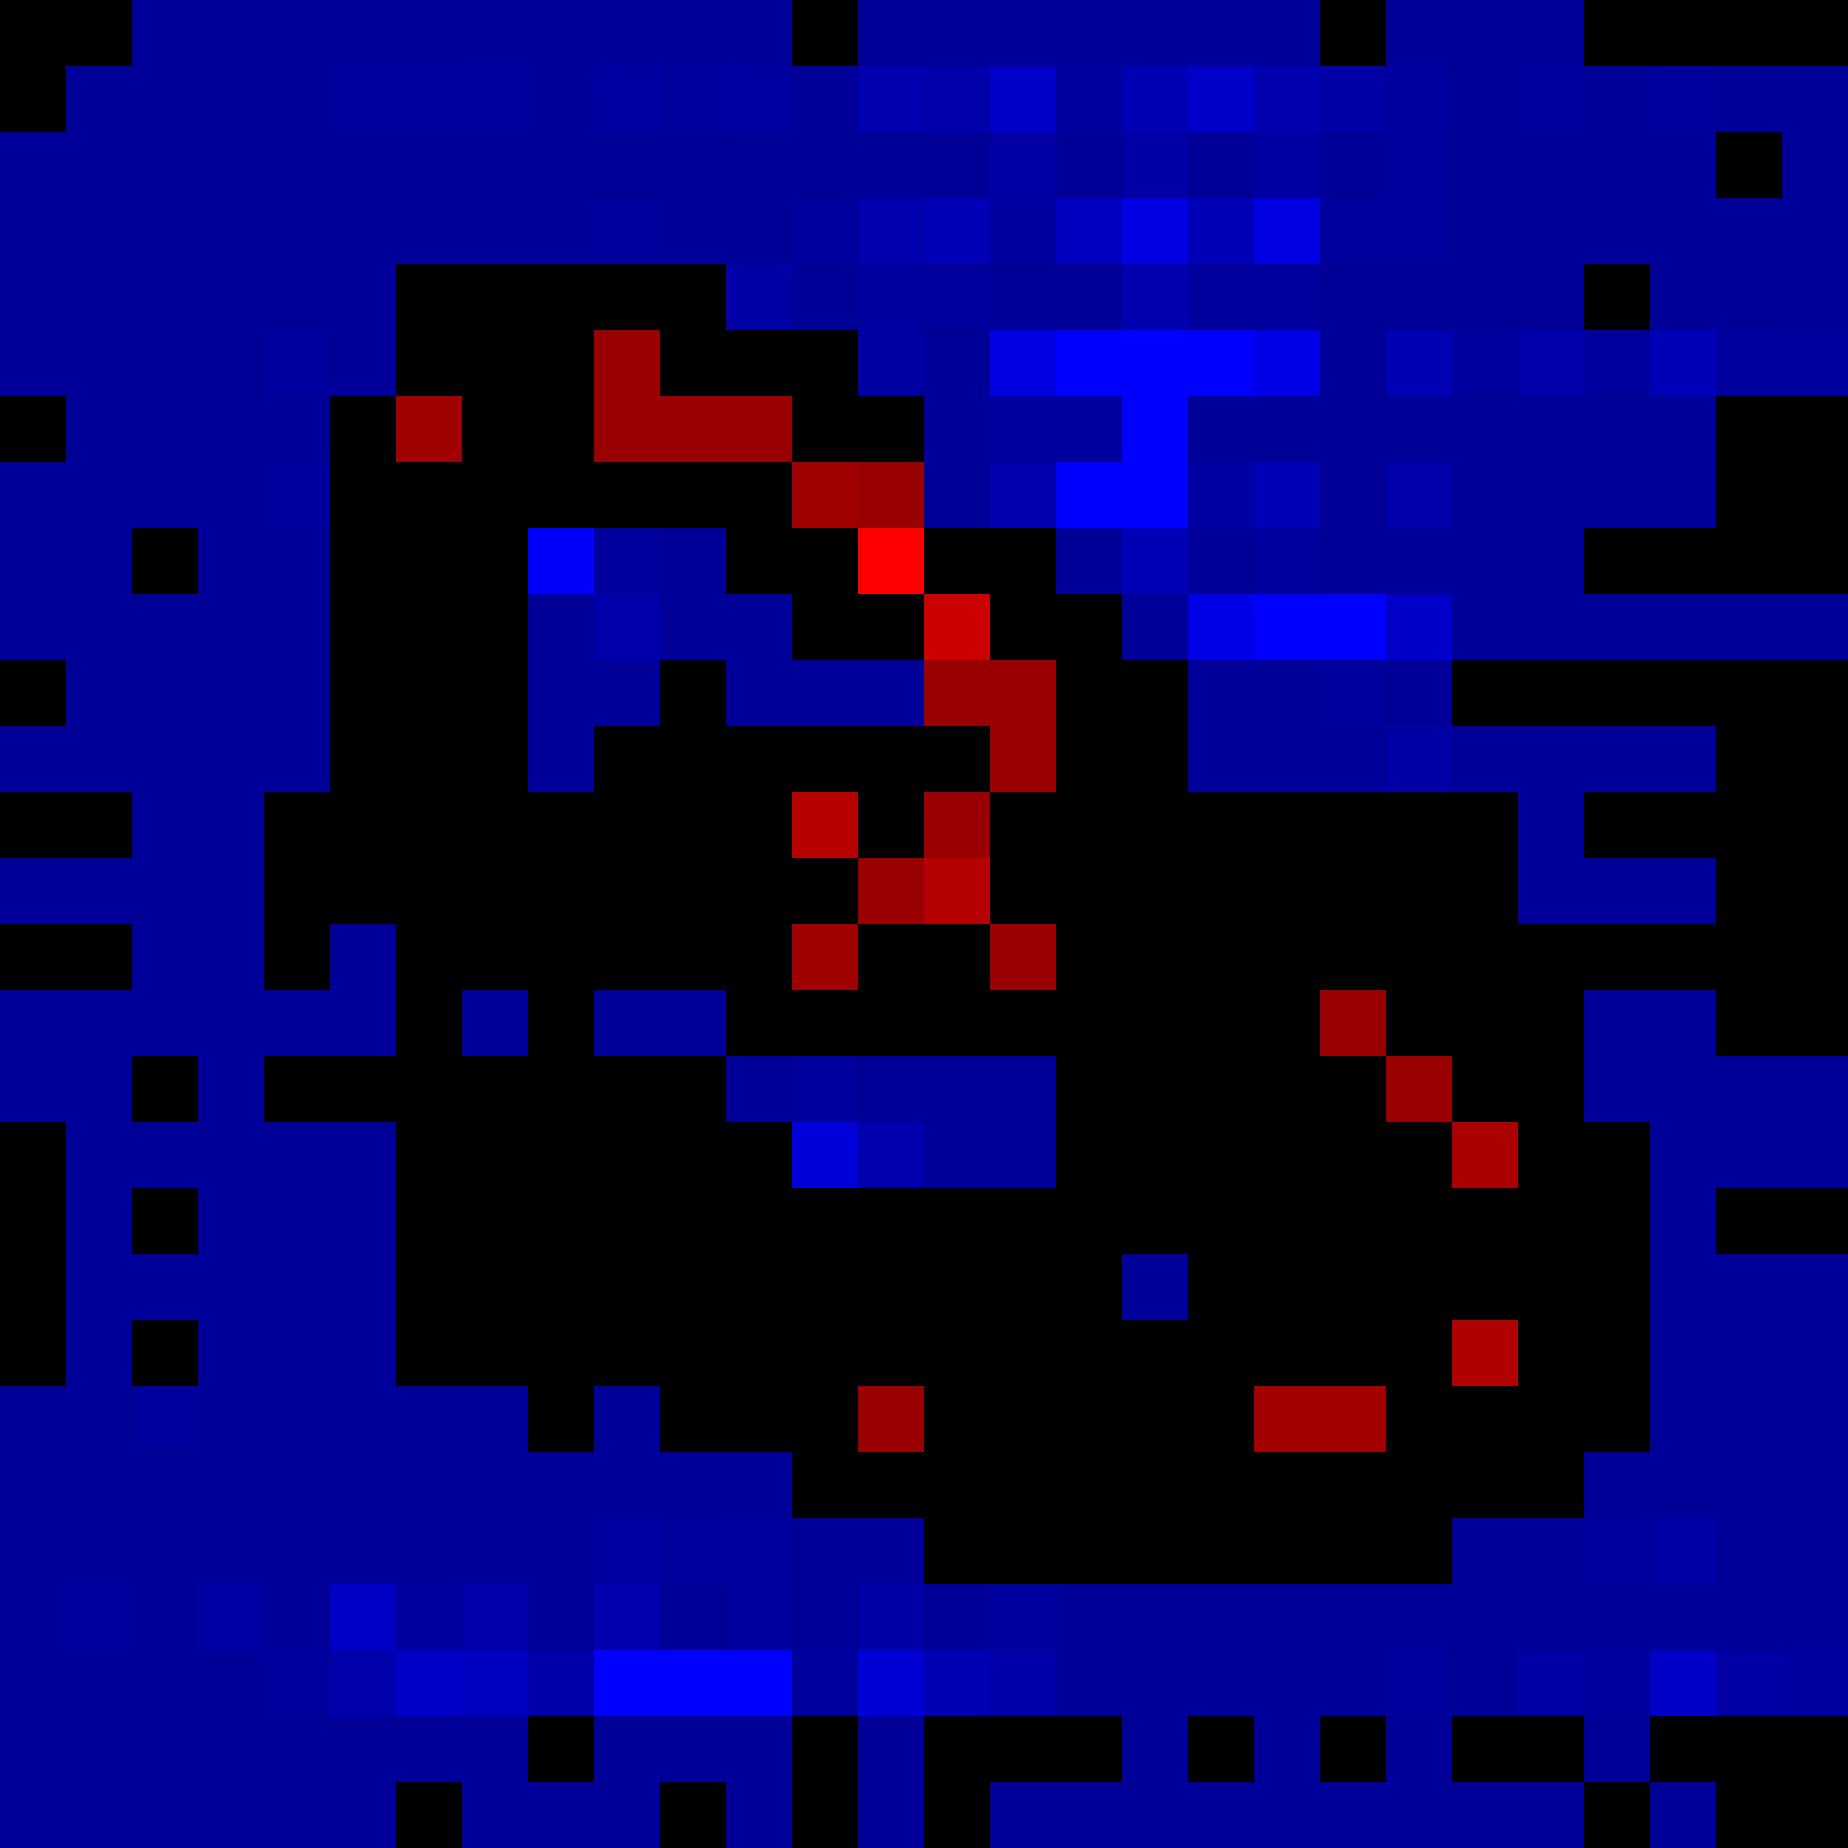
\includegraphics[width=\linewidth]{saliency/mnist_split_ic_saliency/image_030_true_3_pred_3/final_saliency_threshold_wrt_3_bright.png}\\[-1pt]{\scriptsize Logit 3}
		\end{minipage}%
		\begin{minipage}[b]{0.19\linewidth}\centering
			
\includegraphics[width=\linewidth]{saliency/mnist_split_ic_saliency/image_030_true_3_pred_3/final_saliency_threshold_wrt_4_bright.png}\\[-1pt]{\scriptsize Logit 4}
		\end{minipage}

		\vspace{0.12cm}

		\begin{minipage}[b]{0.19\linewidth}\centering
			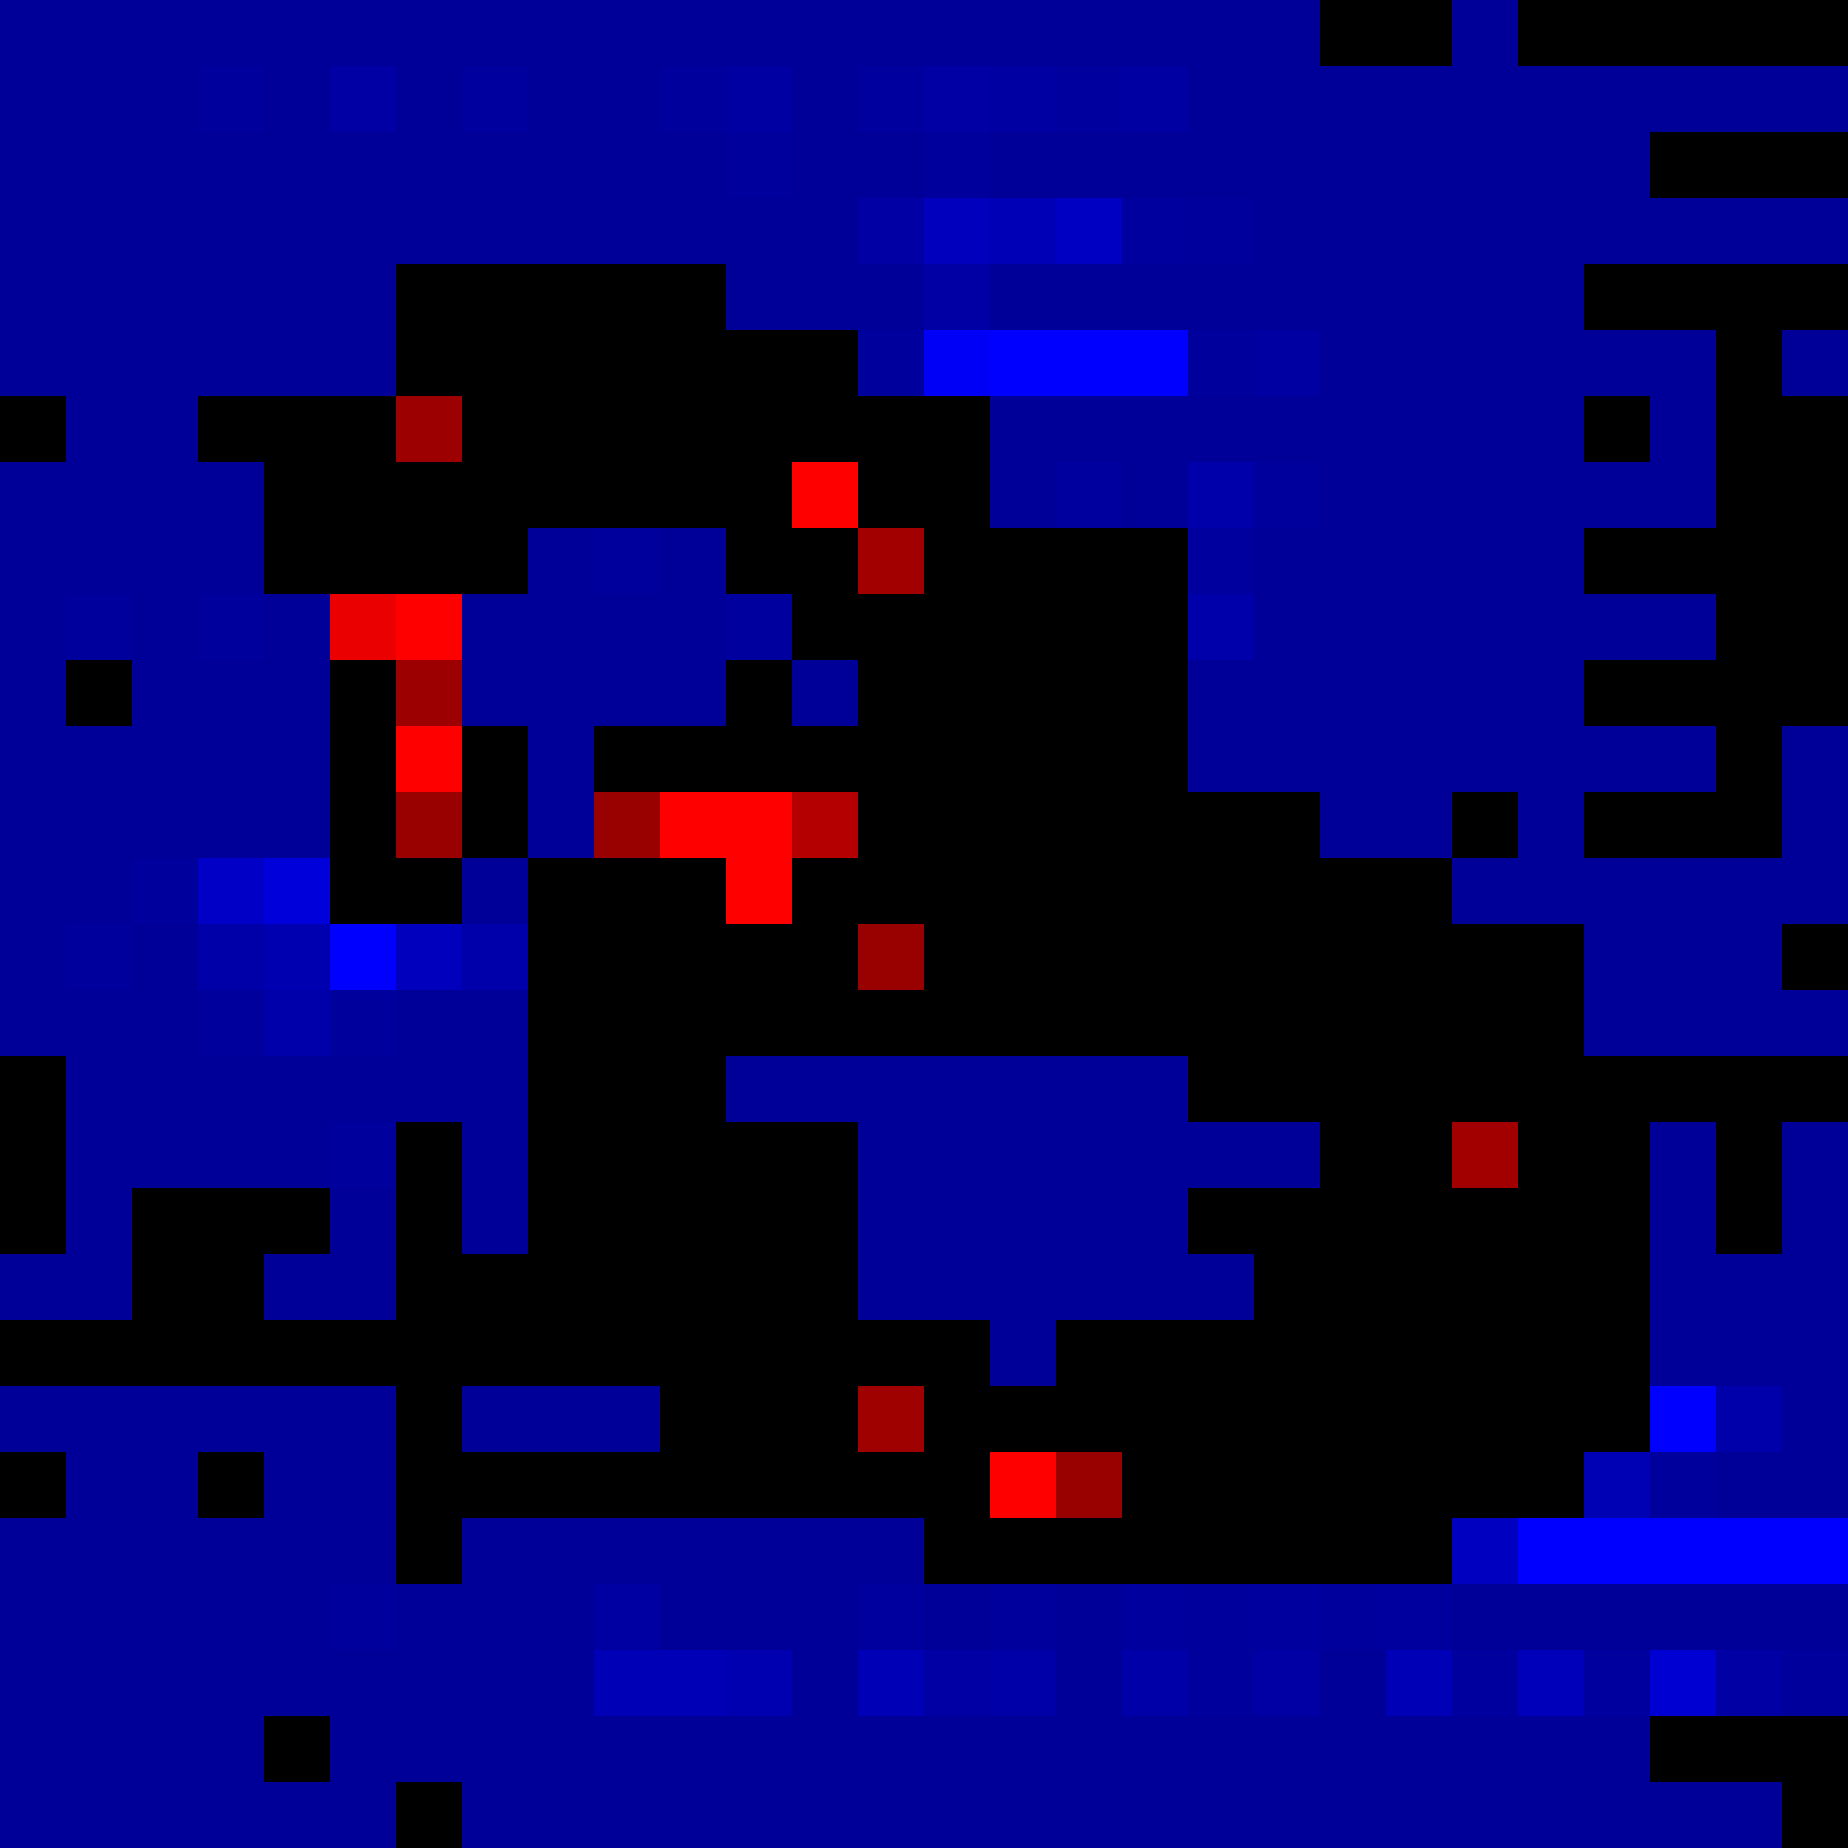
\includegraphics[width=\linewidth]{saliency/mnist_split_ic_saliency/image_030_true_3_pred_3/final_saliency_threshold_wrt_5_bright.png}\\[-1pt]{\scriptsize Logit 5}
		\end{minipage}%
		\begin{minipage}[b]{0.19\linewidth}\centering
			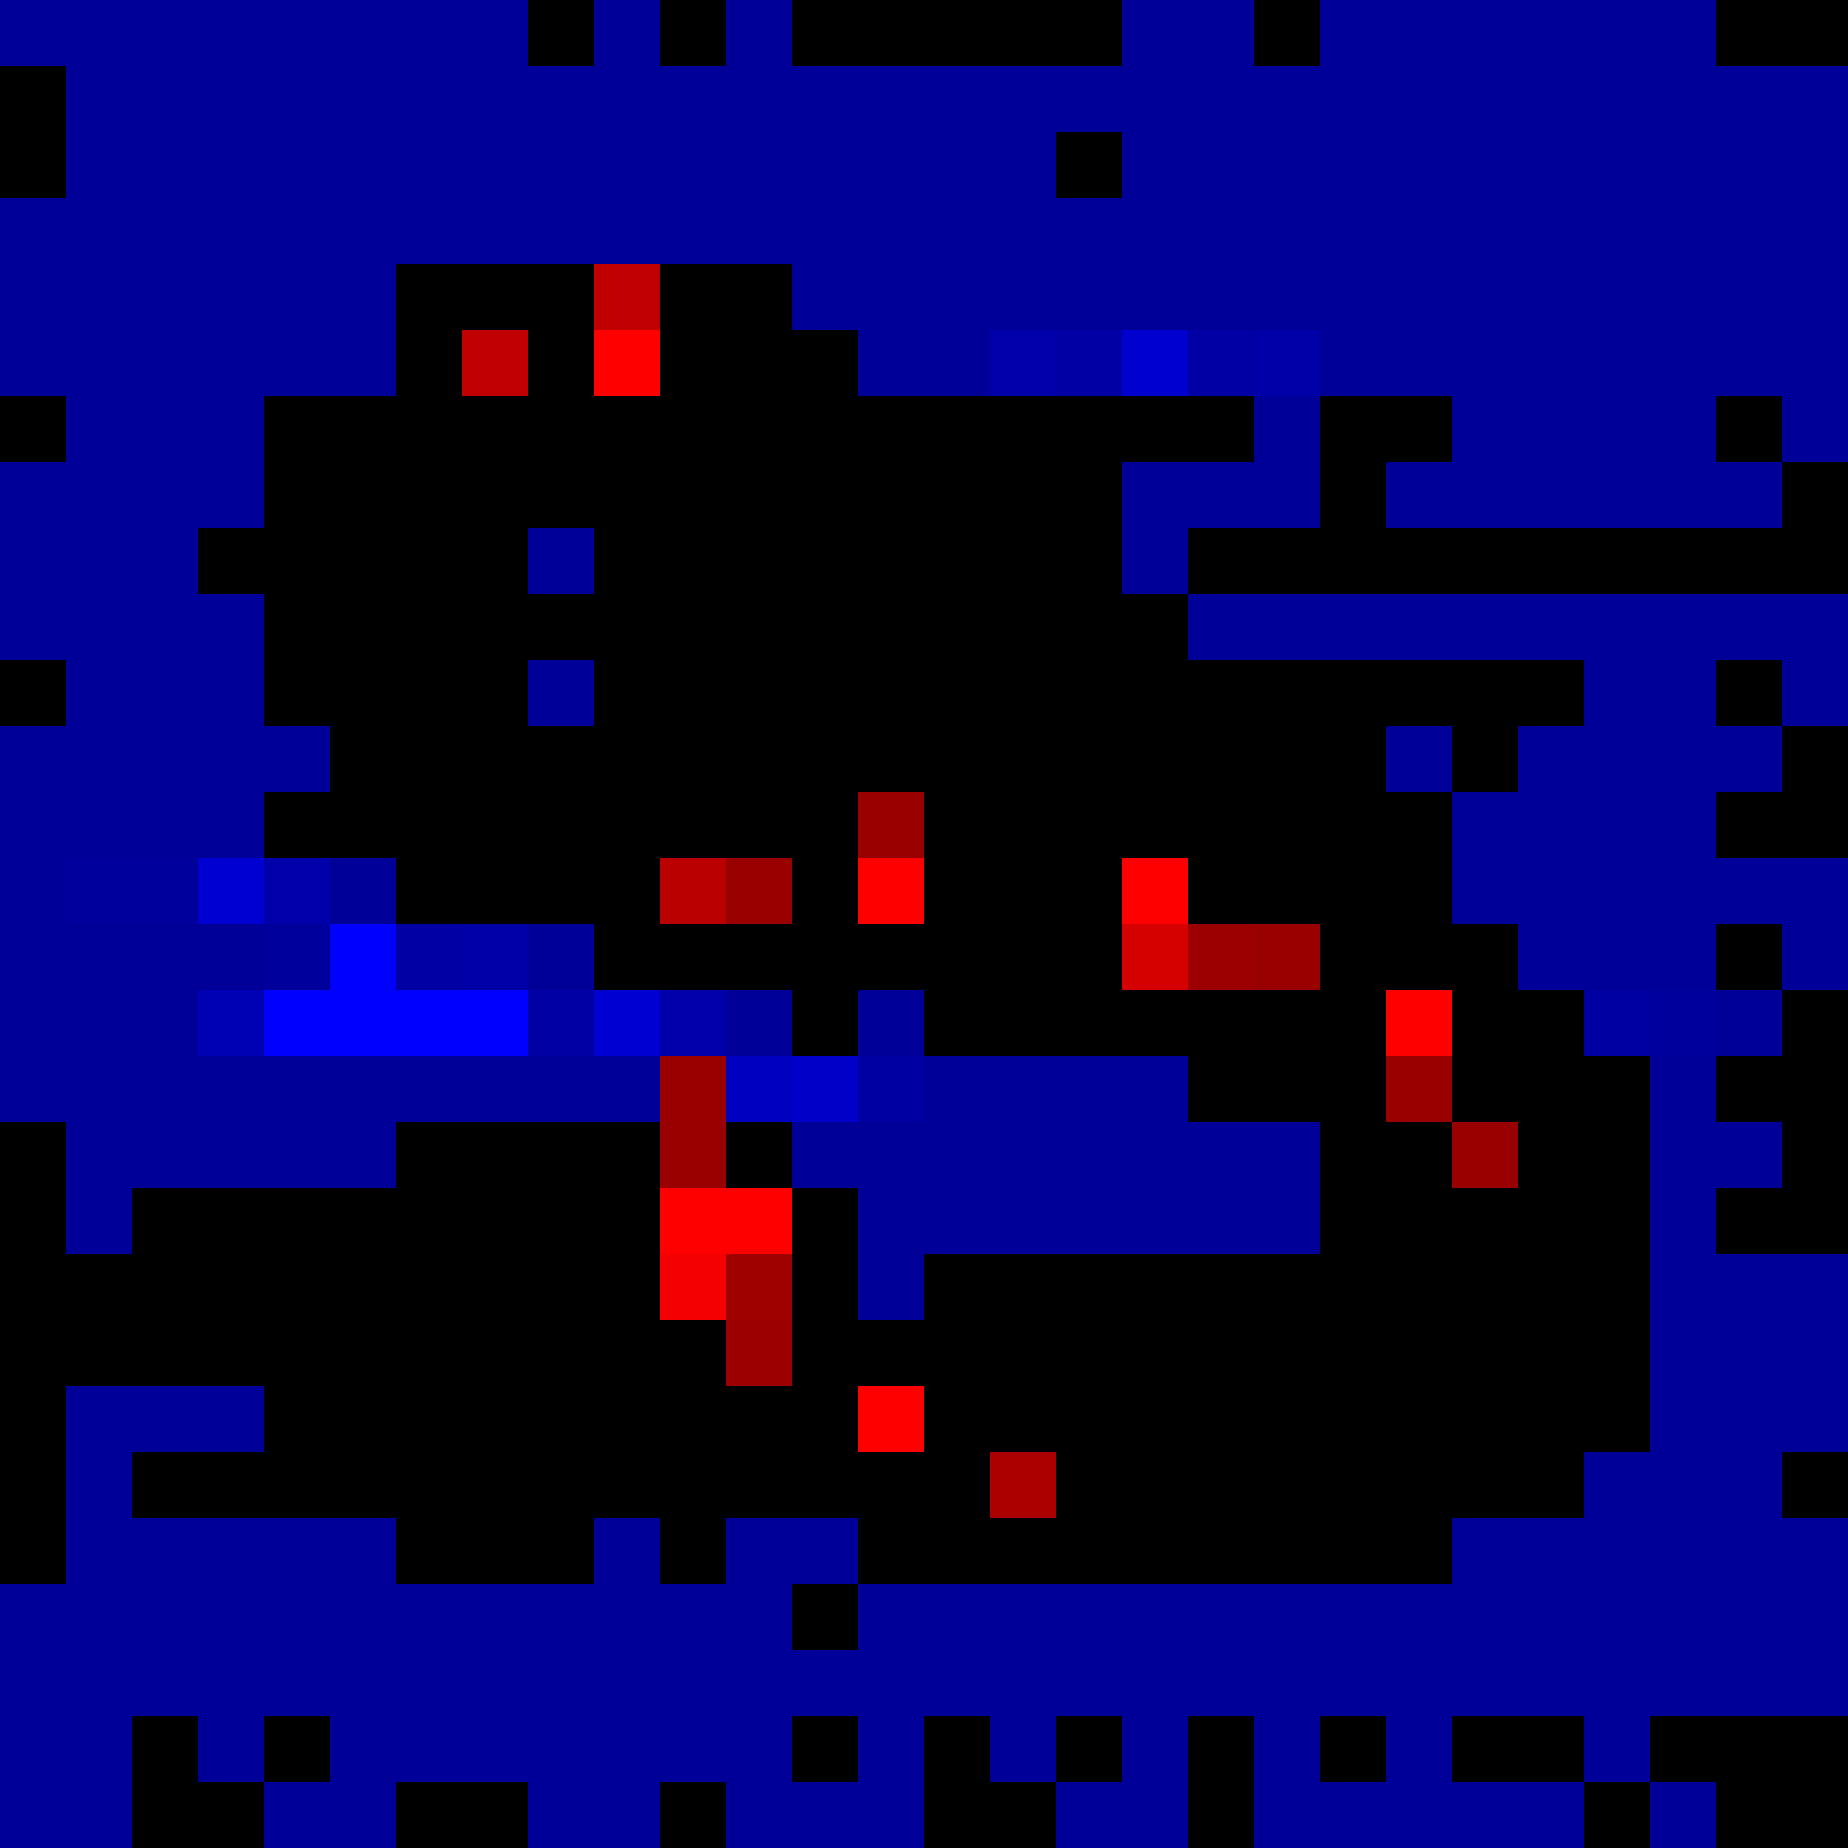
\includegraphics[width=\linewidth]{saliency/mnist_split_ic_saliency/image_030_true_3_pred_3/final_saliency_threshold_wrt_6_bright.png}\\[-1pt]{\scriptsize Logit 6}
		\end{minipage}%
		\begin{minipage}[b]{0.19\linewidth}\centering
			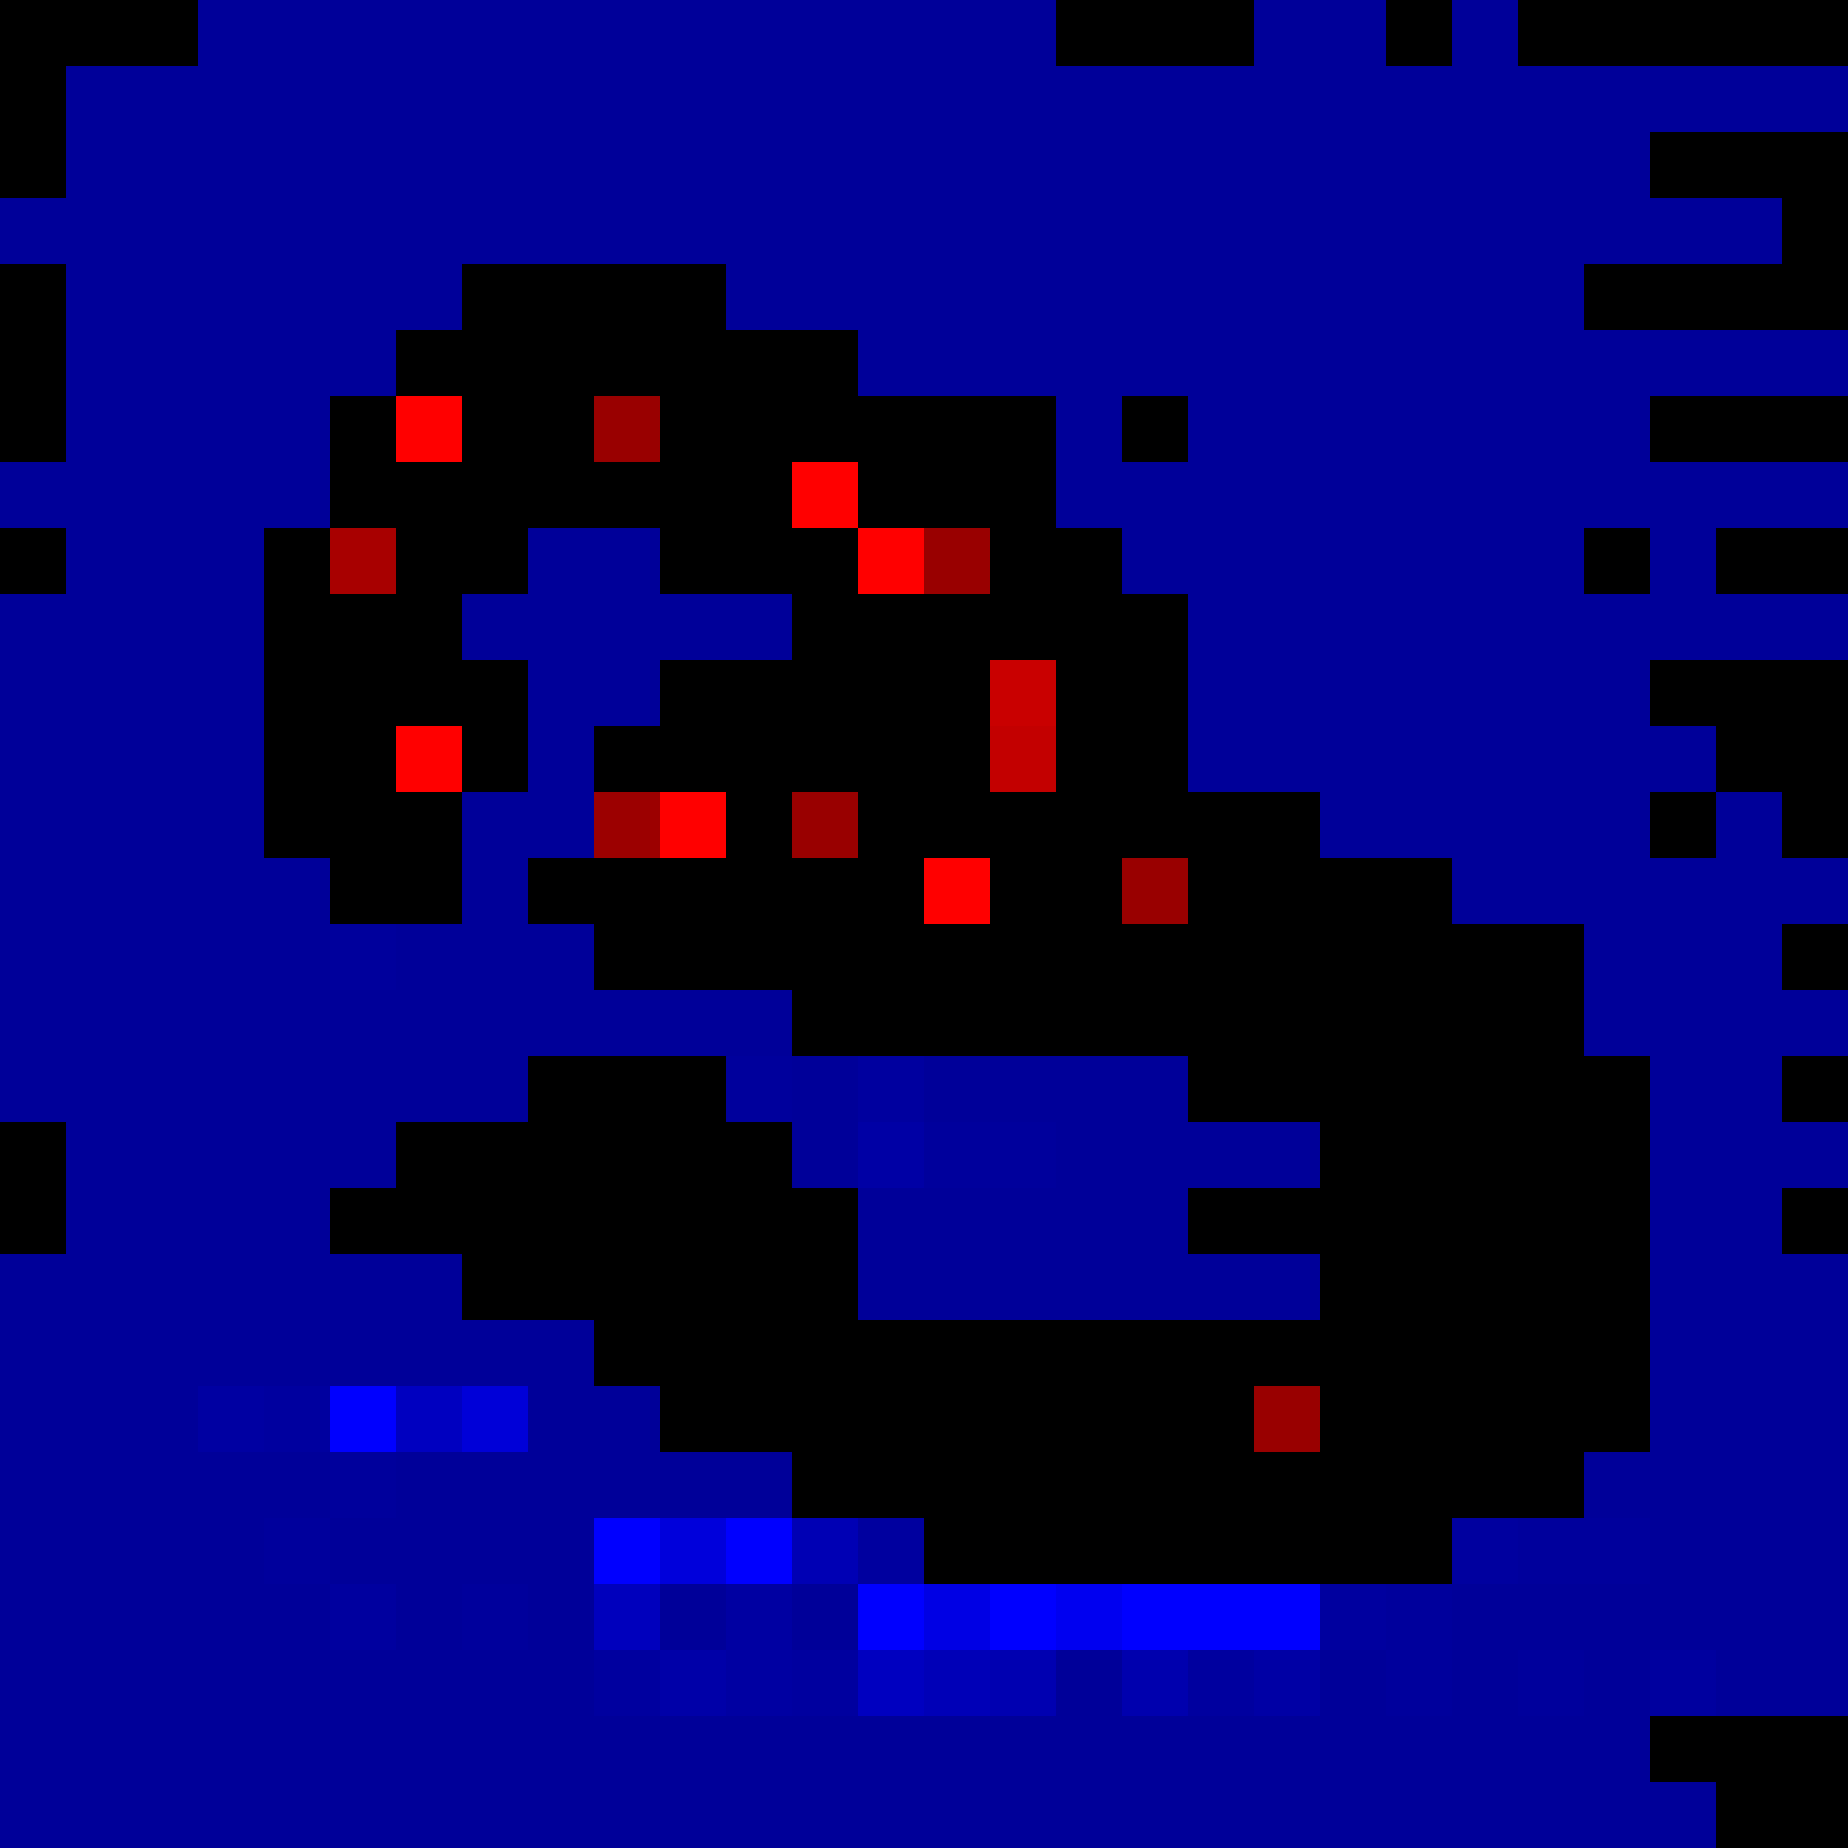
\includegraphics[width=\linewidth]{saliency/mnist_split_ic_saliency/image_030_true_3_pred_3/final_saliency_threshold_wrt_7_bright.png}\\[-1pt]{\scriptsize Logit 7}
		\end{minipage}%
		\begin{minipage}[b]{0.19\linewidth}\centering
			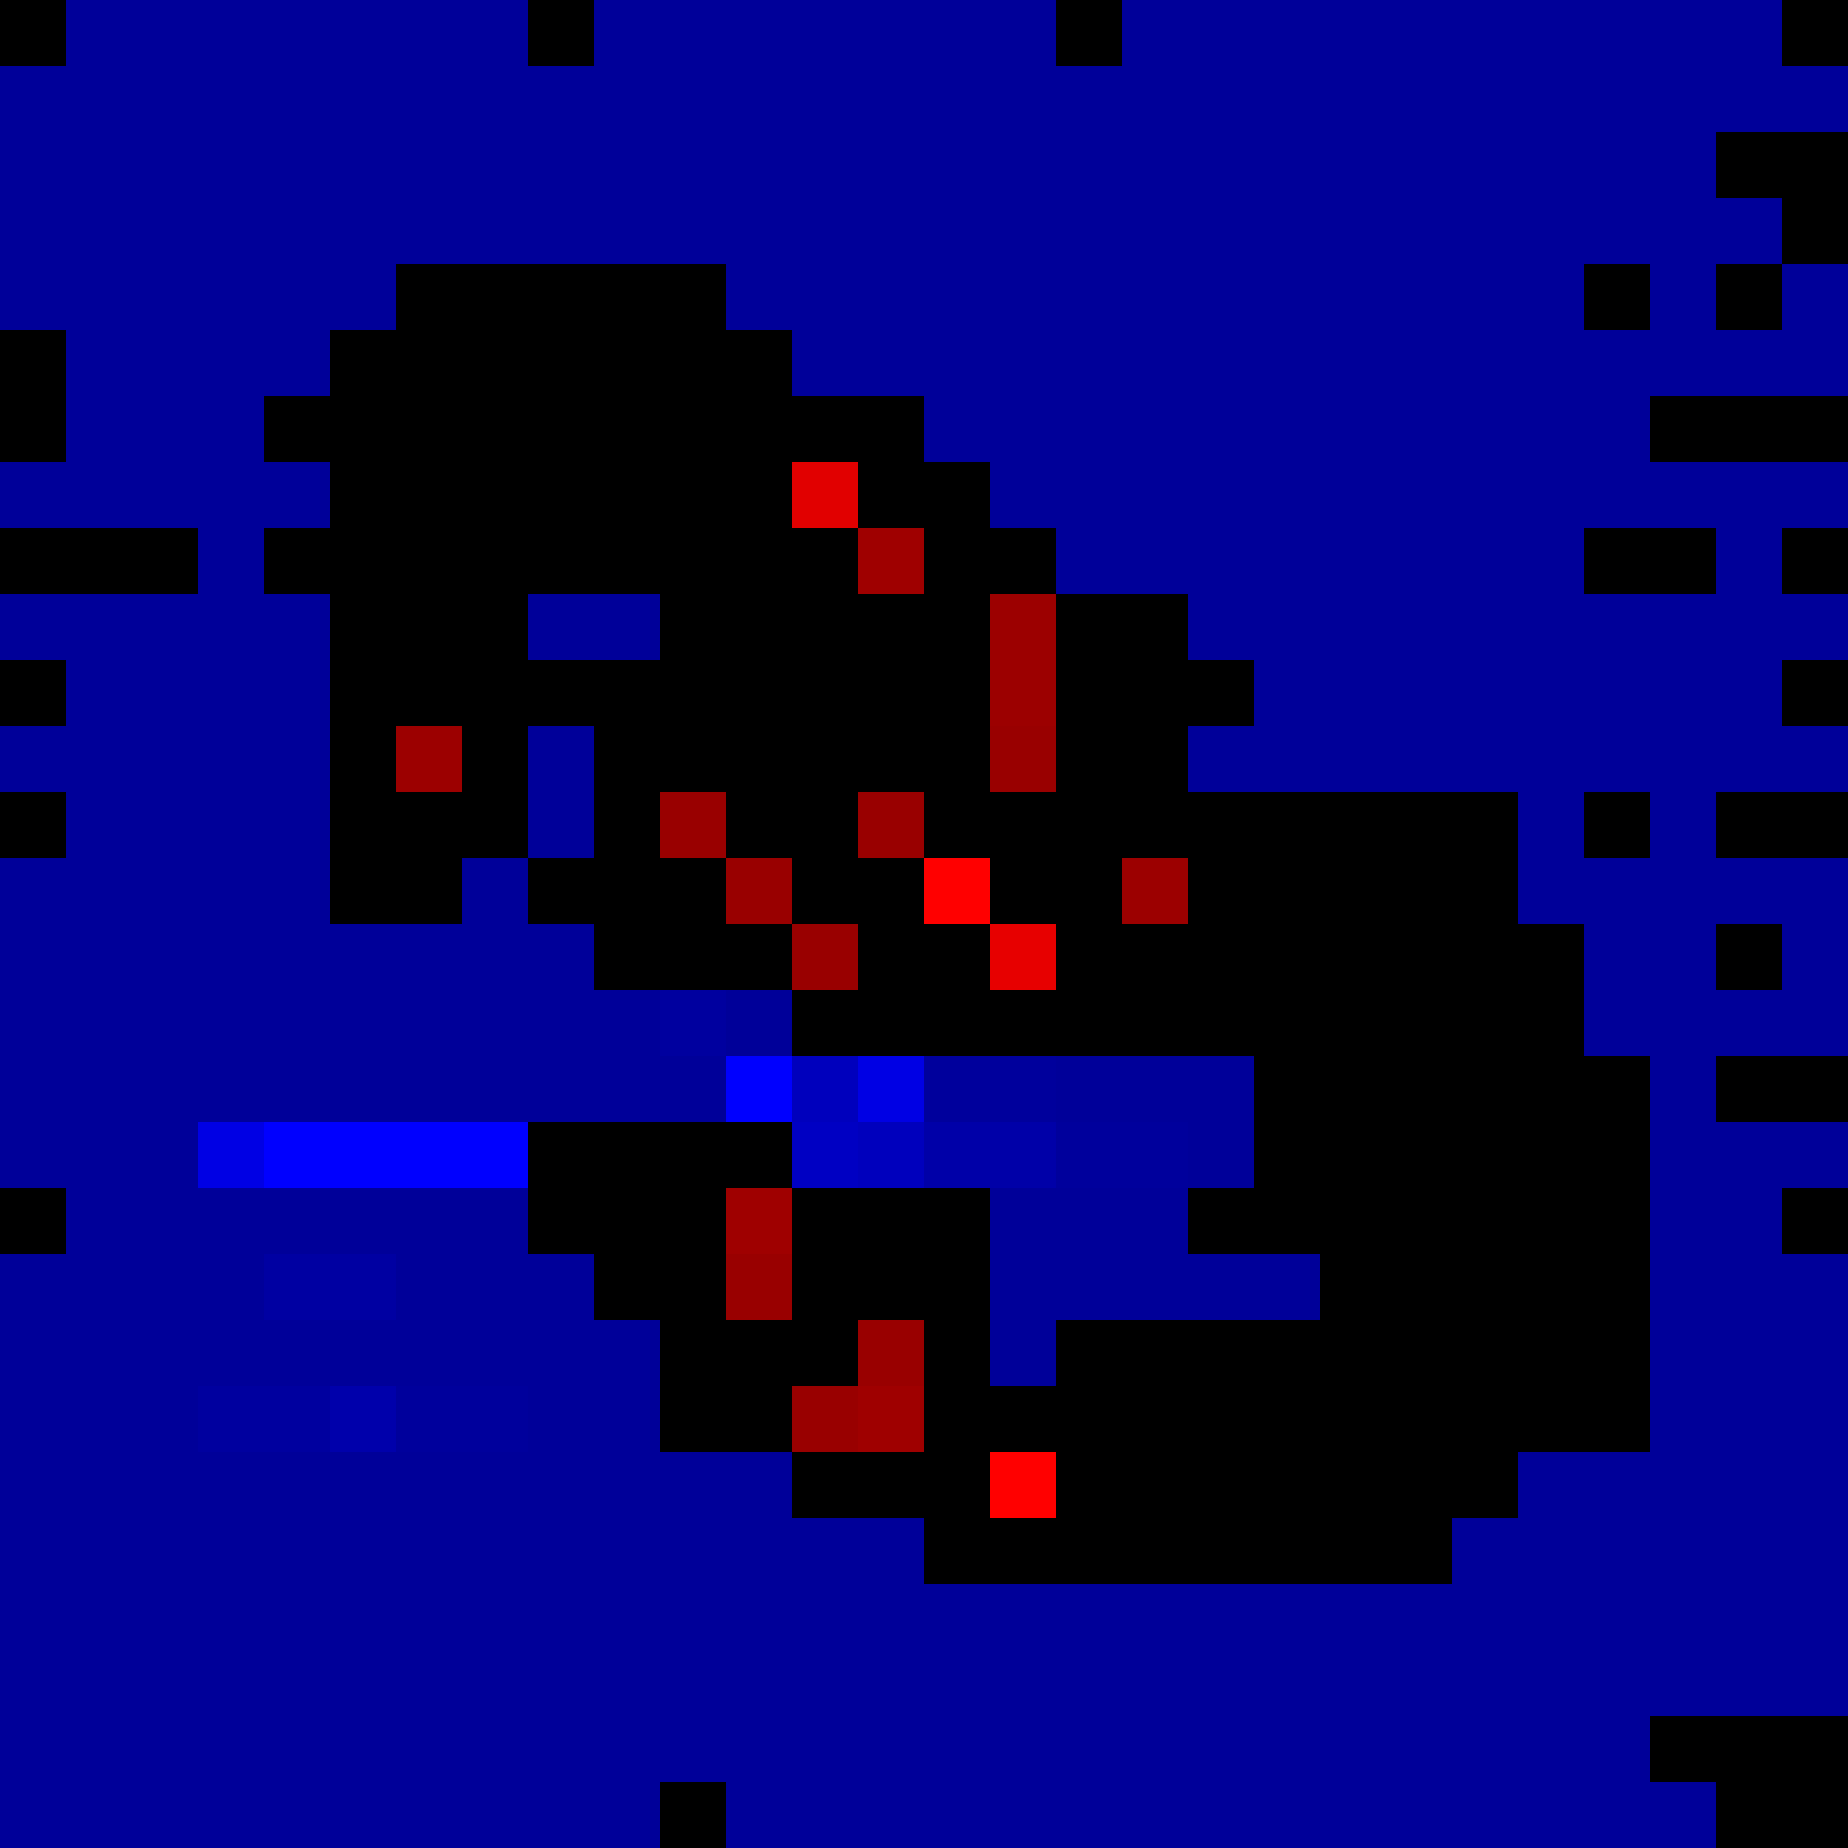
\includegraphics[width=\linewidth]{saliency/mnist_split_ic_saliency/image_030_true_3_pred_3/final_saliency_threshold_wrt_8_bright.png}\\[-1pt]{\scriptsize Logit 8}
		\end{minipage}%
		\begin{minipage}[b]{0.19\linewidth}\centering
			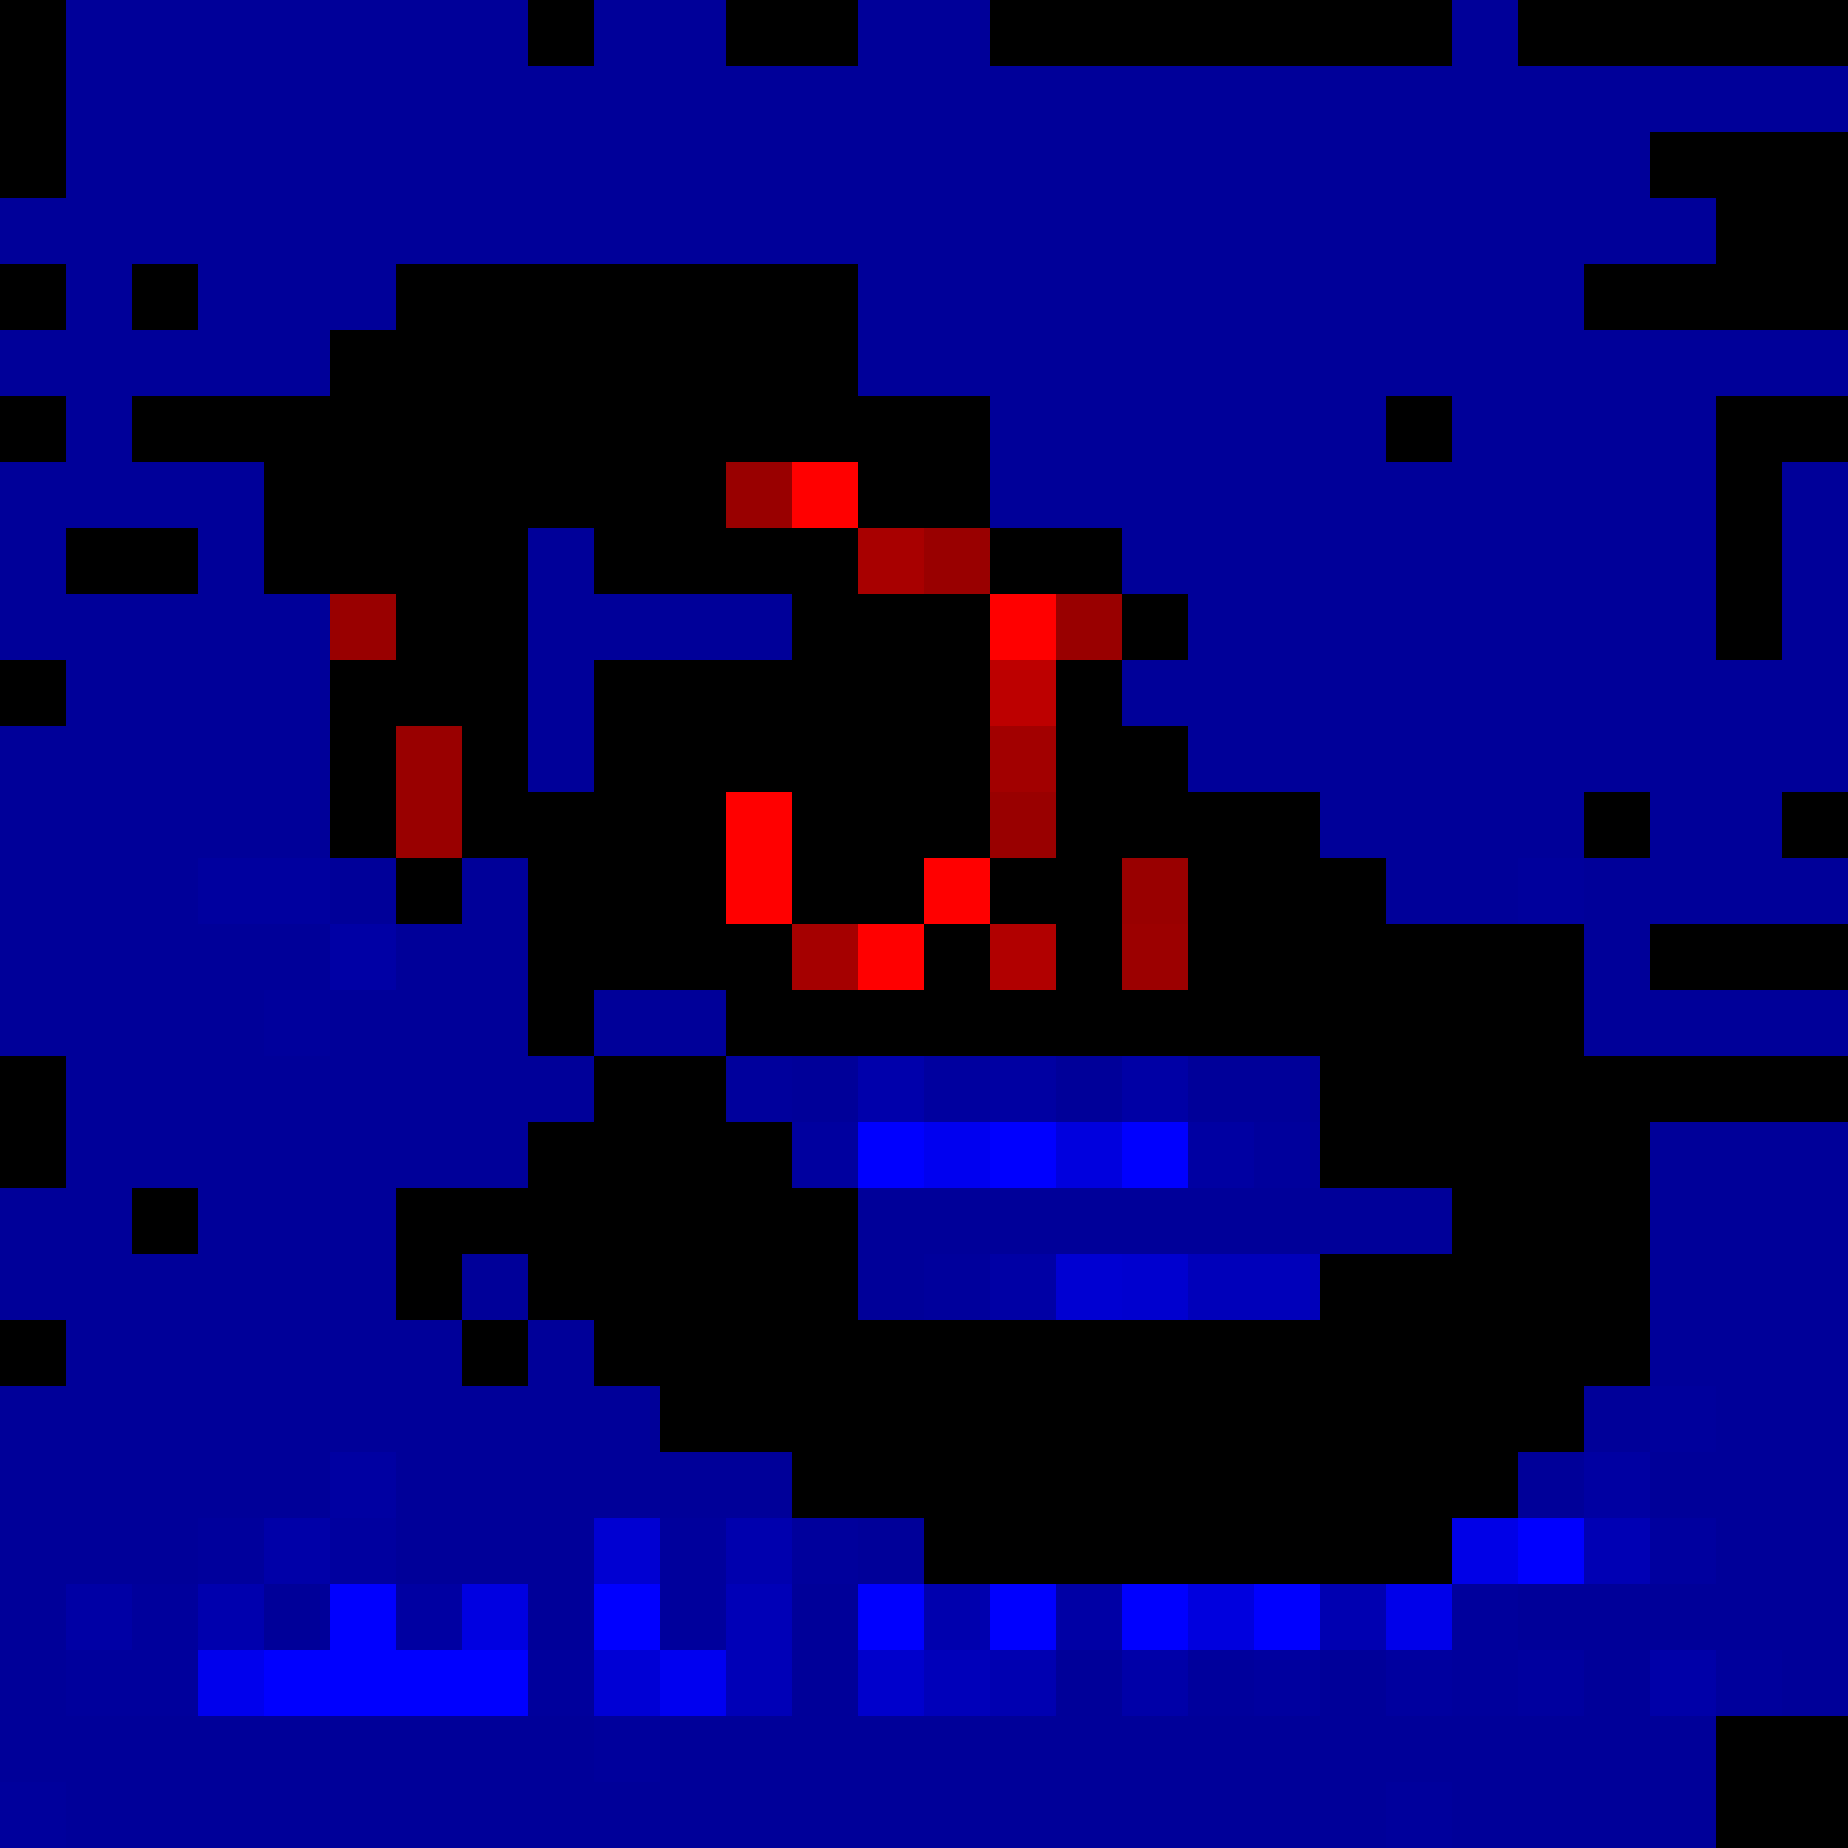
\includegraphics[width=\linewidth]{saliency/mnist_split_ic_saliency/image_030_true_3_pred_3/final_saliency_threshold_wrt_9_bright.png}\\[-1pt]{\scriptsize Logit 9}
		\end{minipage}
	\end{minipage}
	}%
\caption[Stream gradients of the inverted-input DIC model]{Stream gradients of the inverted-input DIC model (\texttt{cnn\_maxout} DICIN) on a correctly classified MNIST test digit ``3'', thresholded and overlaid per class logit. The $g$-stream gradient (red) highlights sensitivities on present strokes, while the $h$-stream gradient (blue) highlights sensitivities at candidate missing-stroke locations. These stream-local maps do not by themselves establish the effect of adding pixels on the complete model. Left: the original digit.}
	\label{fig:mnist_split_ic_saliency}
\end{figure}

\begin{figure}[t]
\QualitativeImageContent{
	\centering
	\begin{minipage}[c]{0.15\linewidth}
		\centering
		
\includegraphics[width=\linewidth]{saliency/mnist_split_ic_saliency/image_036_true_3_pred_3/original.png}\\[-1pt]
		{\scriptsize Original}
	\end{minipage}\hspace{0.015\linewidth}%
	\begin{minipage}[c]{0.80\linewidth}
		\centering
		\begin{minipage}[b]{0.19\linewidth}\centering
			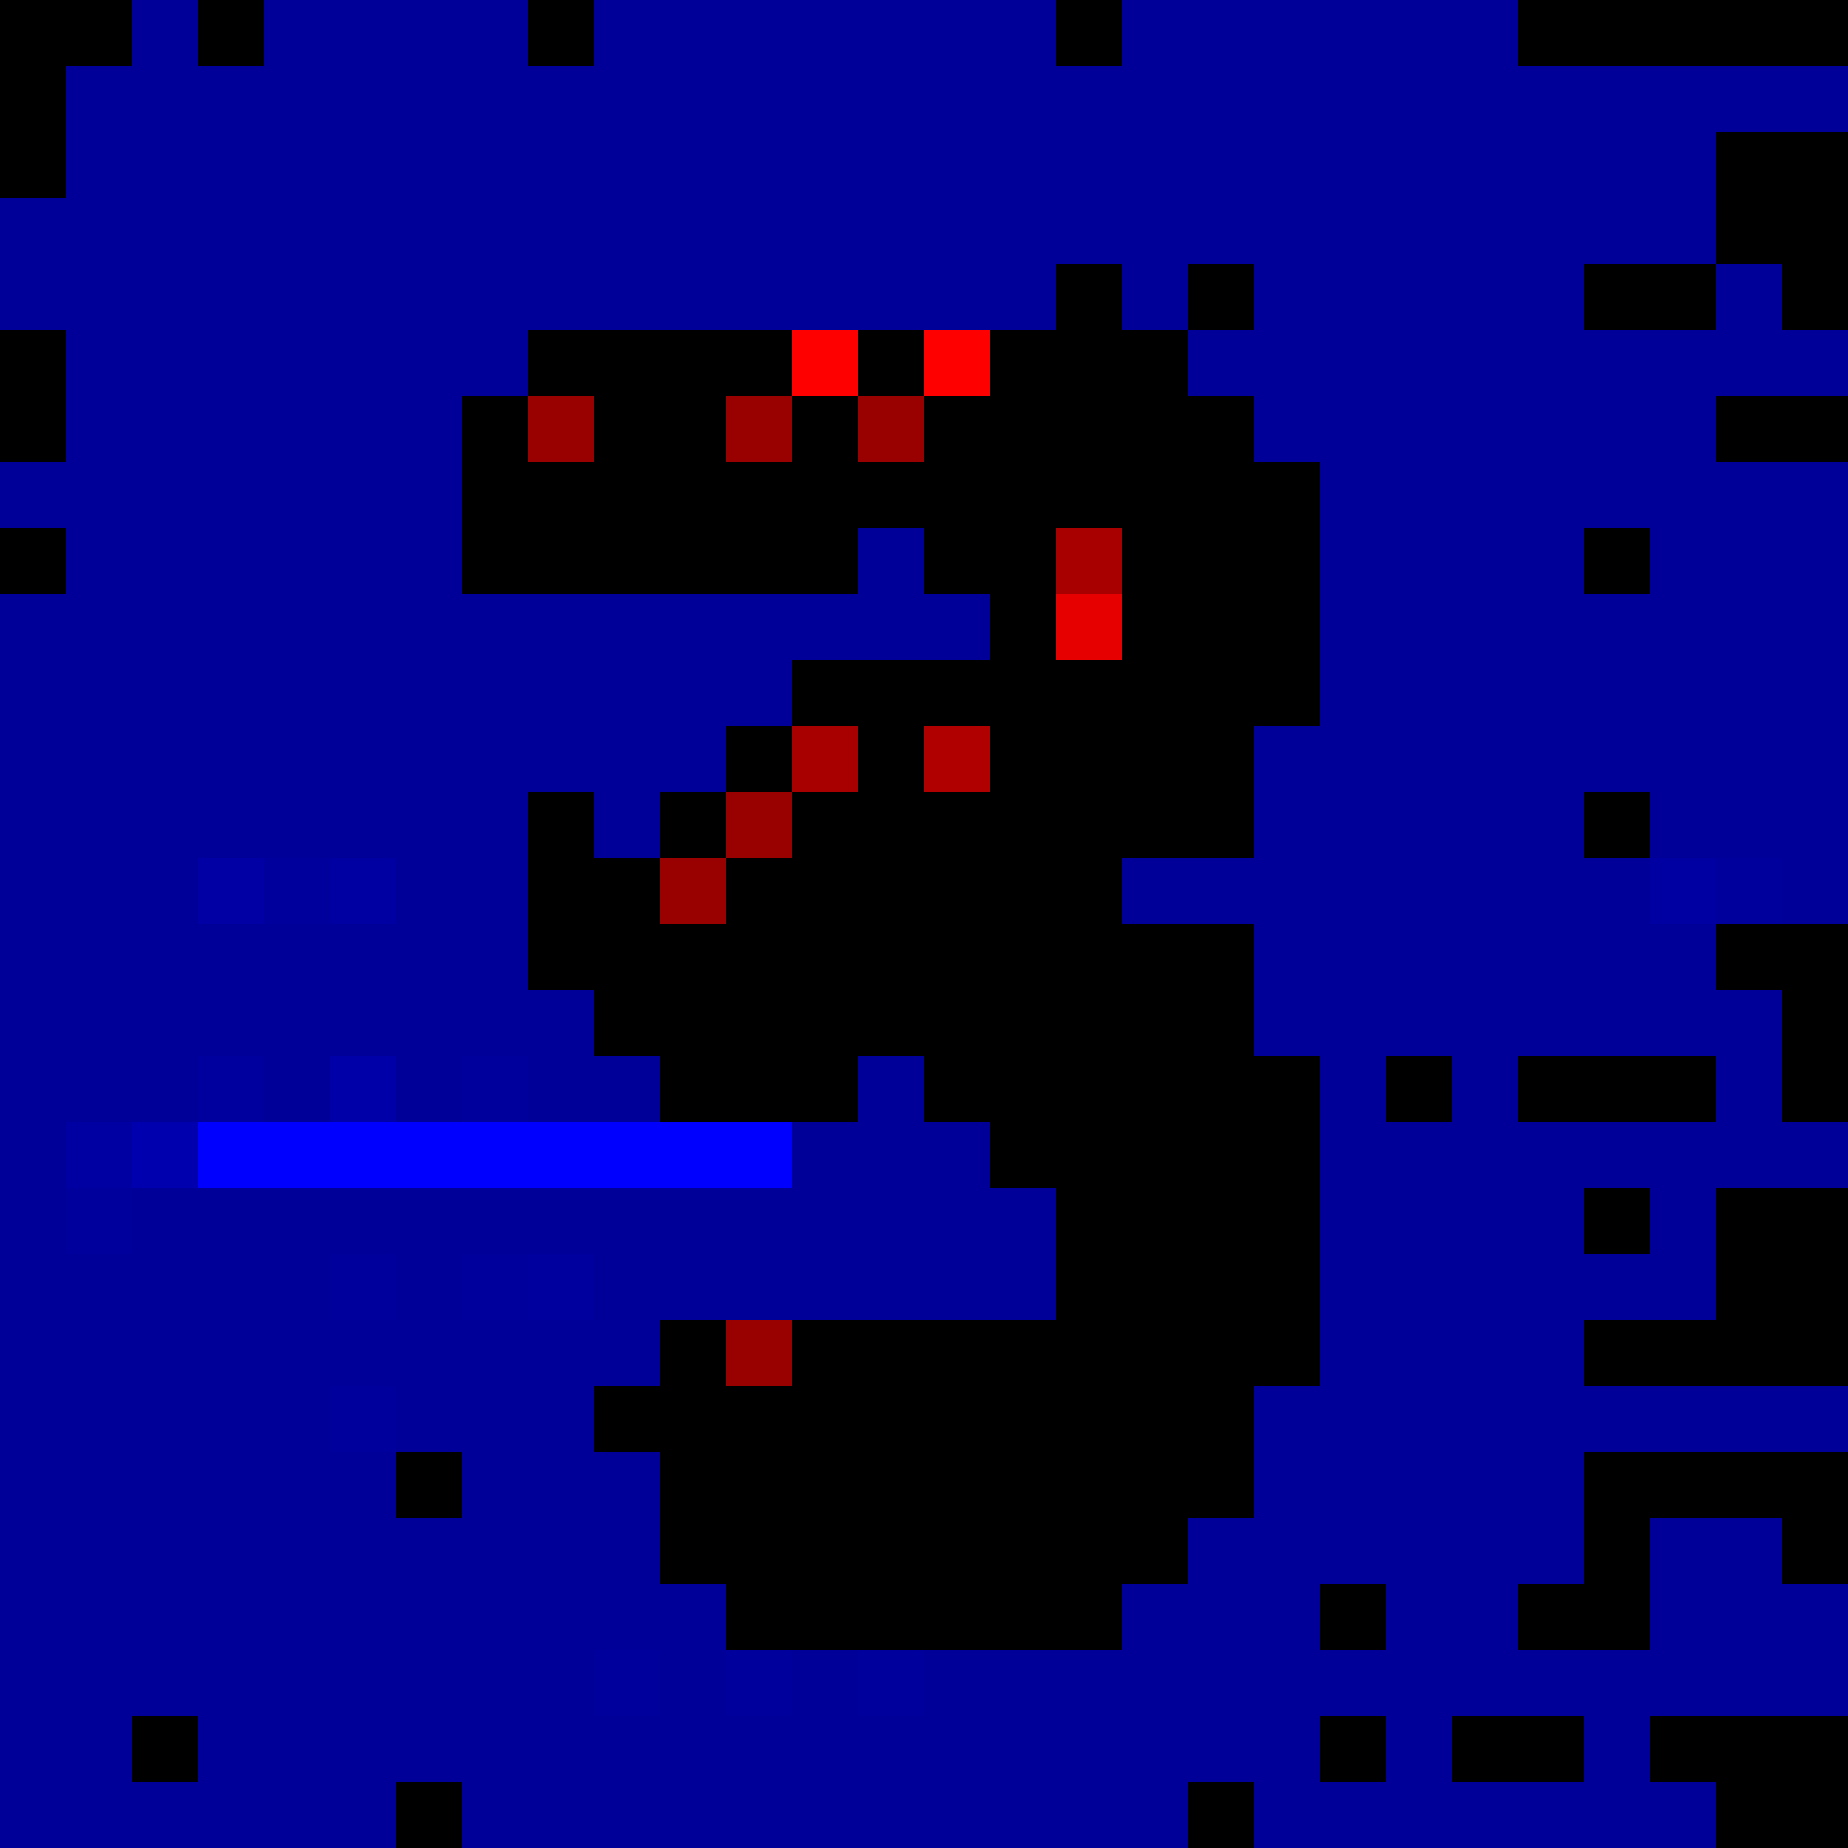
\includegraphics[width=\linewidth]{saliency/mnist_split_ic_saliency/image_036_true_3_pred_3/final_saliency_threshold_wrt_0_bright.png}\\[-1pt]{\scriptsize Logit 0}
		\end{minipage}%
		\begin{minipage}[b]{0.19\linewidth}\centering
			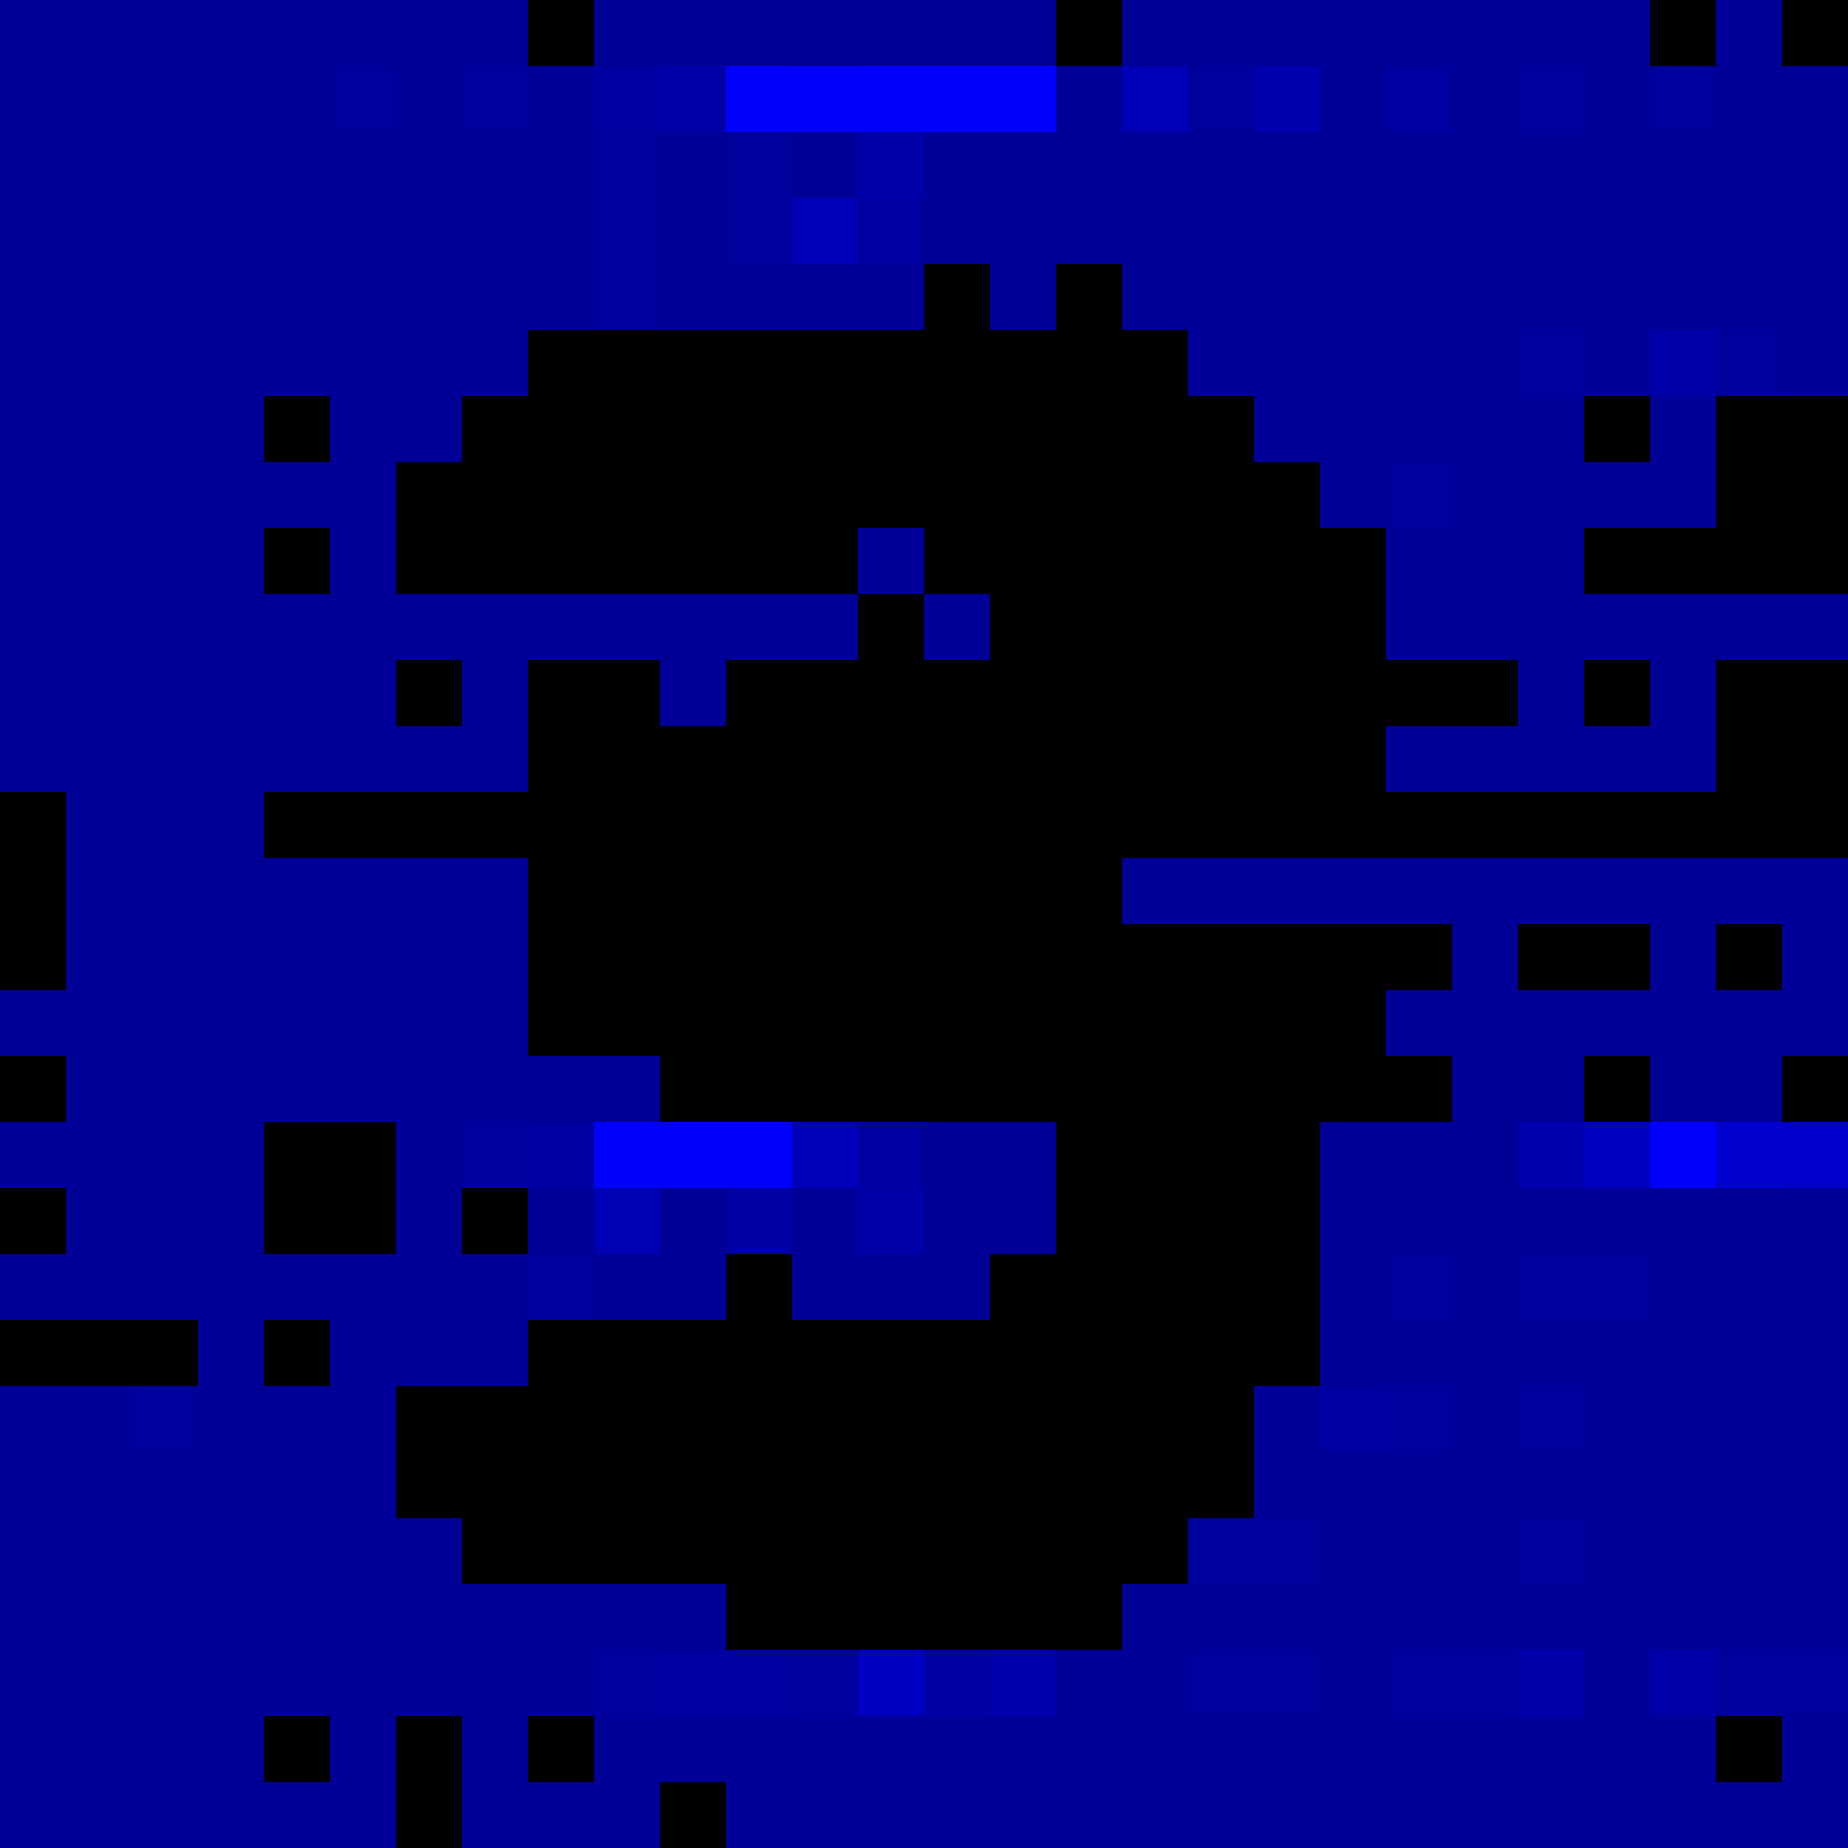
\includegraphics[width=\linewidth]{saliency/mnist_split_ic_saliency/image_036_true_3_pred_3/final_saliency_threshold_wrt_1_bright.png}\\[-1pt]{\scriptsize Logit 1}
		\end{minipage}%
		\begin{minipage}[b]{0.19\linewidth}\centering
			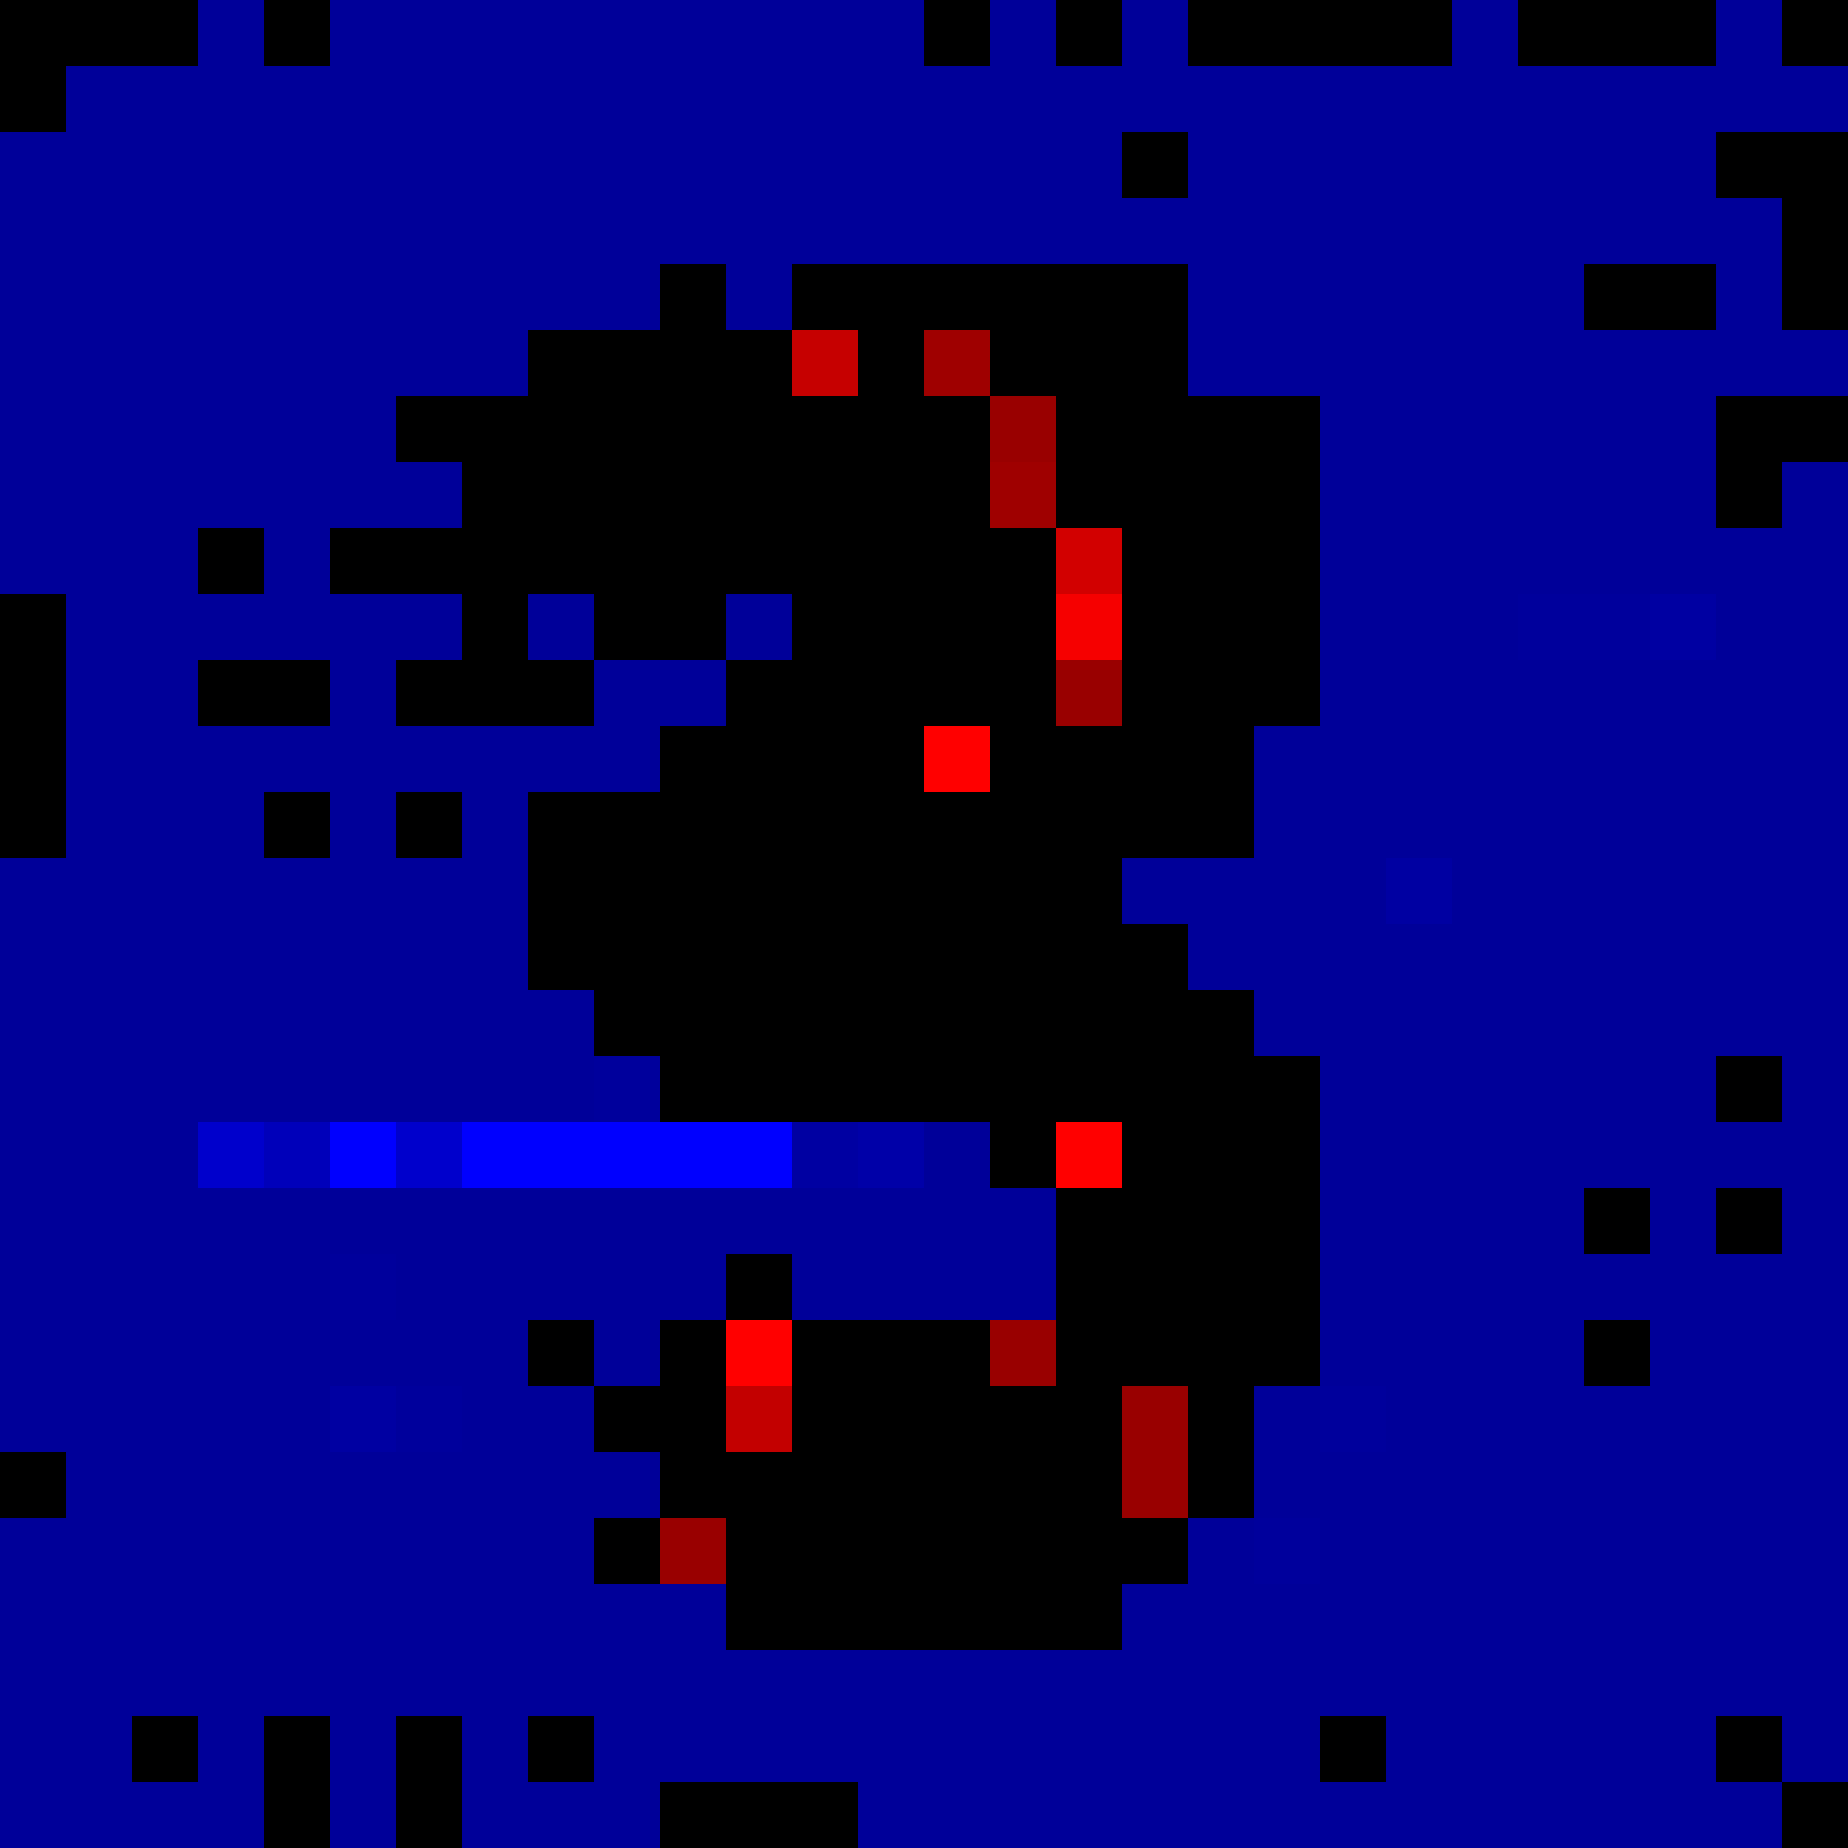
\includegraphics[width=\linewidth]{saliency/mnist_split_ic_saliency/image_036_true_3_pred_3/final_saliency_threshold_wrt_2_bright.png}\\[-1pt]{\scriptsize Logit 2}
		\end{minipage}%
		\begin{minipage}[b]{0.19\linewidth}\centering
			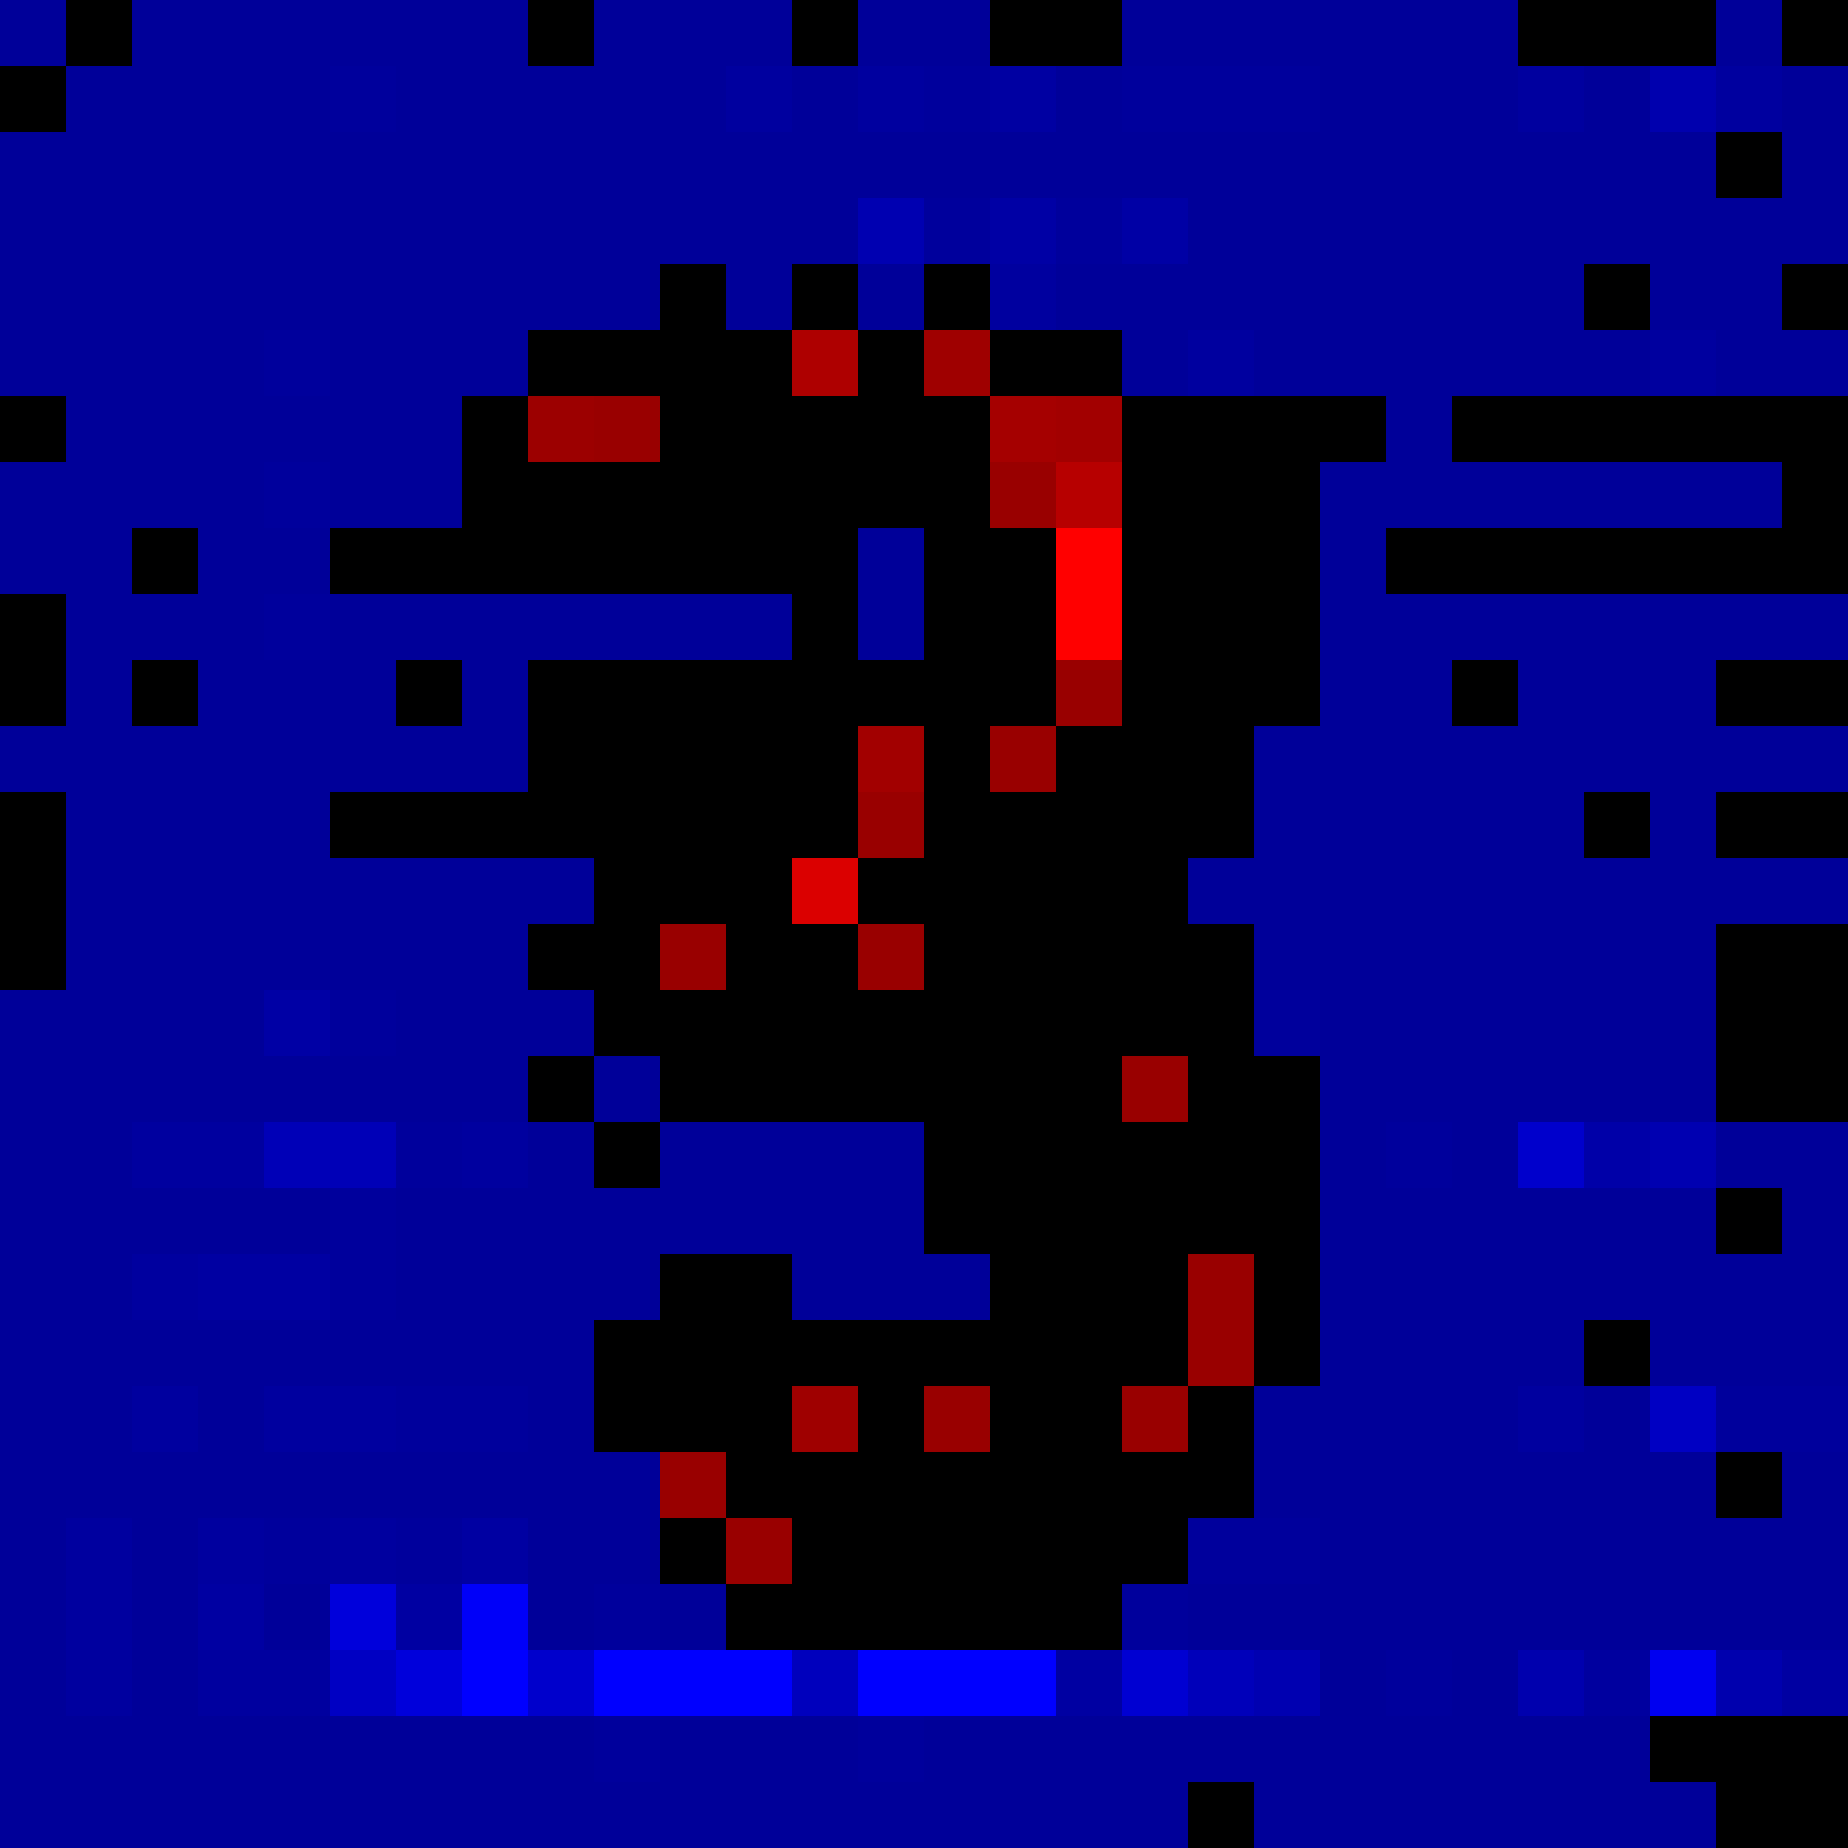
\includegraphics[width=\linewidth]{saliency/mnist_split_ic_saliency/image_036_true_3_pred_3/final_saliency_threshold_wrt_3_bright.png}\\[-1pt]{\scriptsize Logit 3}
		\end{minipage}%
		\begin{minipage}[b]{0.19\linewidth}\centering
			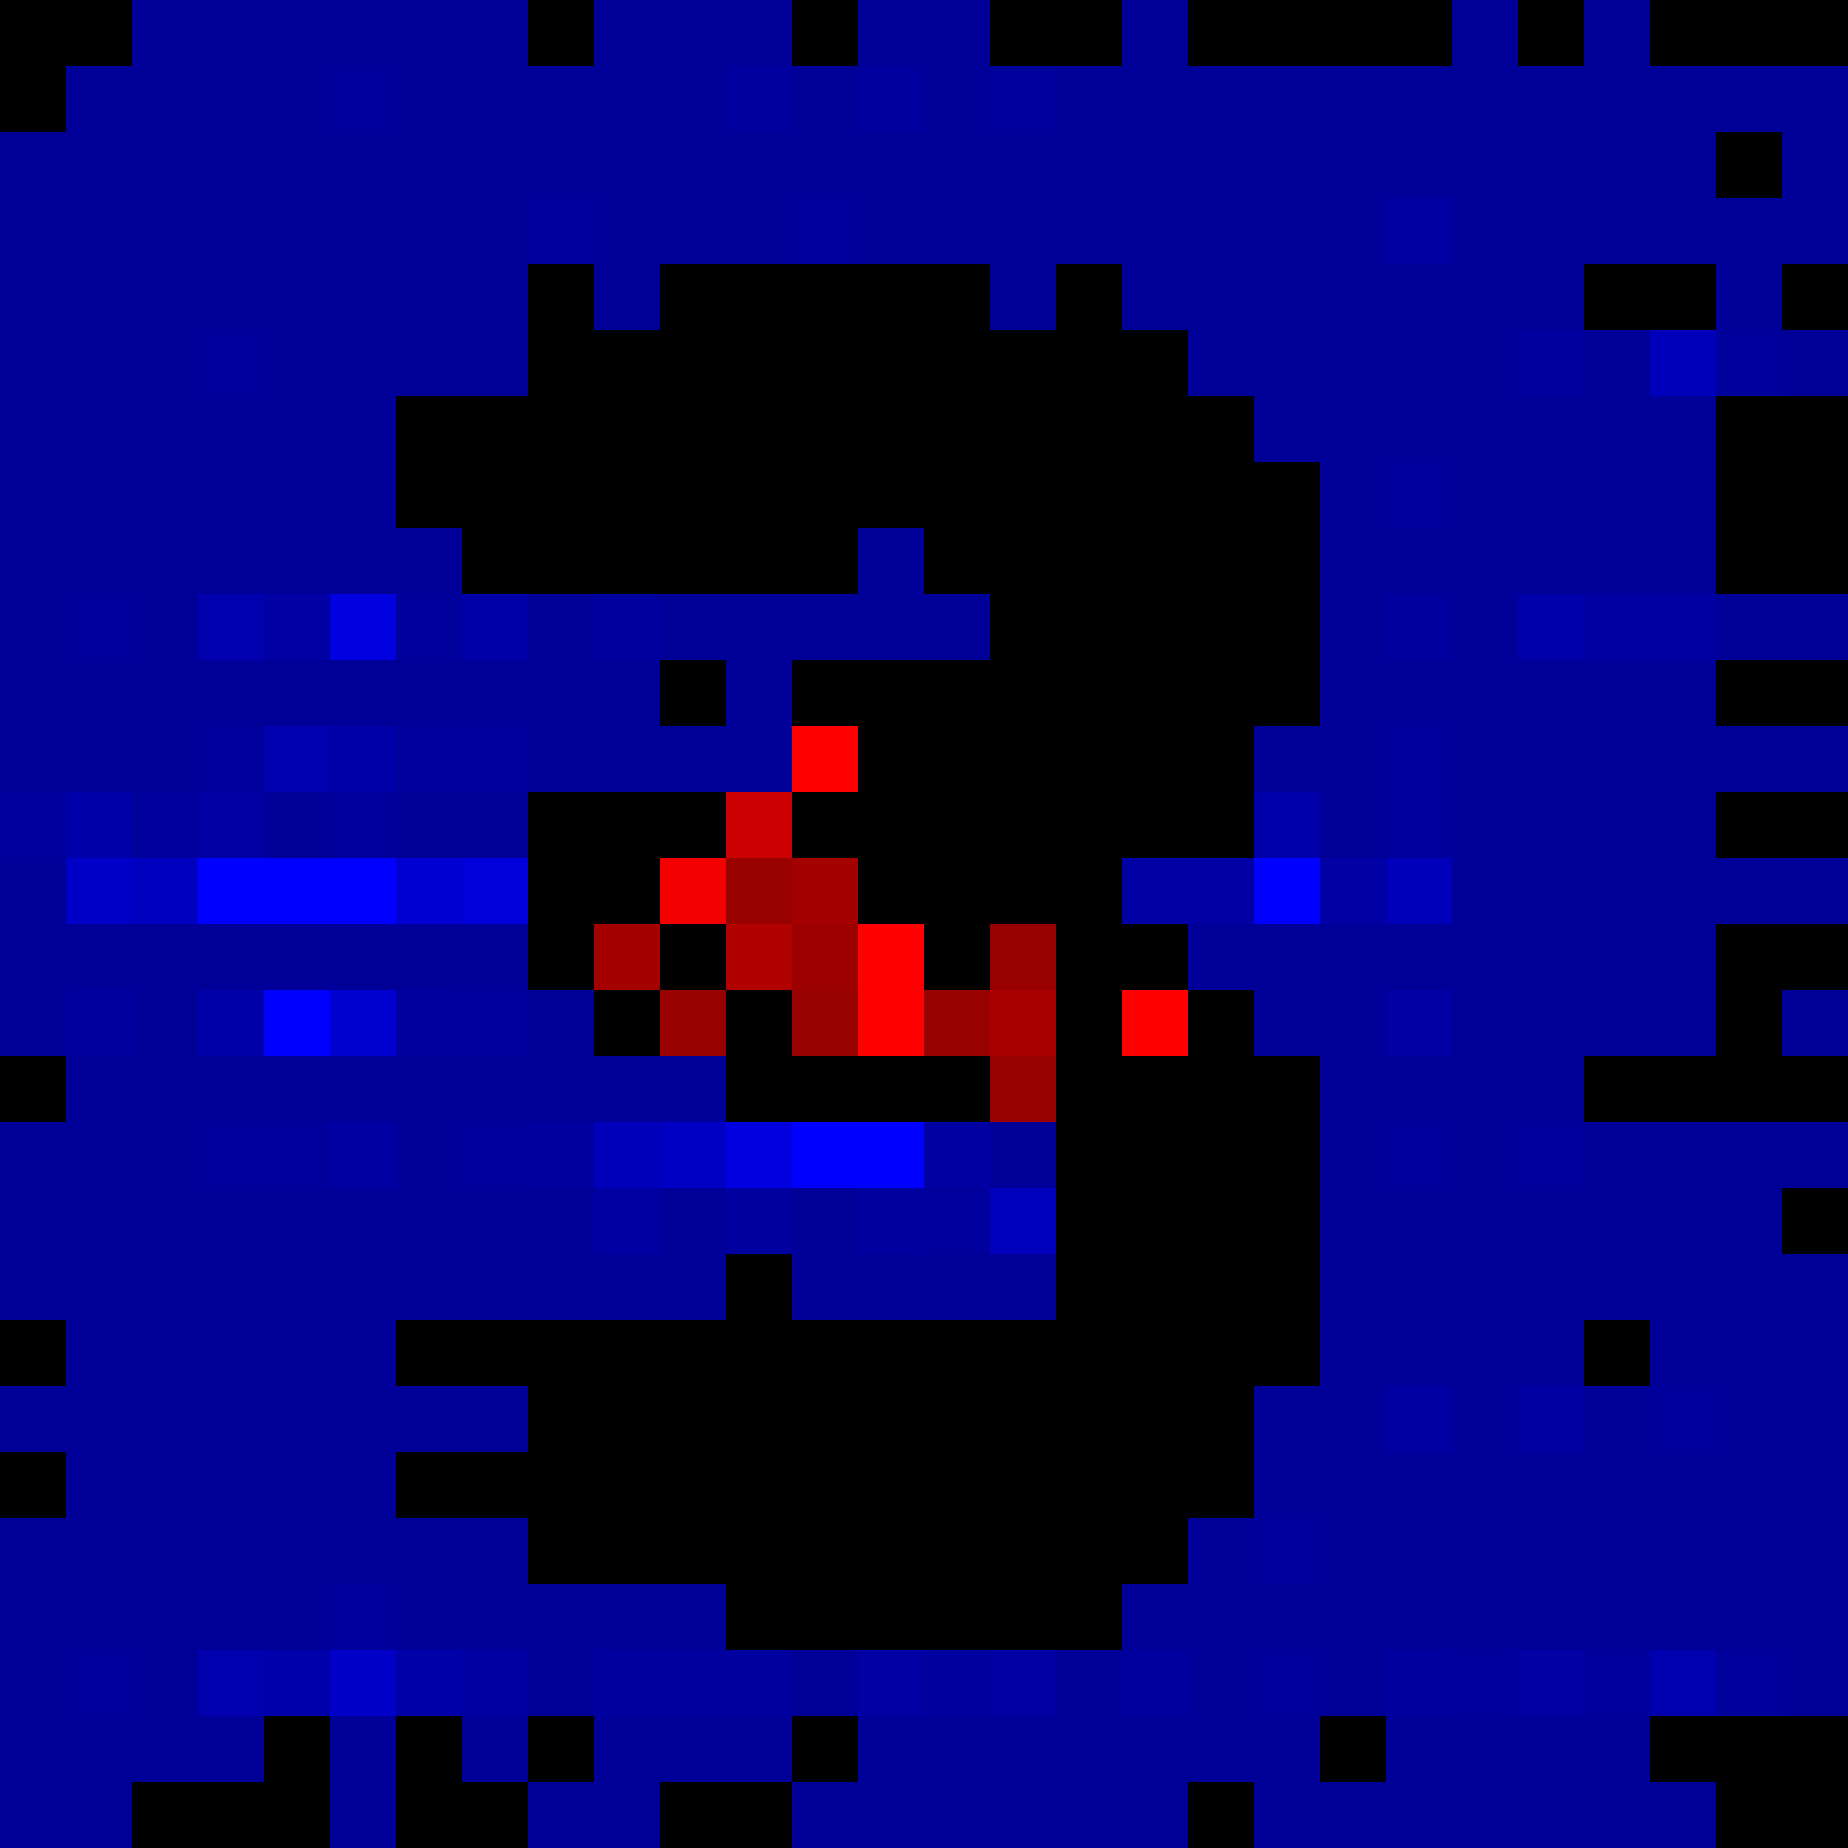
\includegraphics[width=\linewidth]{saliency/mnist_split_ic_saliency/image_036_true_3_pred_3/final_saliency_threshold_wrt_4_bright.png}\\[-1pt]{\scriptsize Logit 4}
		\end{minipage}

		\vspace{0.12cm}

		\begin{minipage}[b]{0.19\linewidth}\centering
			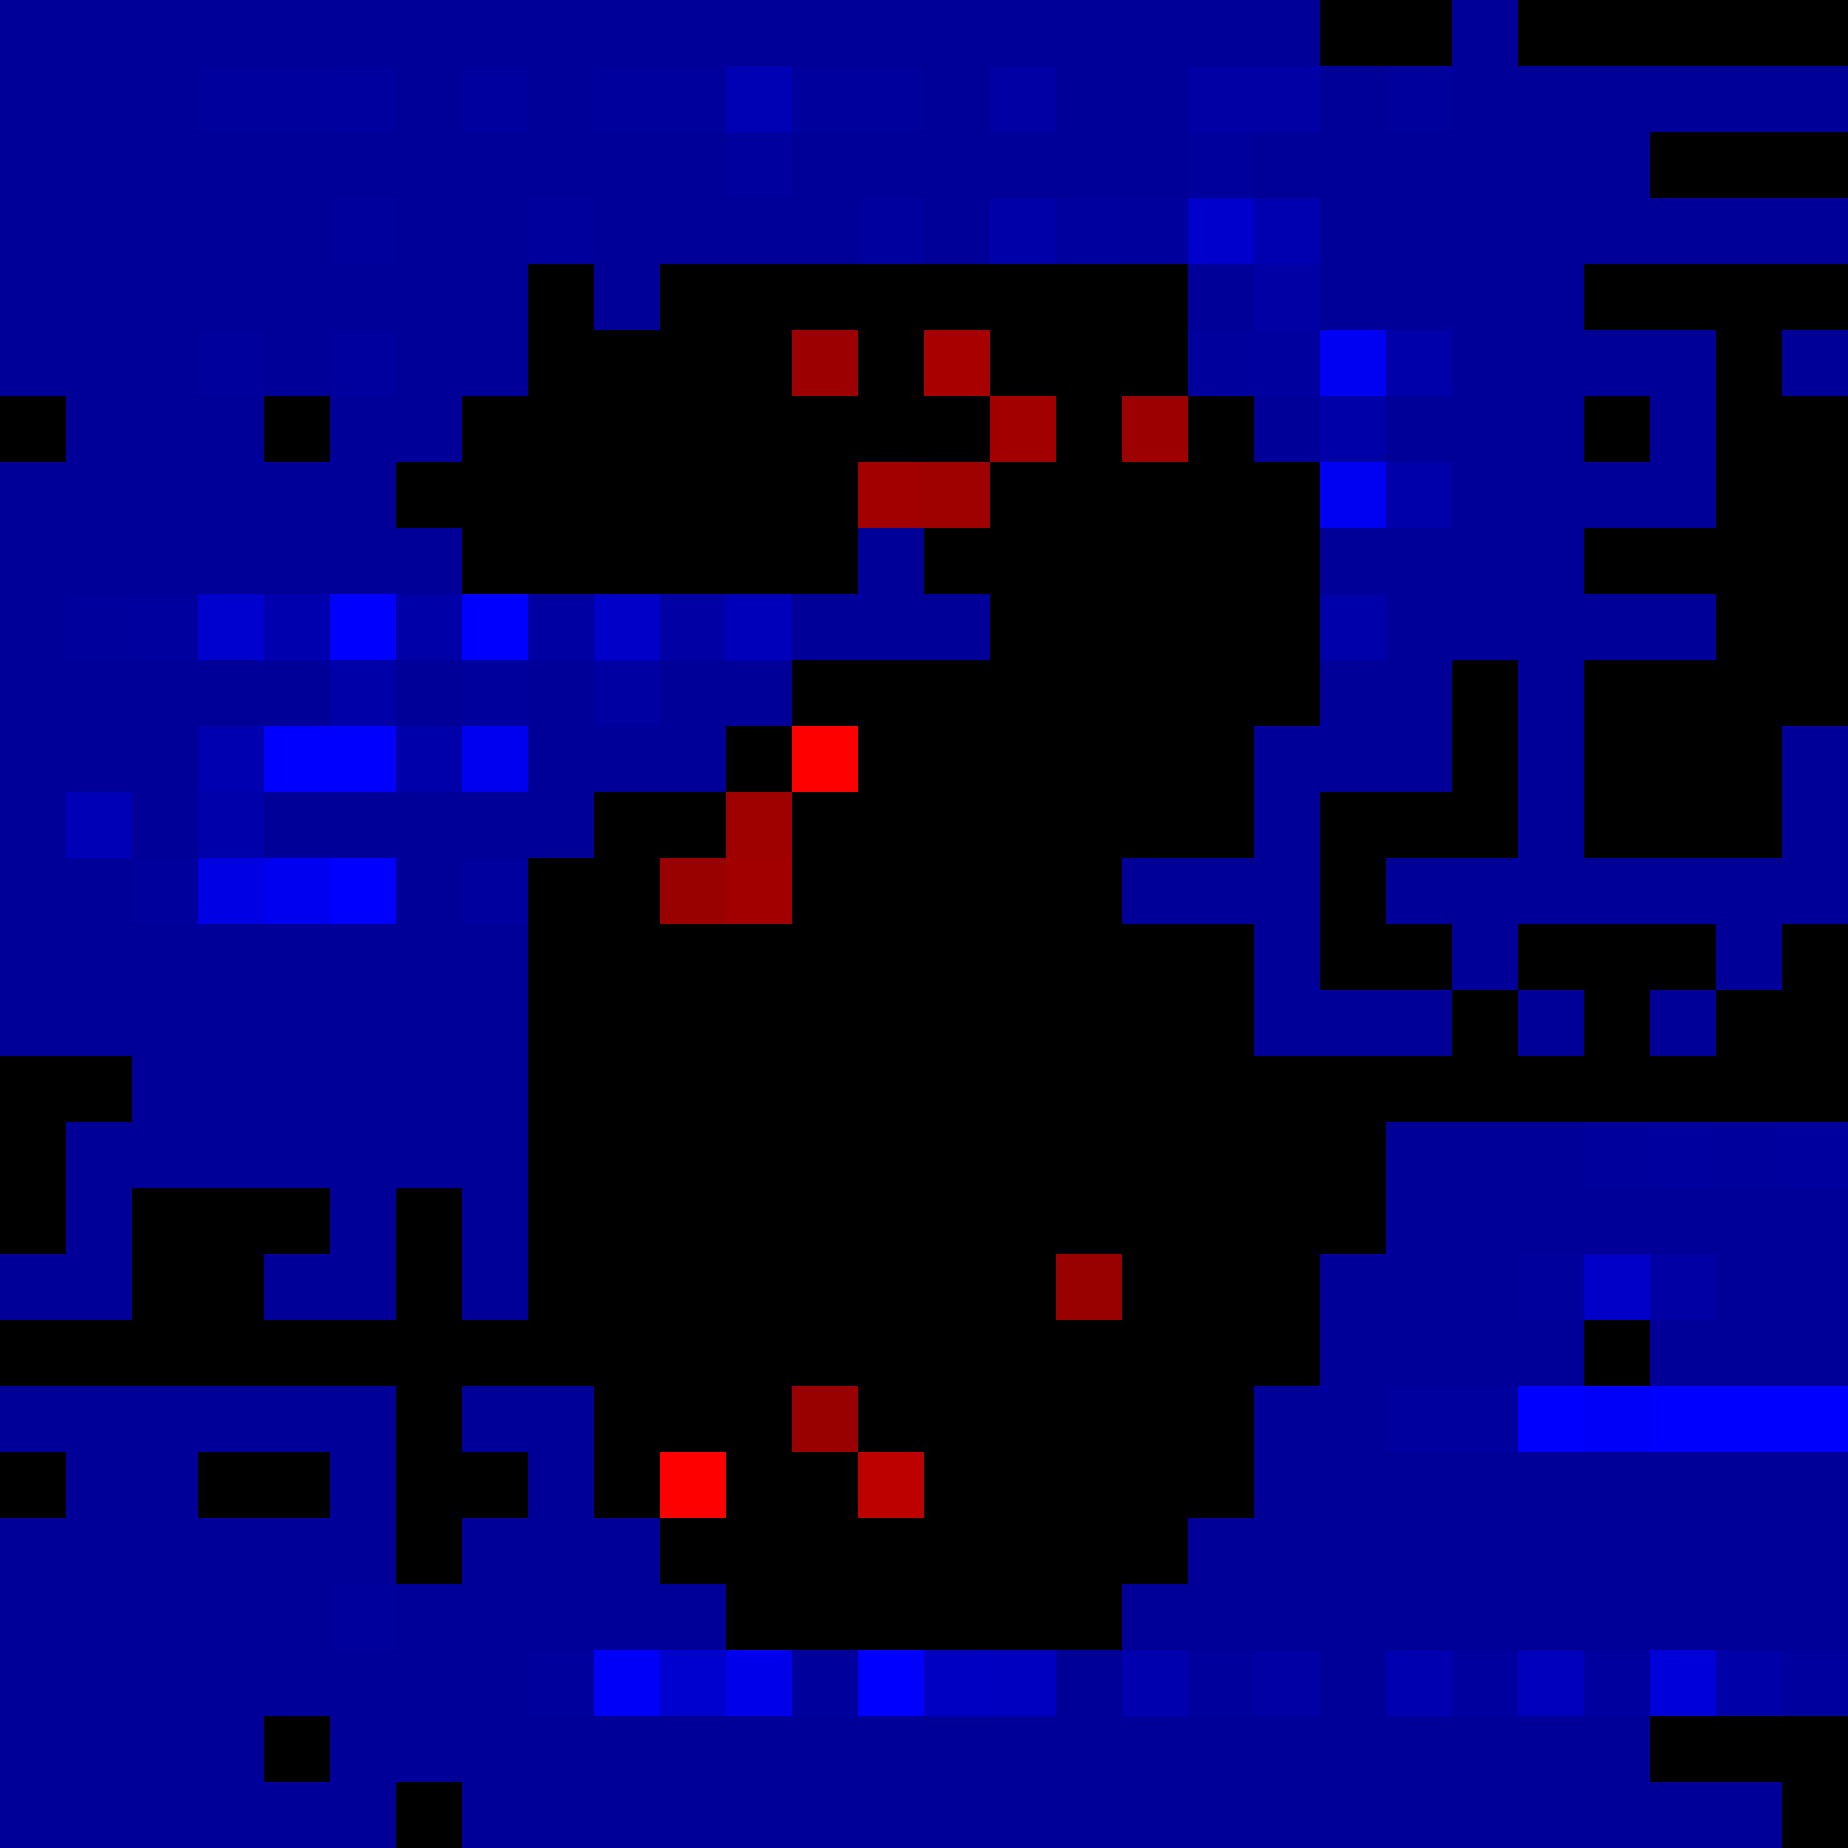
\includegraphics[width=\linewidth]{saliency/mnist_split_ic_saliency/image_036_true_3_pred_3/final_saliency_threshold_wrt_5_bright.png}\\[-1pt]{\scriptsize Logit 5}
		\end{minipage}%
		\begin{minipage}[b]{0.19\linewidth}\centering
			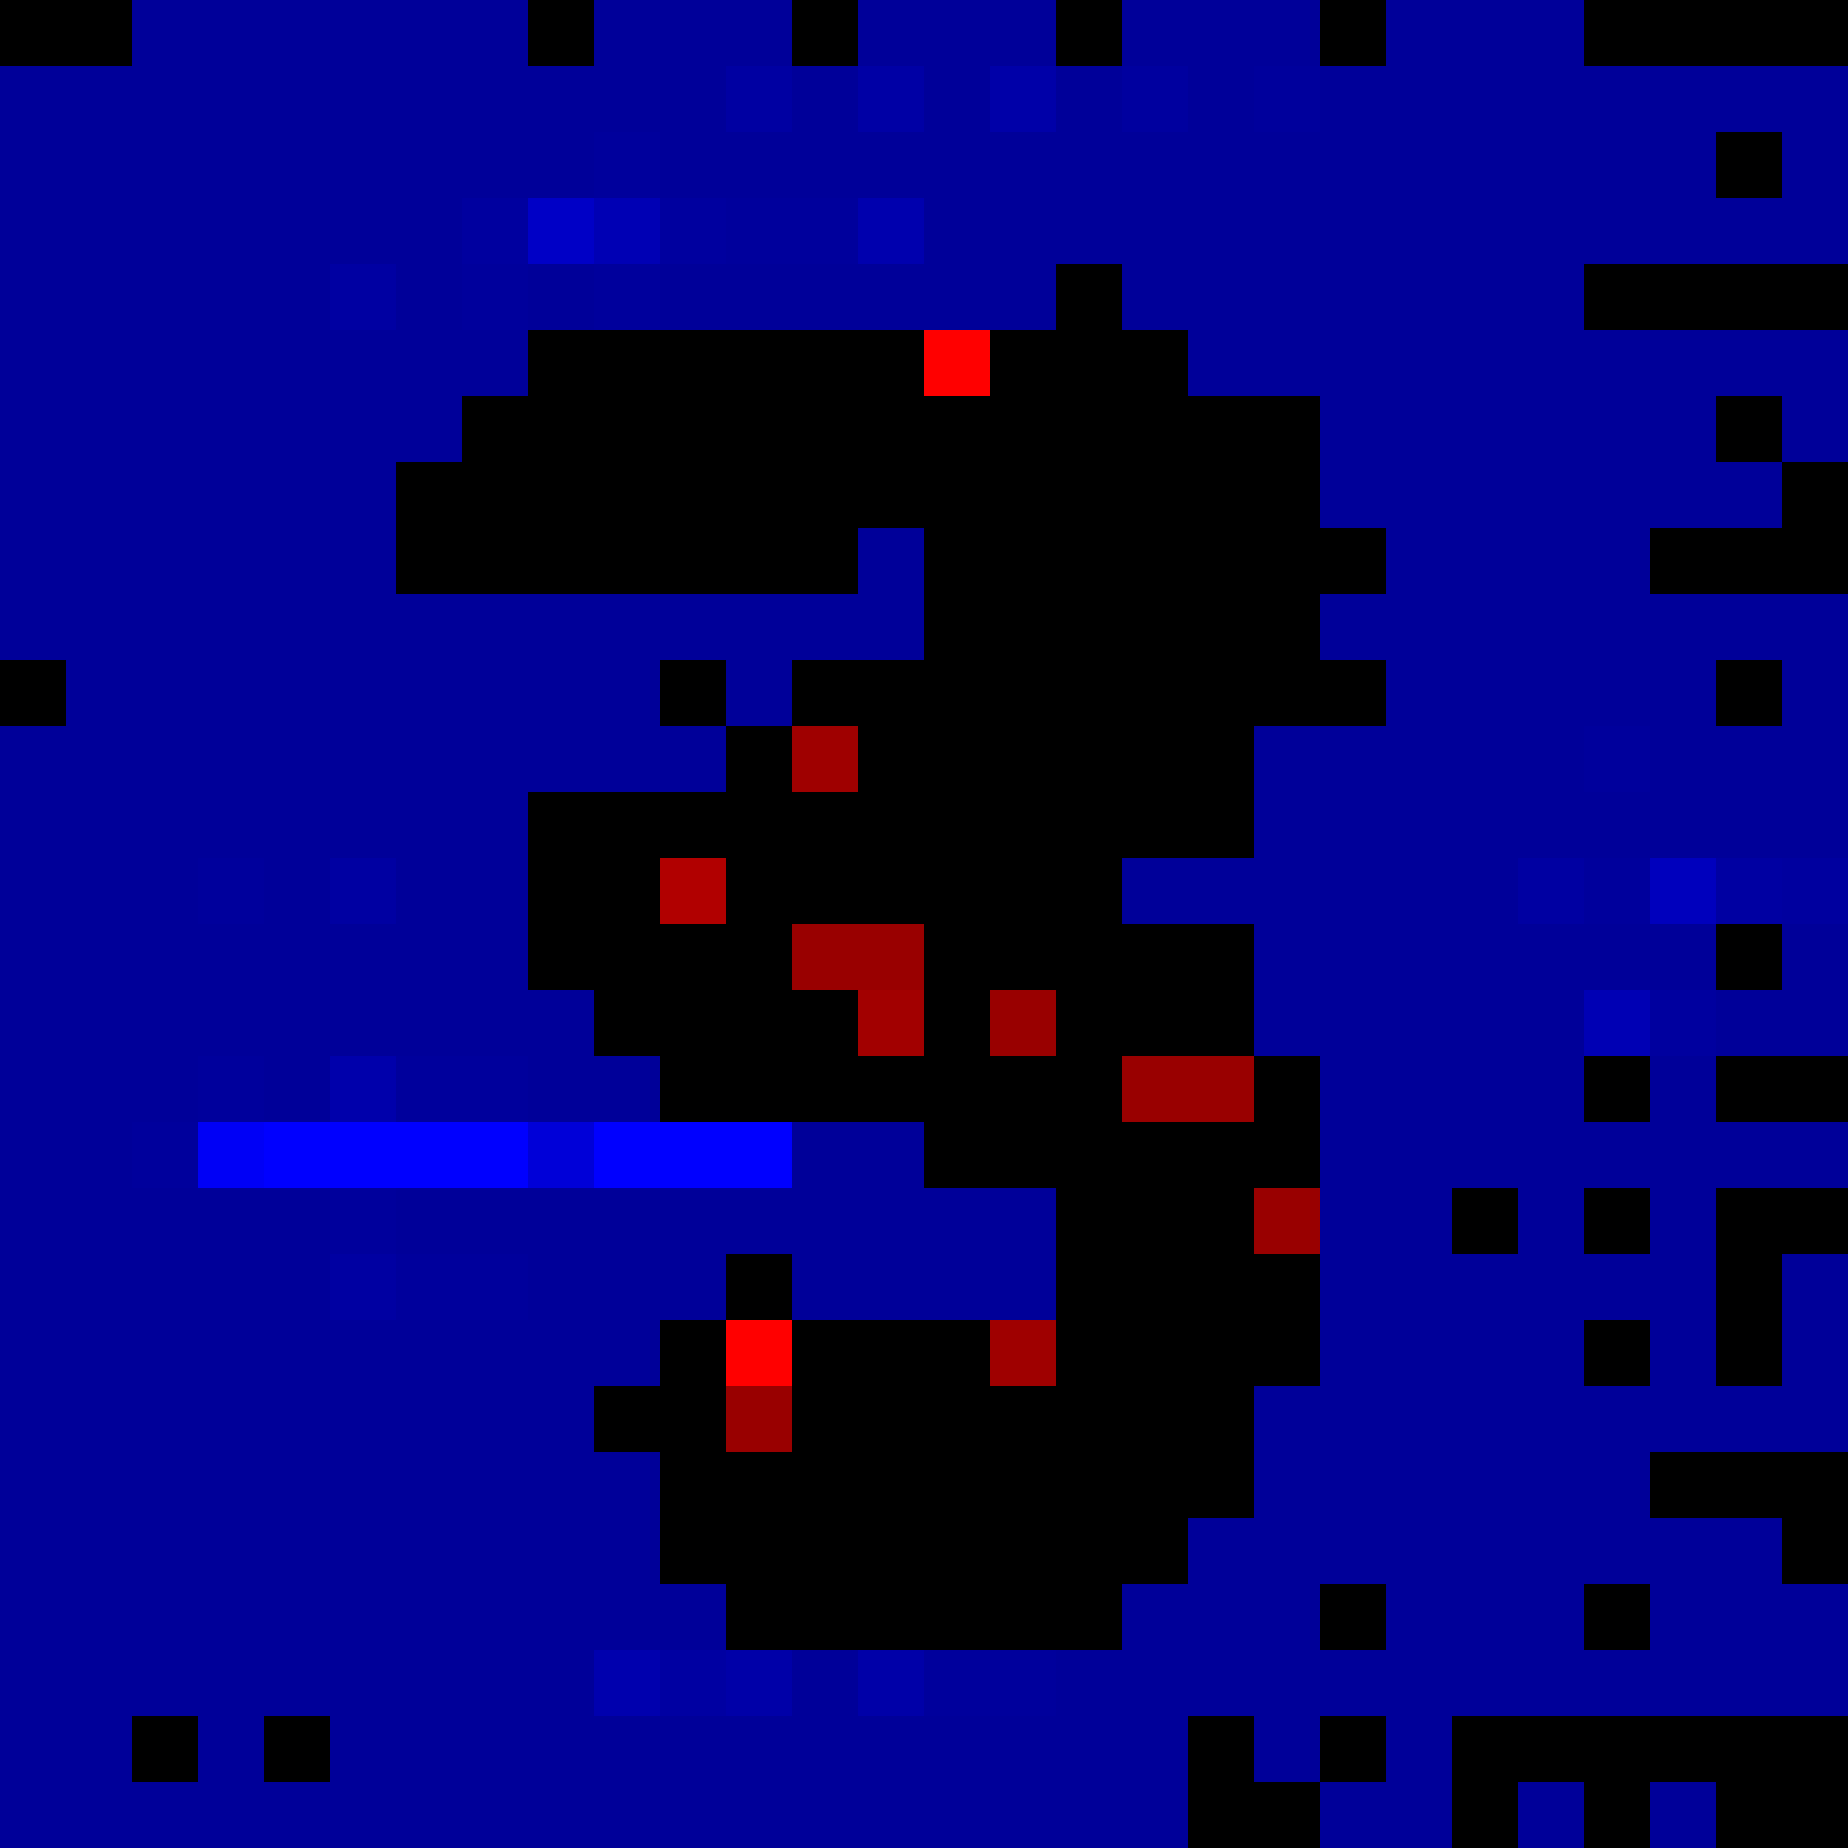
\includegraphics[width=\linewidth]{saliency/mnist_split_ic_saliency/image_036_true_3_pred_3/final_saliency_threshold_wrt_6_bright.png}\\[-1pt]{\scriptsize Logit 6}
		\end{minipage}%
		\begin{minipage}[b]{0.19\linewidth}\centering
			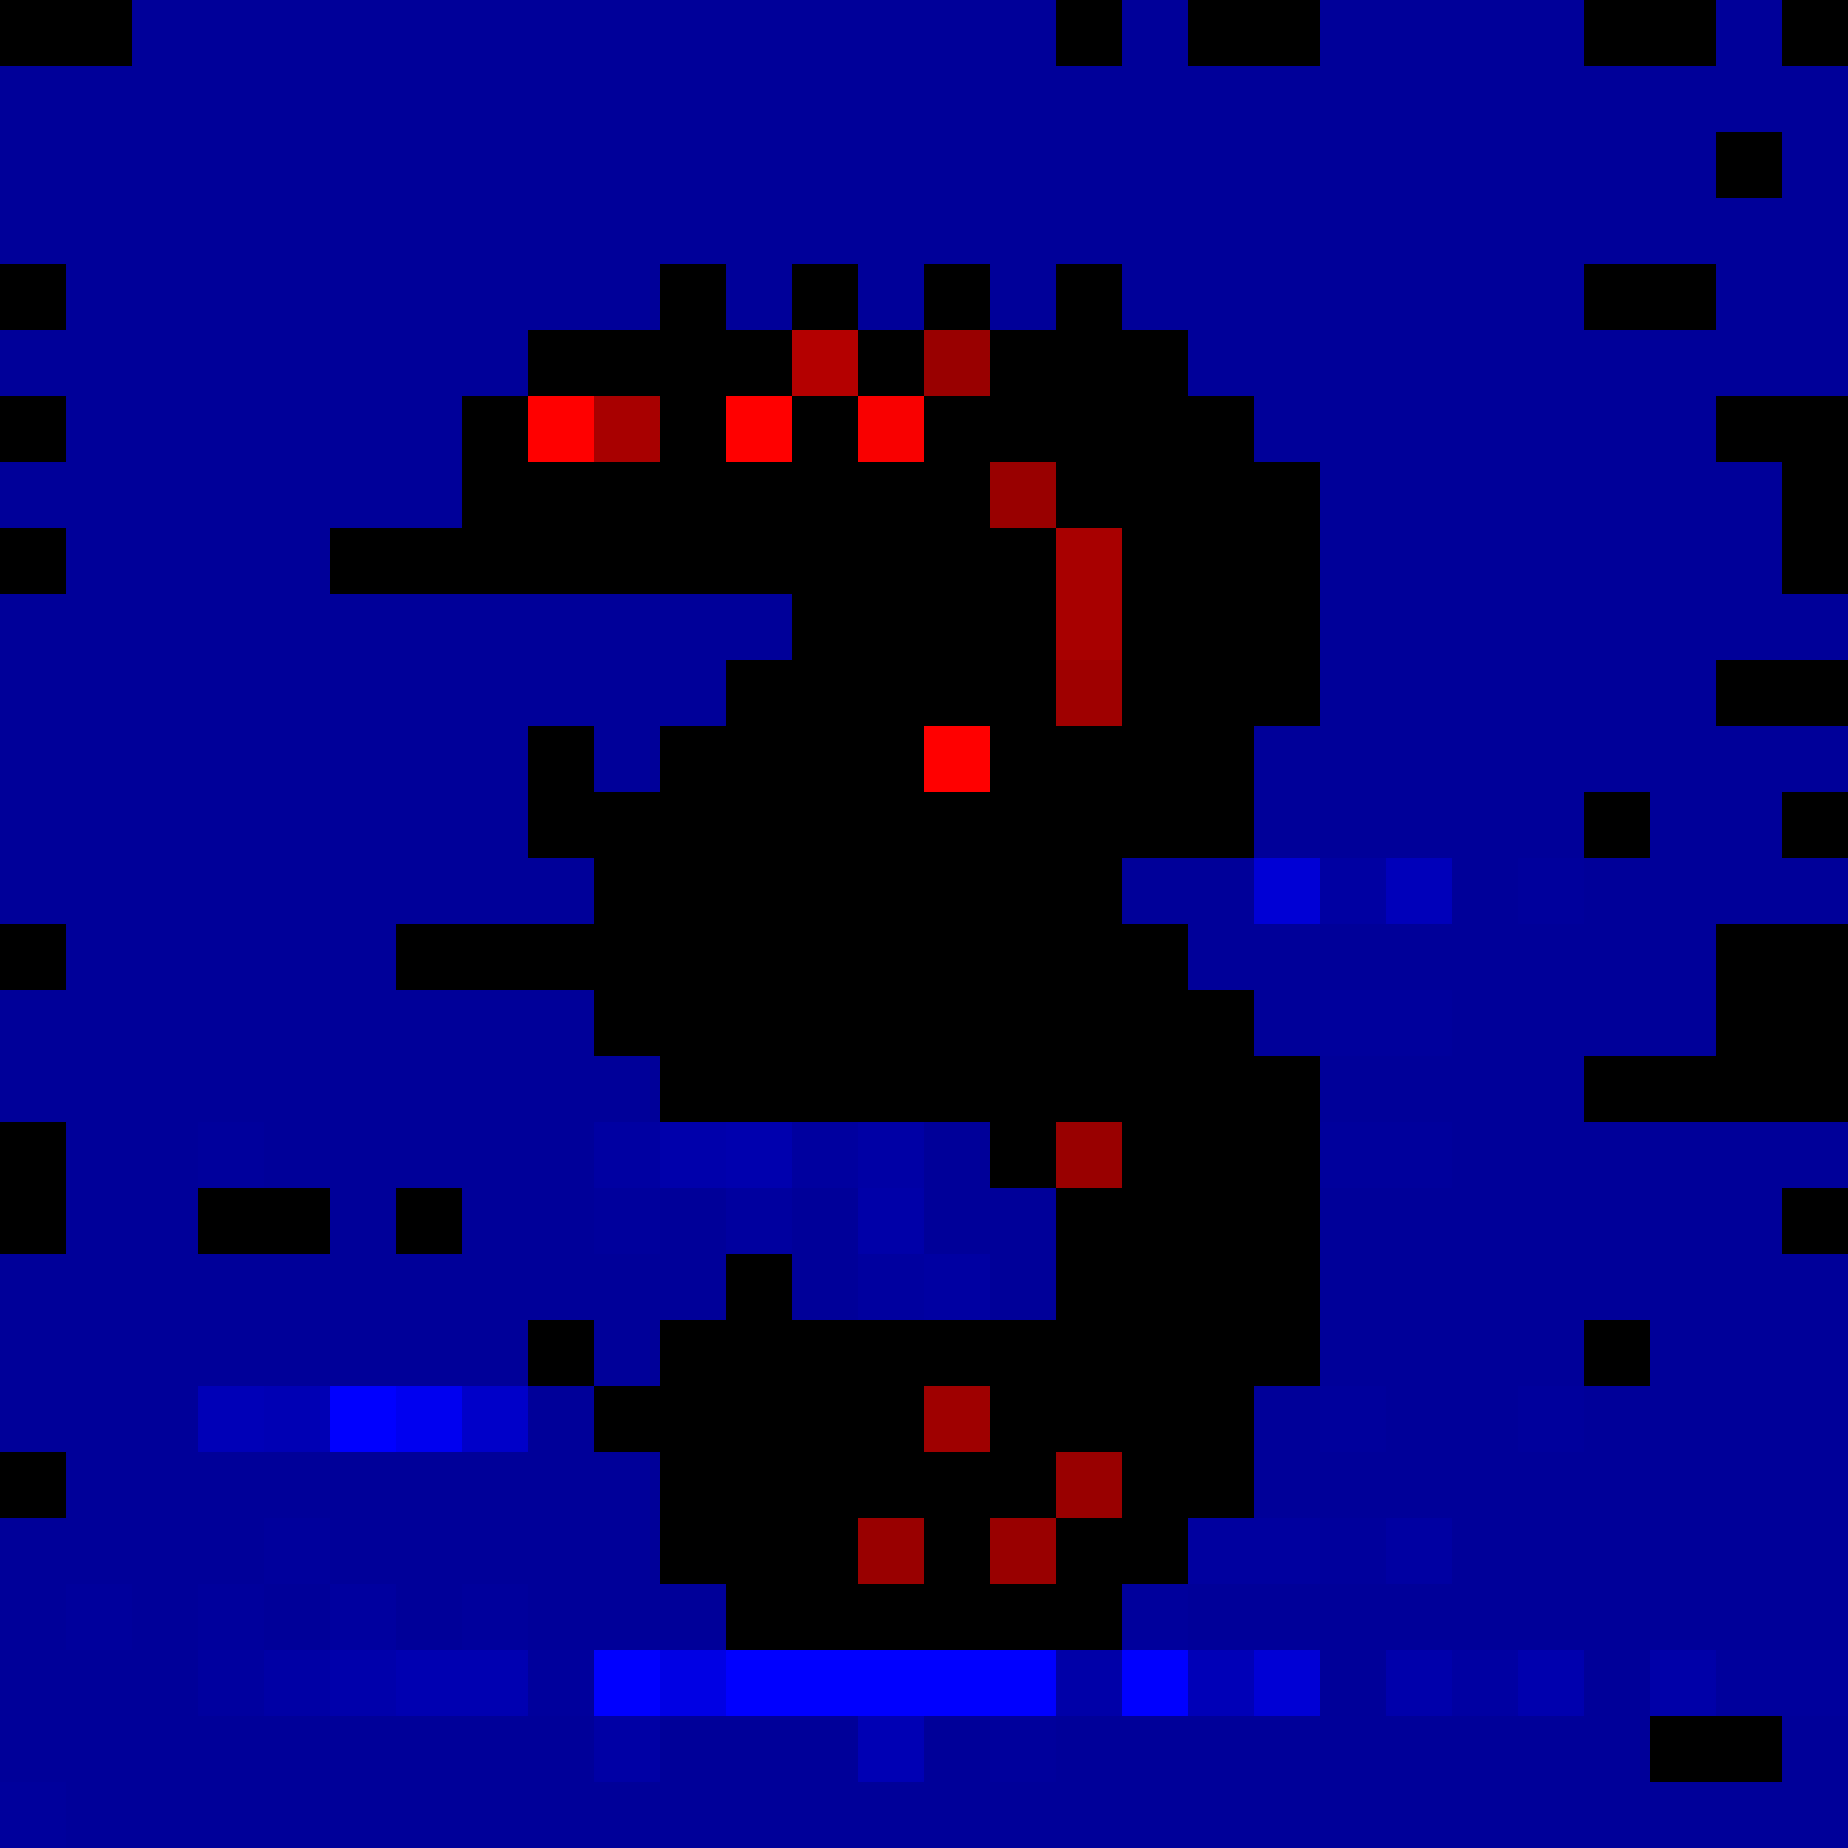
\includegraphics[width=\linewidth]{saliency/mnist_split_ic_saliency/image_036_true_3_pred_3/final_saliency_threshold_wrt_7_bright.png}\\[-1pt]{\scriptsize Logit 7}
		\end{minipage}%
		\begin{minipage}[b]{0.19\linewidth}\centering
			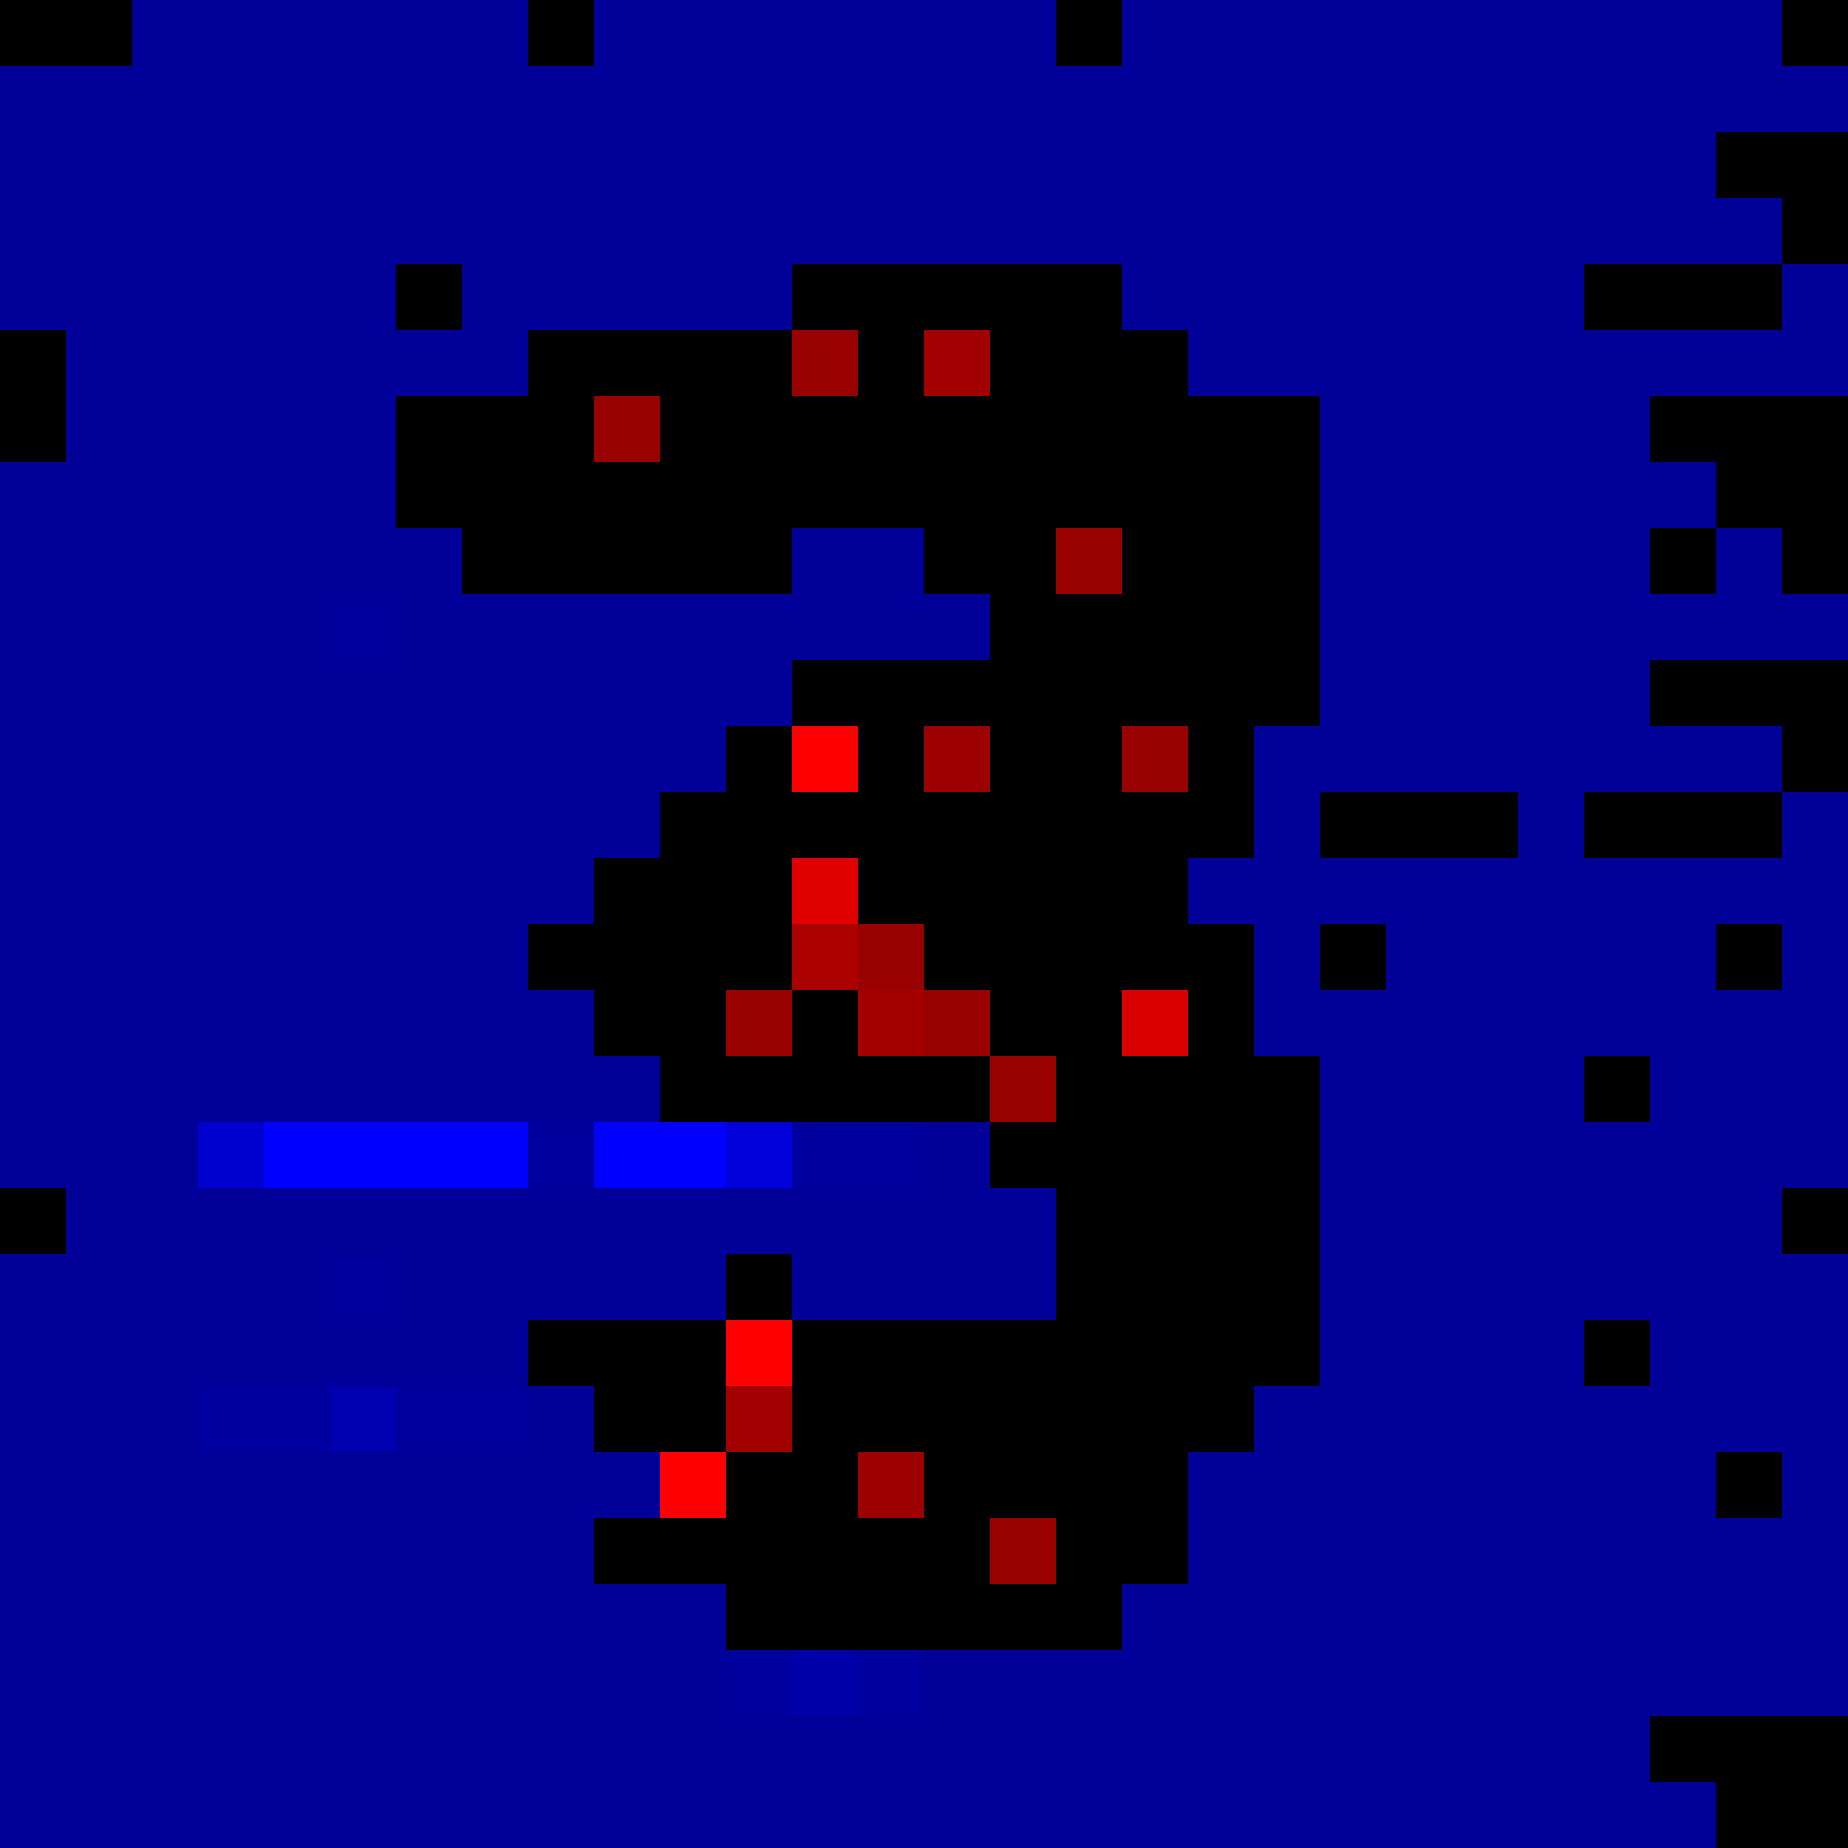
\includegraphics[width=\linewidth]{saliency/mnist_split_ic_saliency/image_036_true_3_pred_3/final_saliency_threshold_wrt_8_bright.png}\\[-1pt]{\scriptsize Logit 8}
		\end{minipage}%
		\begin{minipage}[b]{0.19\linewidth}\centering
			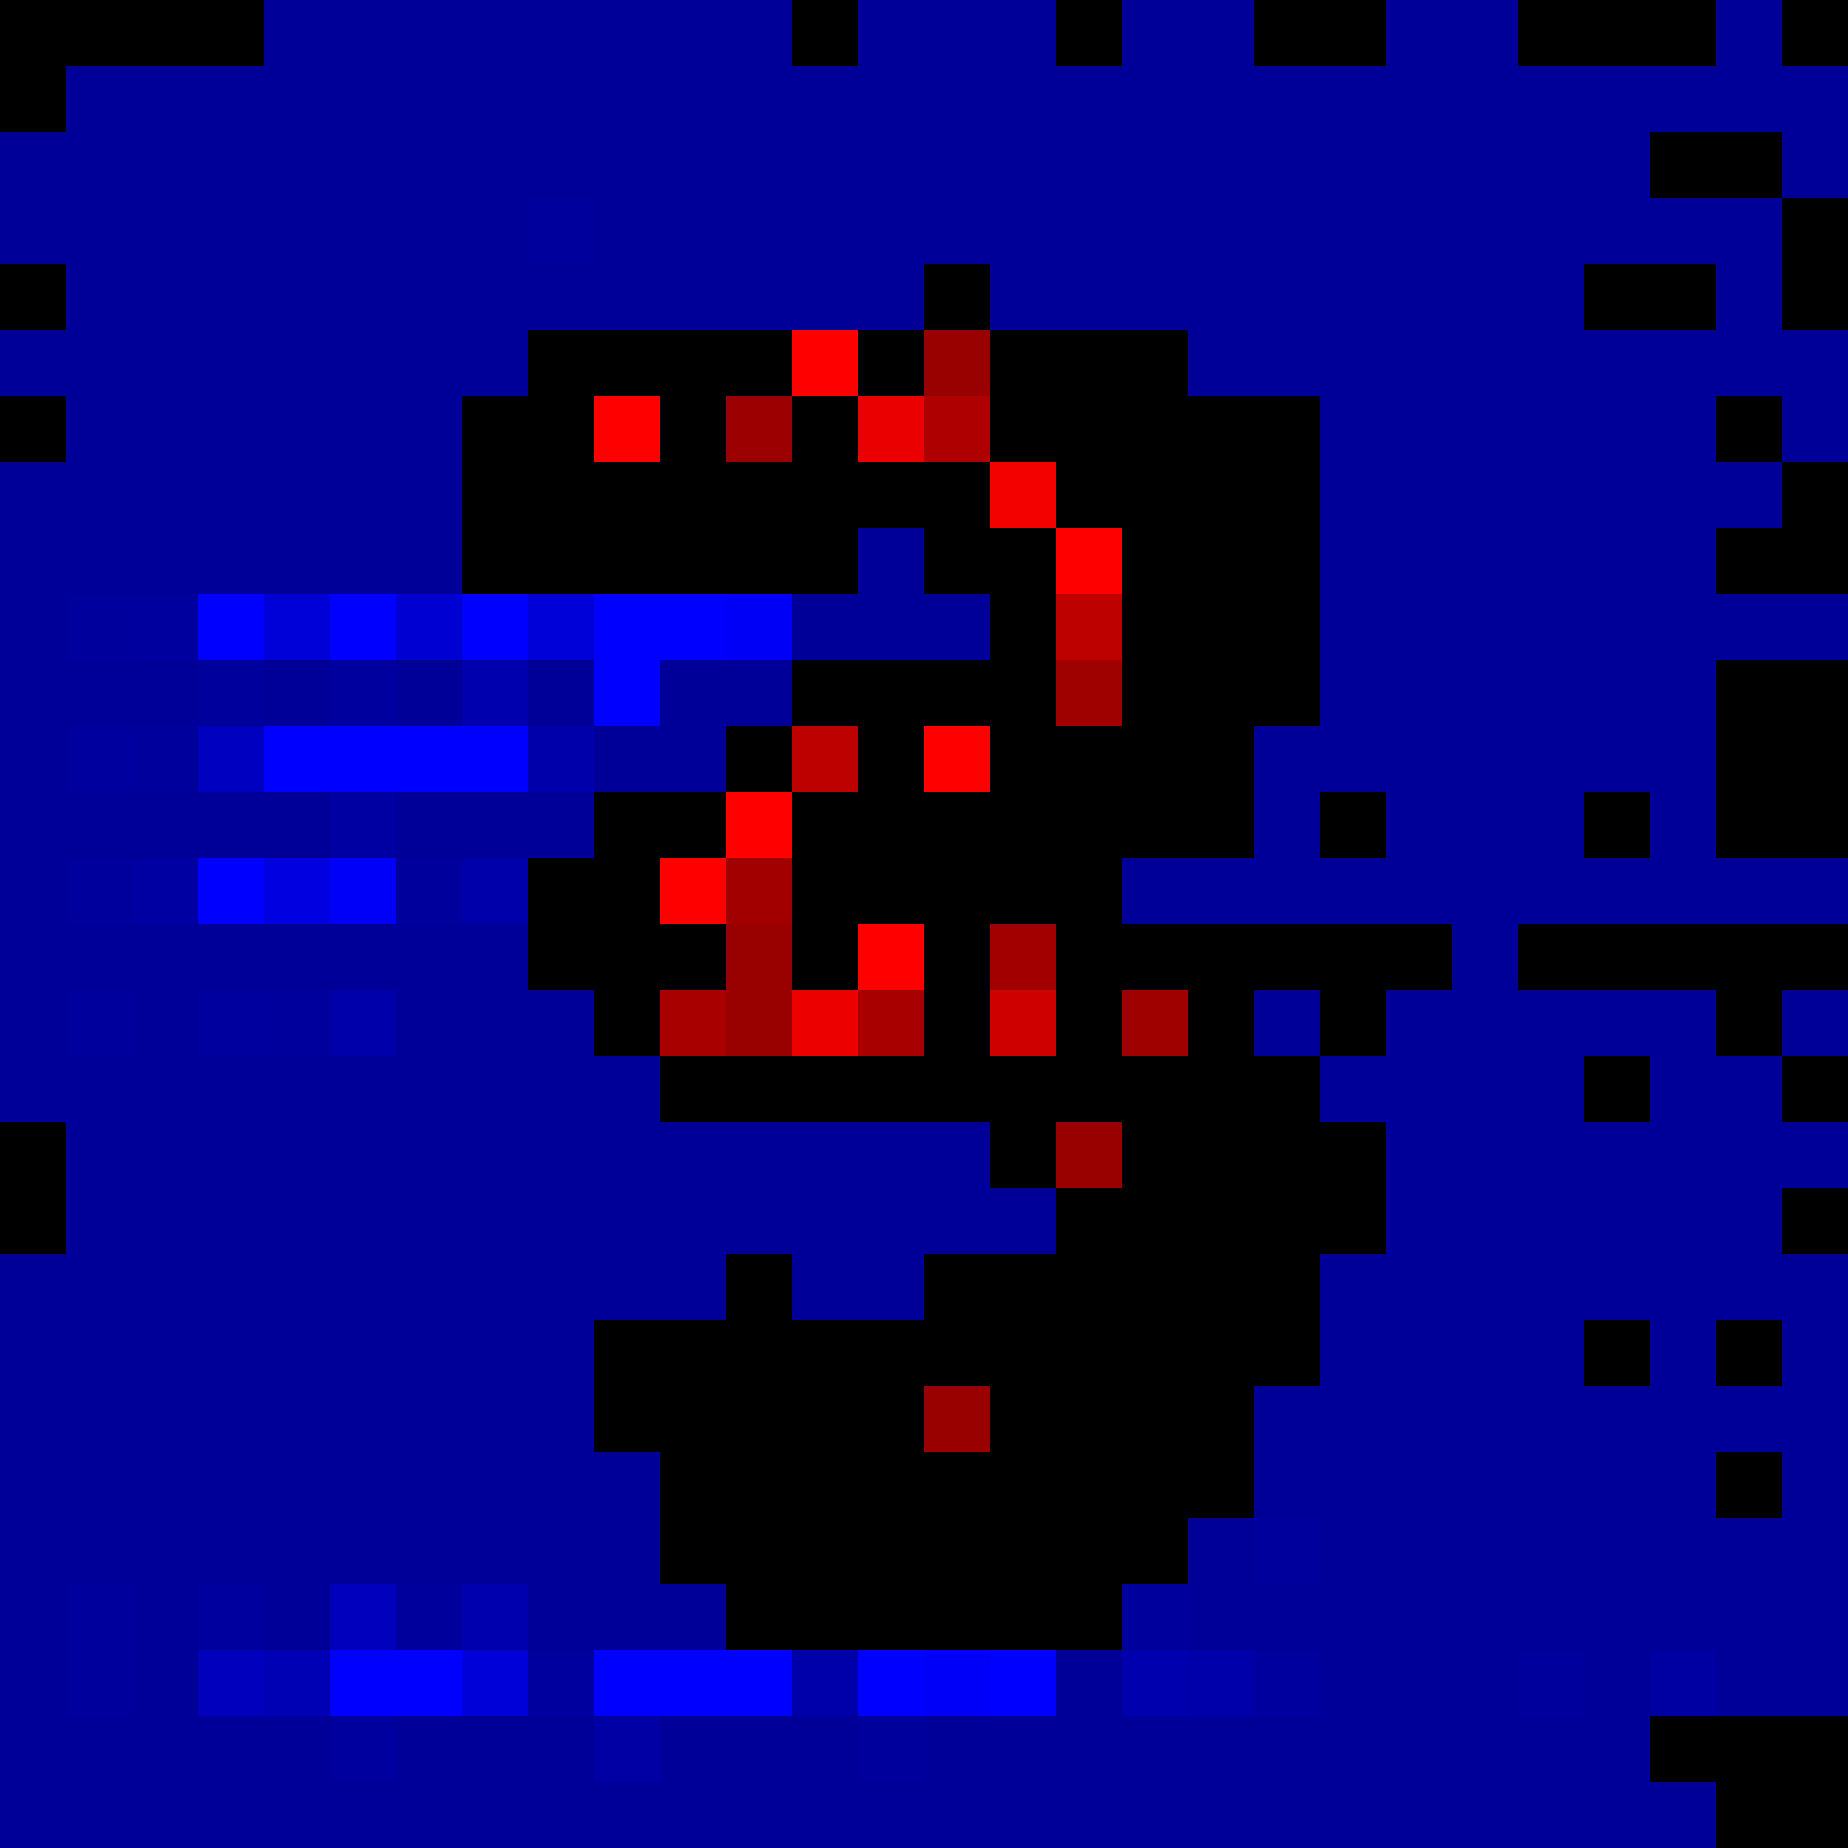
\includegraphics[width=\linewidth]{saliency/mnist_split_ic_saliency/image_036_true_3_pred_3/final_saliency_threshold_wrt_9_bright.png}\\[-1pt]{\scriptsize Logit 9}
		\end{minipage}
	\end{minipage}
	}%
\caption[Second example of inverted-input DIC stream gradients]{Second correctly classified MNIST test ``3'', using the model, per-class thresholded overlays and color convention of Figure~\ref{fig:mnist_split_ic_saliency}. Left: input. These stream-local maps do not by themselves establish the effect of adding pixels on the complete model.}
	\label{fig:mnist_split_ic_saliency_second}
\end{figure}

Figure~\ref{fig:mnist_split_ic_saliency} overlays both gradients for each class logit of a test ``3''. The $g$-gradient best traces strokes for the ground-truth logit; for competing ``6'', ``8'' and ``9'', $h$-gradients concentrate \emph{between the arches}, where added pixels would geometrically close loops. A second correctly classified ``3'' (Figure~\ref{fig:mnist_split_ic_saliency_second}) shows the same qualitative pattern. The single \texttt{cnn\_maxout} IC model's gradients are mostly positive on strokes and negative on background, with less class-dependent directional variation. These examples suggest a role for the difference structure without establishing general disentanglement.

\paragraph{Qualitative comparison with a single input-convex model.}
Figure~\ref{fig:mnist_ic_saliency} reproduces the source paper's ten-class input-gradient comparison for the single \texttt{cnn\_maxout} IC model, showing the stroke/background sign pattern described above. Together with the class-dependent DICIN maps (Figures~\ref{fig:mnist_split_ic_saliency},~\ref{fig:mnist_split_ic_saliency_second}), it motivates a factual/counterfactual reading; finite-intervention effects and separation across all inputs and models require further tests.

\begin{figure}[t]
\QualitativeImageContent{
    \centering
    \begin{minipage}[b]{0.09\linewidth}\centering
        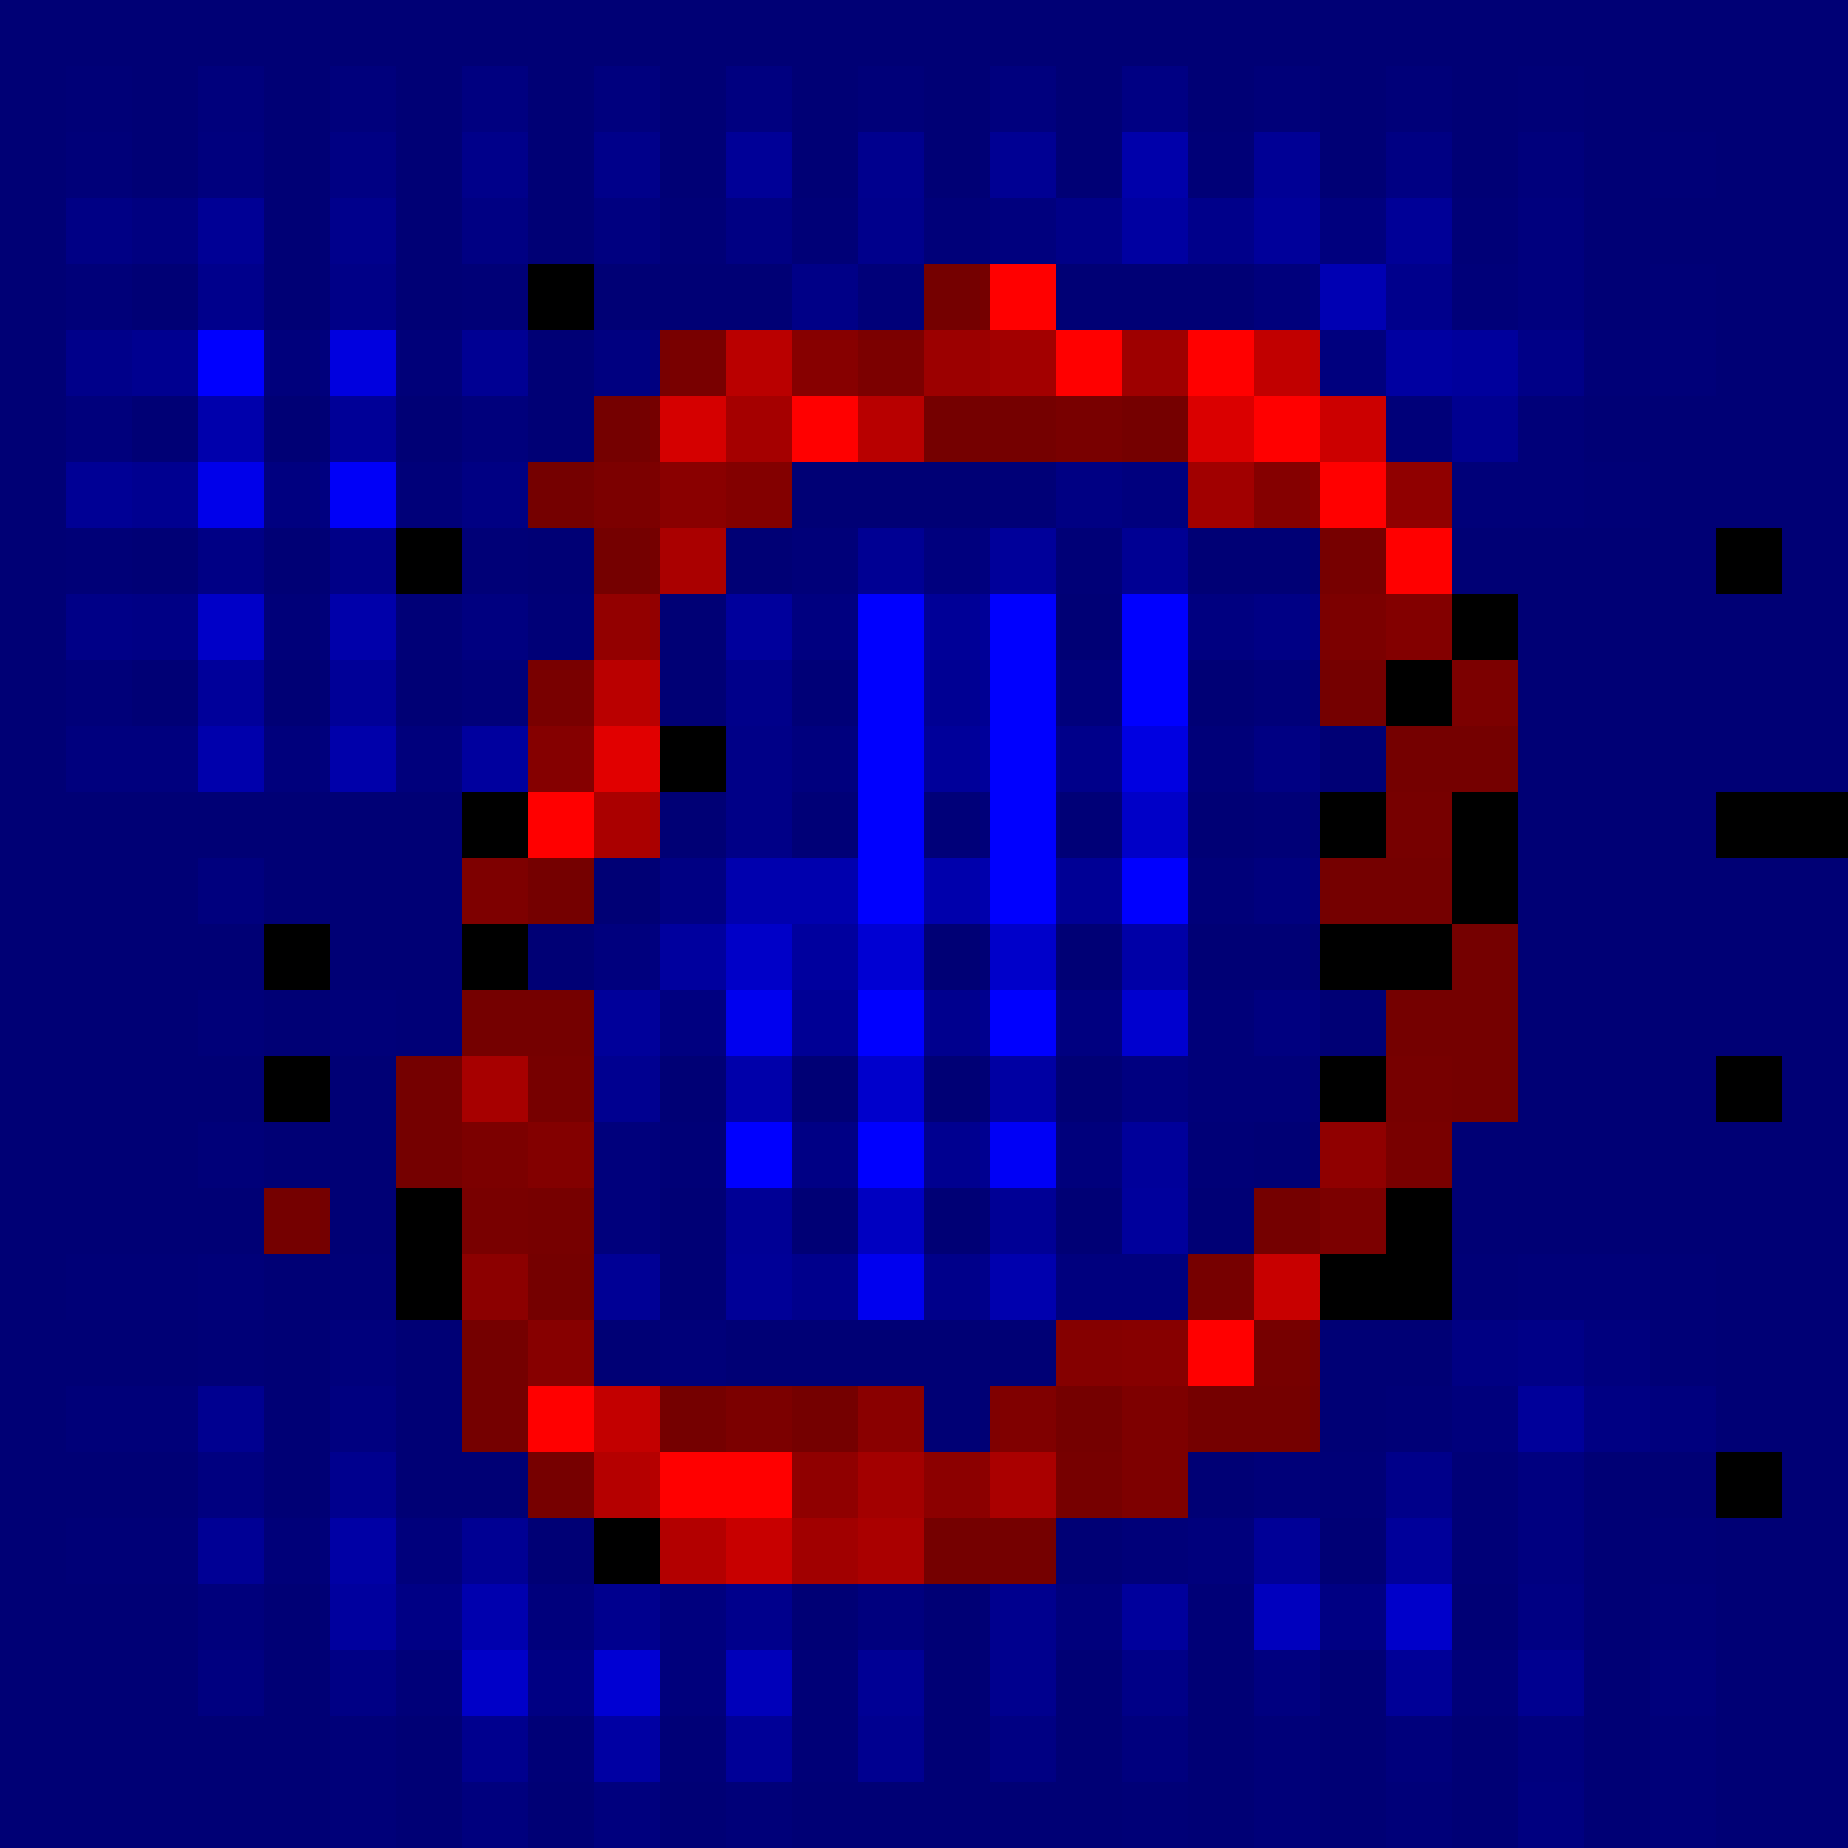
\includegraphics[width=\linewidth]{saliency/mnist_ic_saliency/saliency_threshold_wrt_0_bright.png}
        \scriptsize Gradient 0
    \end{minipage}%
    \begin{minipage}[b]{0.09\linewidth}\centering
        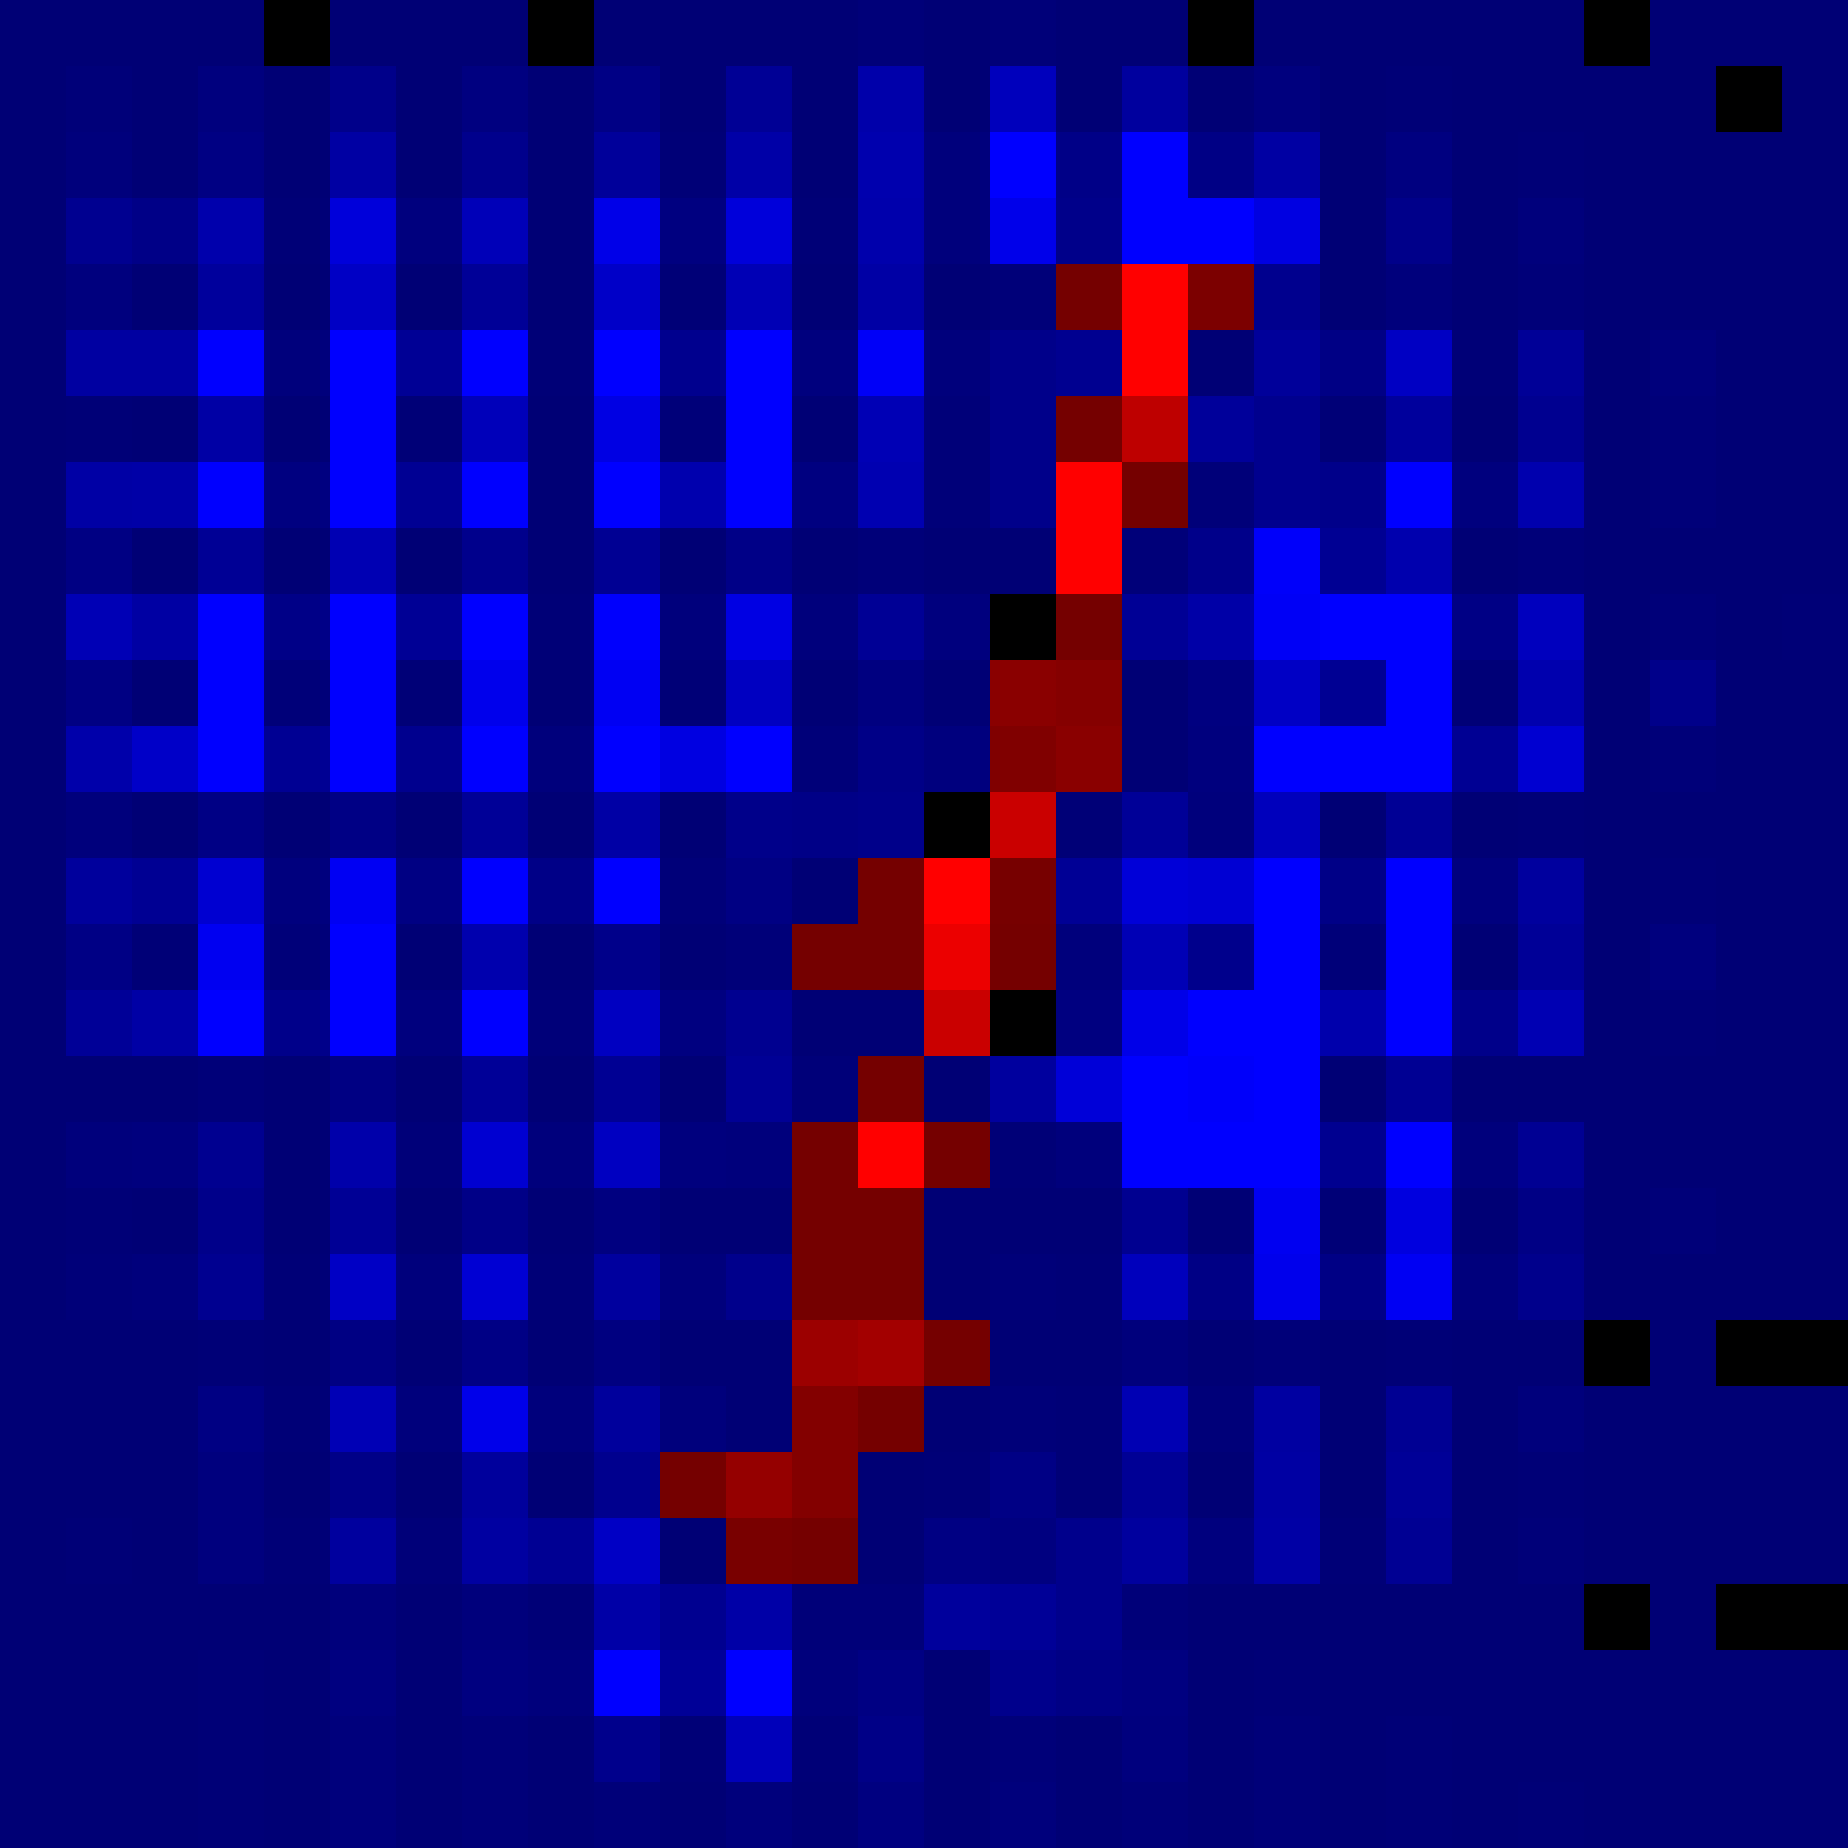
\includegraphics[width=\linewidth]{saliency/mnist_ic_saliency/saliency_threshold_wrt_1_bright.png}
        \scriptsize Gradient 1
    \end{minipage}%
    \begin{minipage}[b]{0.09\linewidth}\centering
        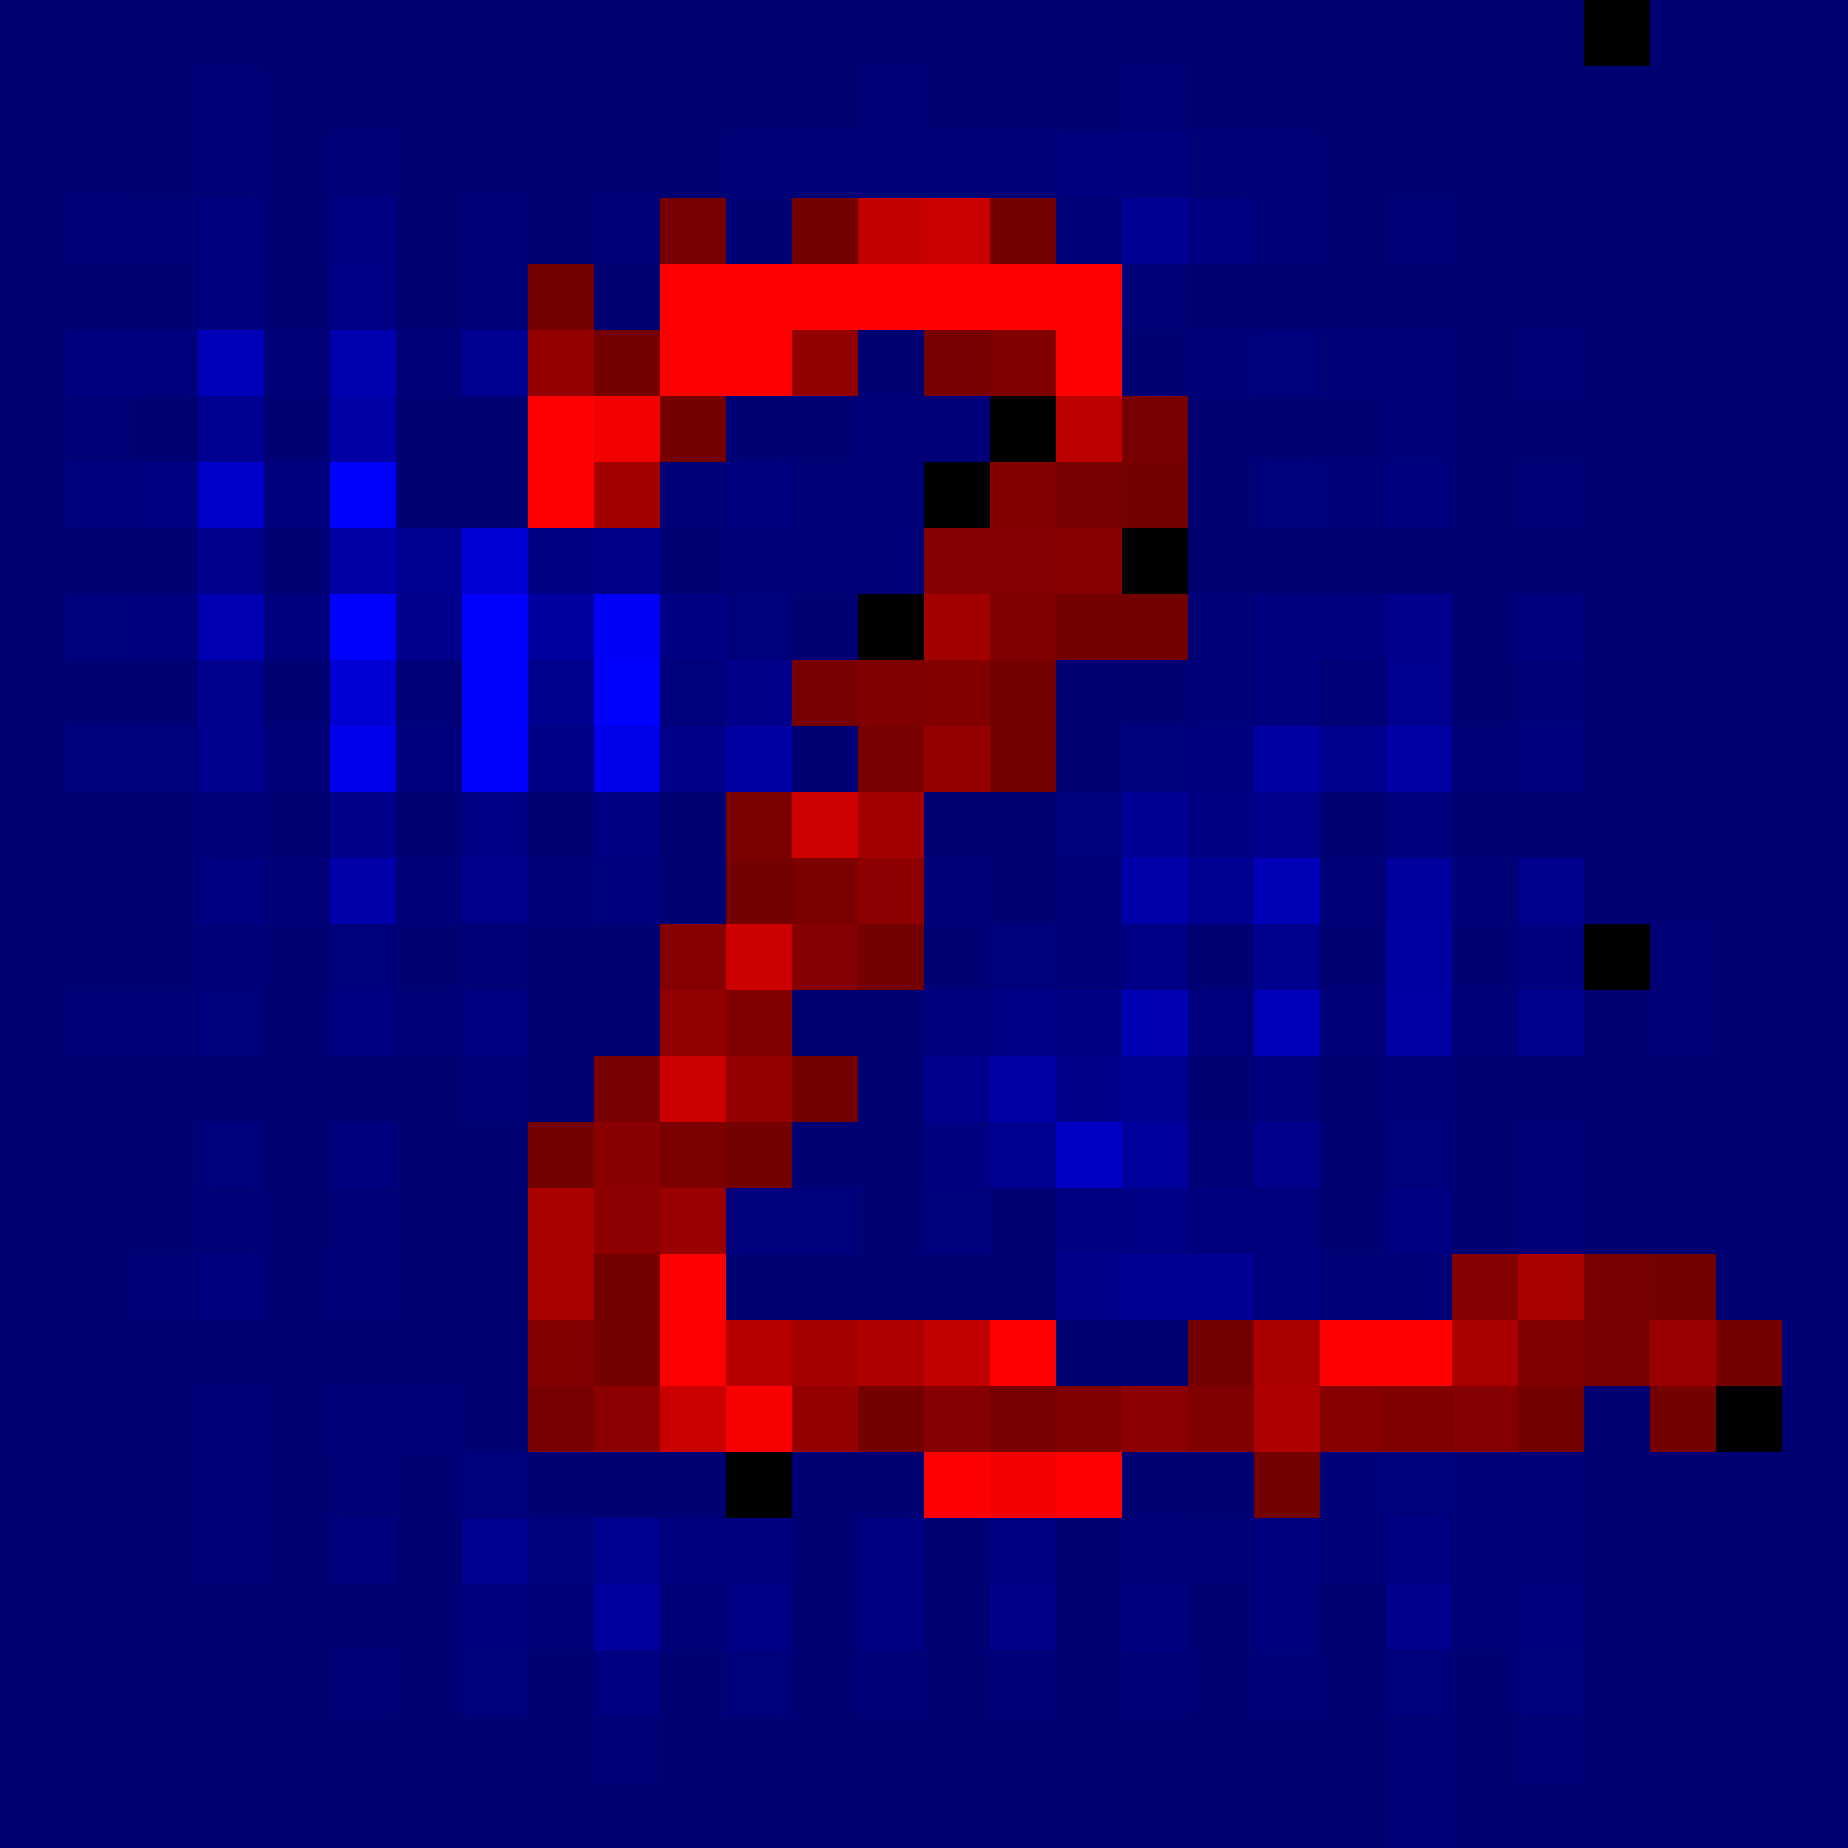
\includegraphics[width=\linewidth]{saliency/mnist_ic_saliency/saliency_threshold_wrt_2_bright.png}
        \scriptsize Gradient 2
    \end{minipage}%
    \begin{minipage}[b]{0.09\linewidth}\centering
        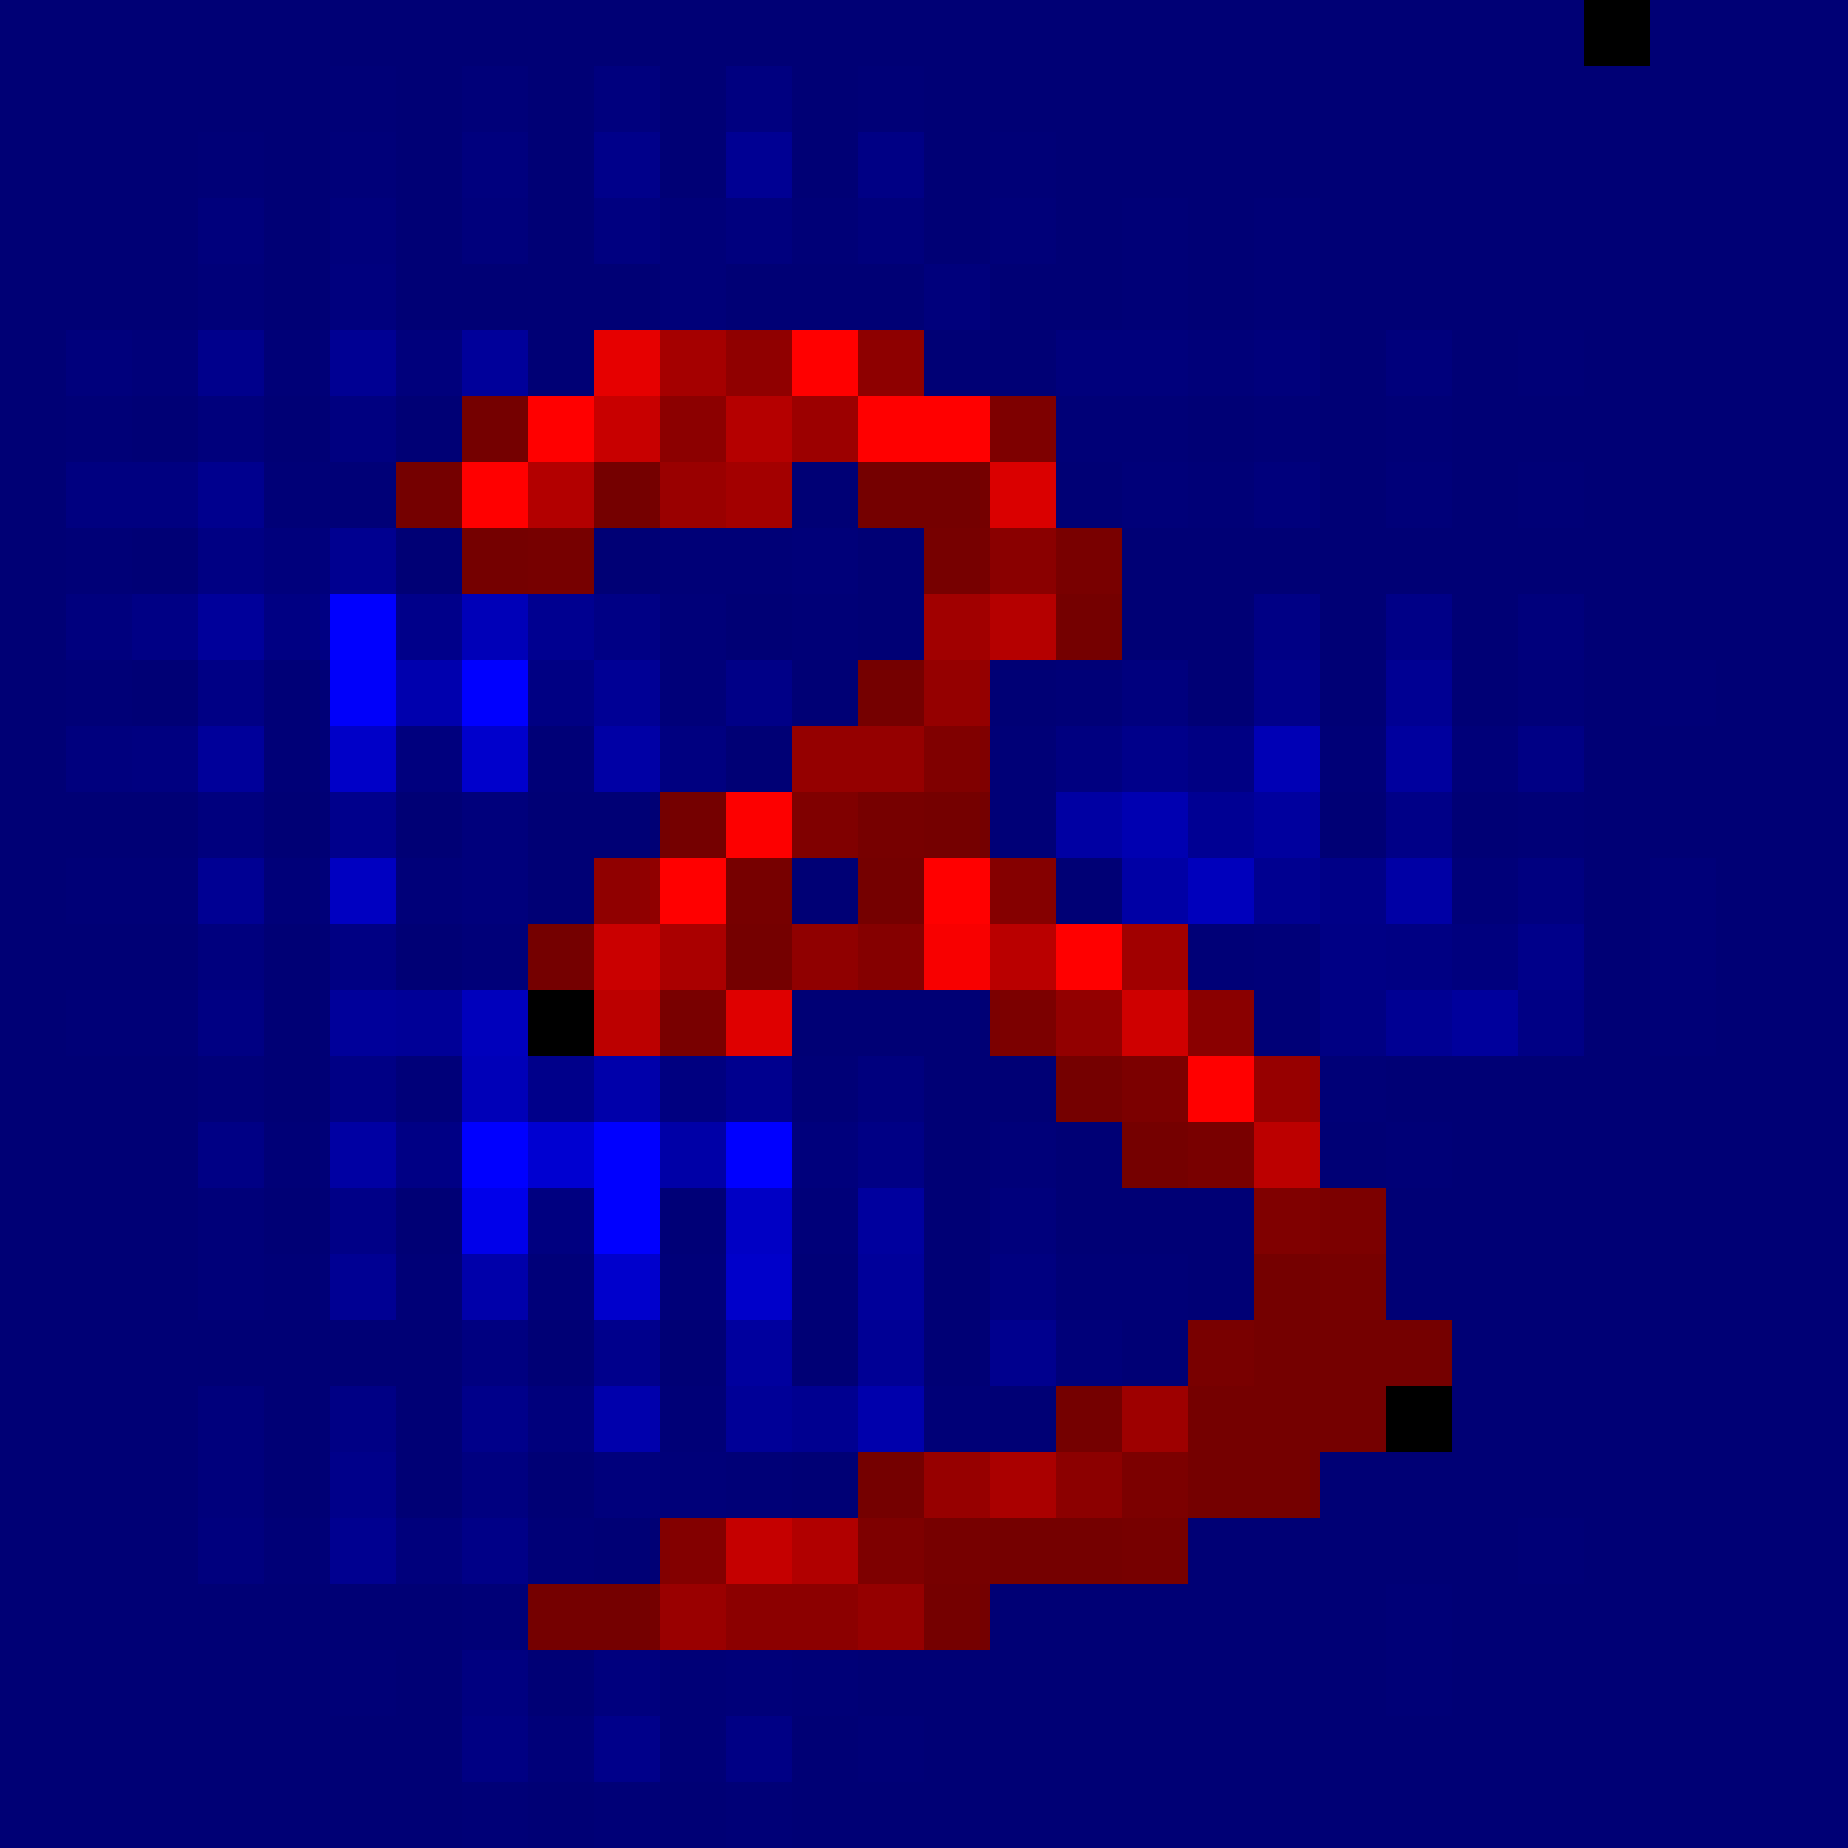
\includegraphics[width=\linewidth]{saliency/mnist_ic_saliency/saliency_threshold_wrt_3_bright.png}
        \scriptsize Gradient 3
    \end{minipage}%
    \begin{minipage}[b]{0.09\linewidth}\centering
        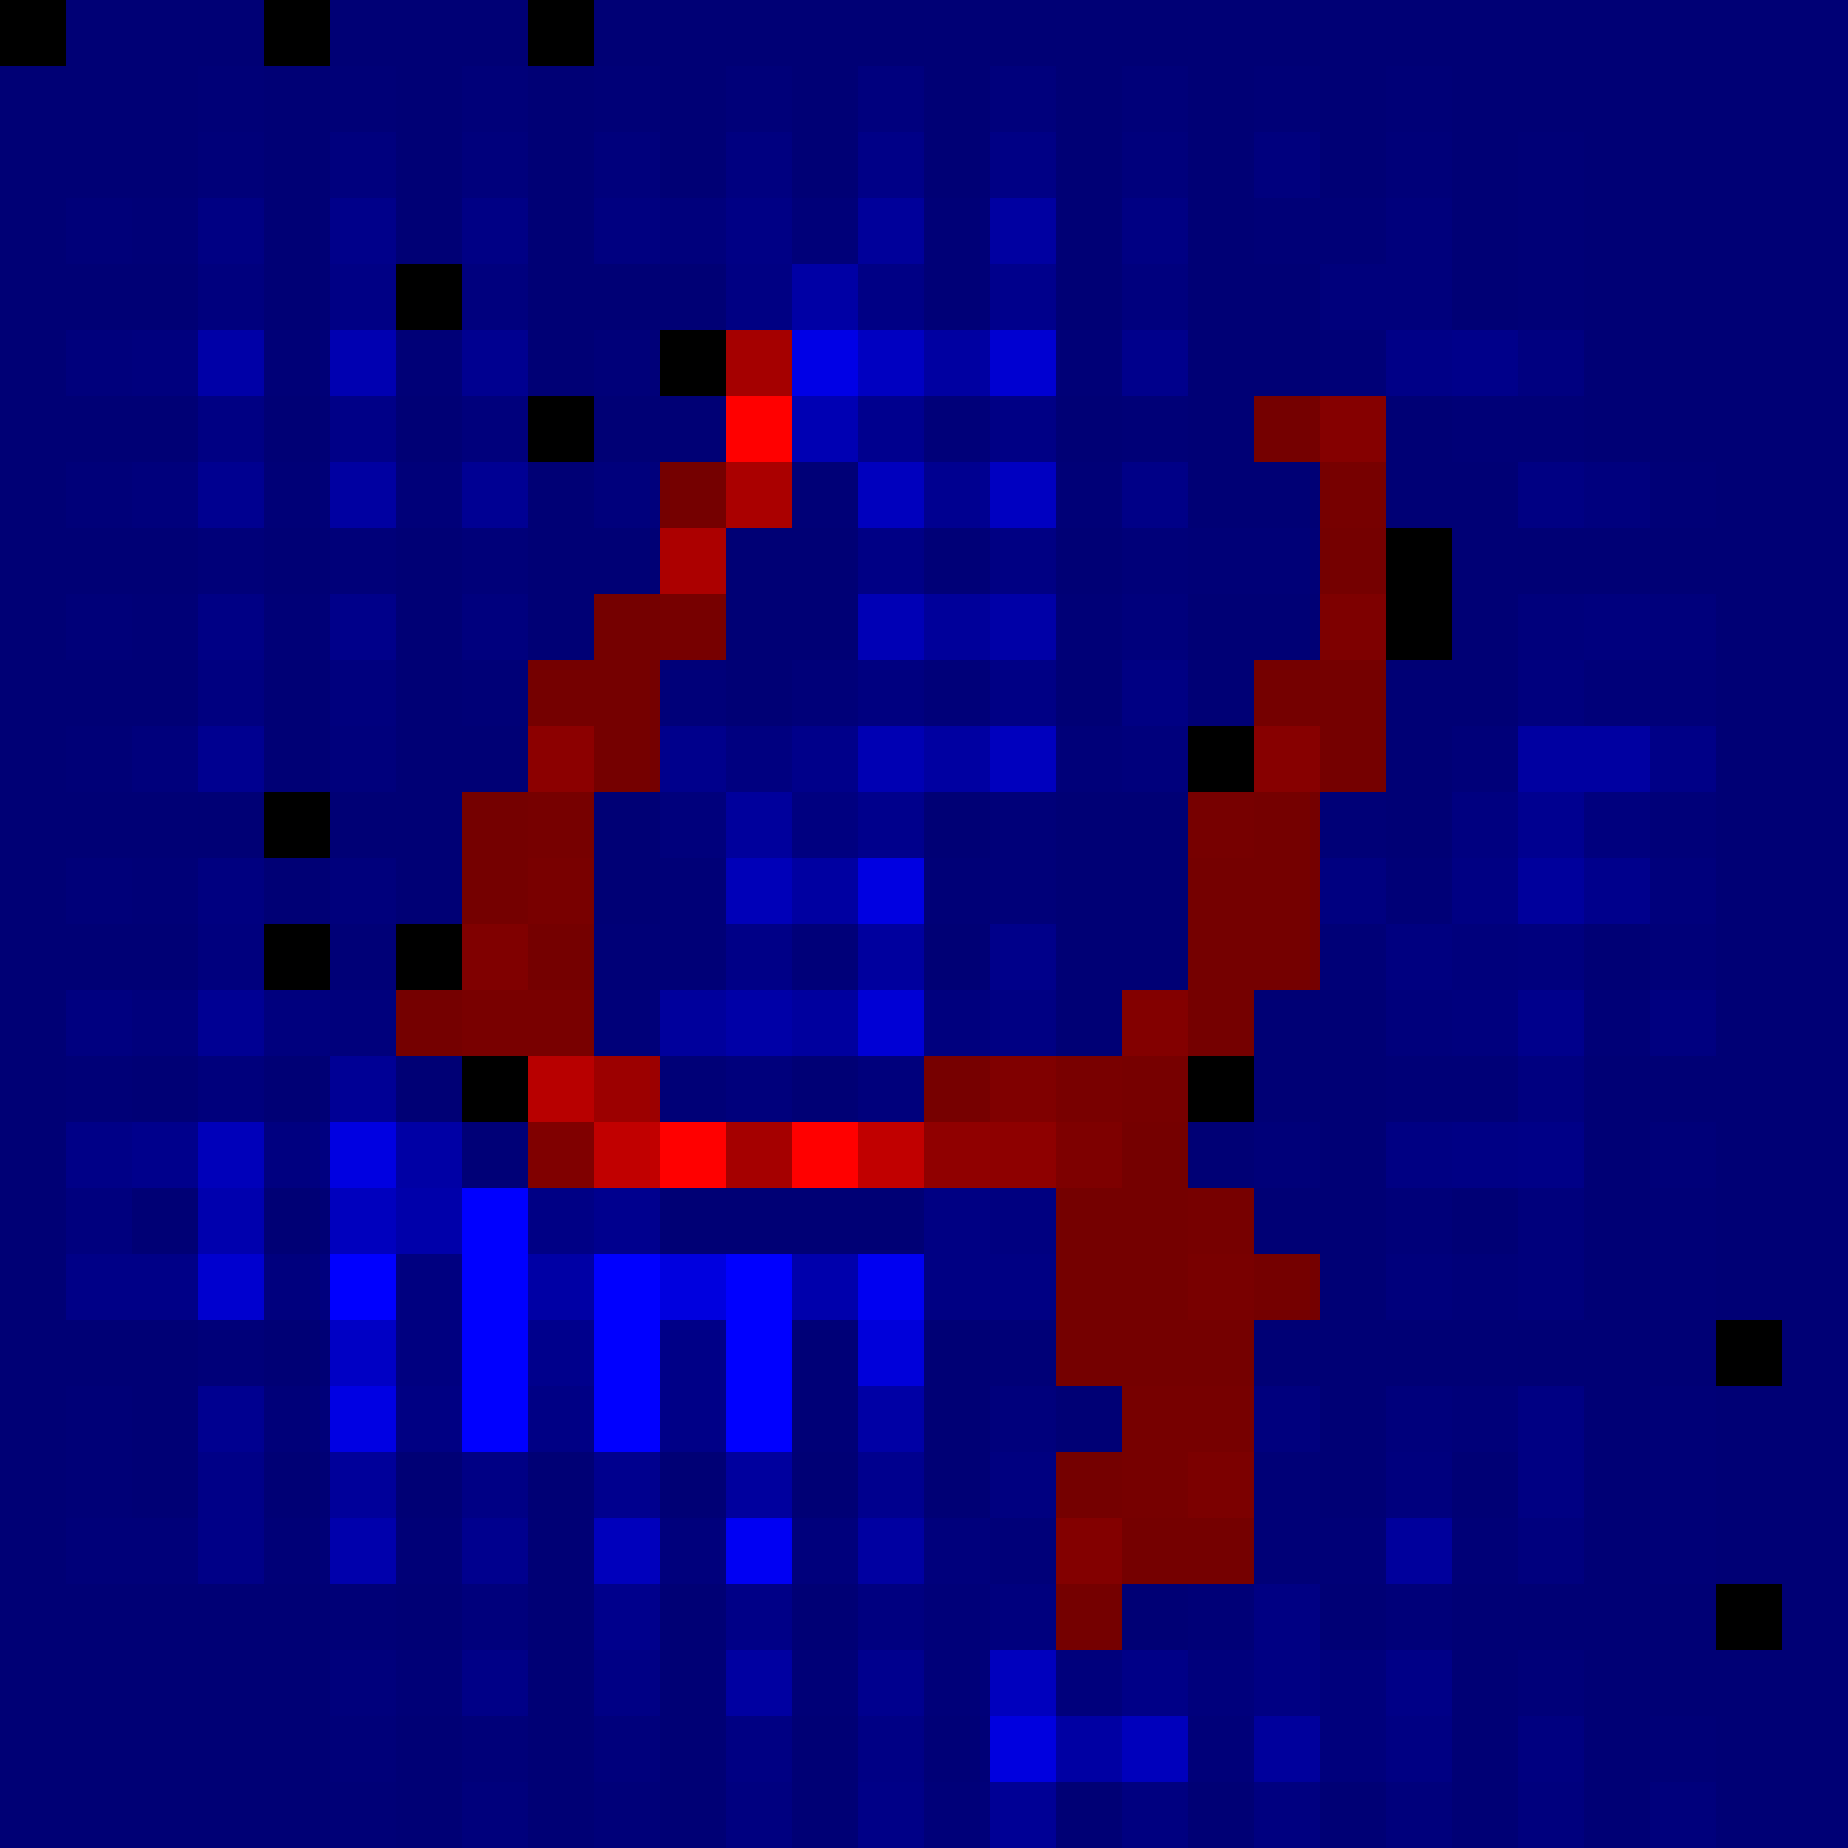
\includegraphics[width=\linewidth]{saliency/mnist_ic_saliency/saliency_threshold_wrt_4_bright.png}
        \scriptsize Gradient 4
    \end{minipage}%
    \begin{minipage}[b]{0.09\linewidth}\centering
        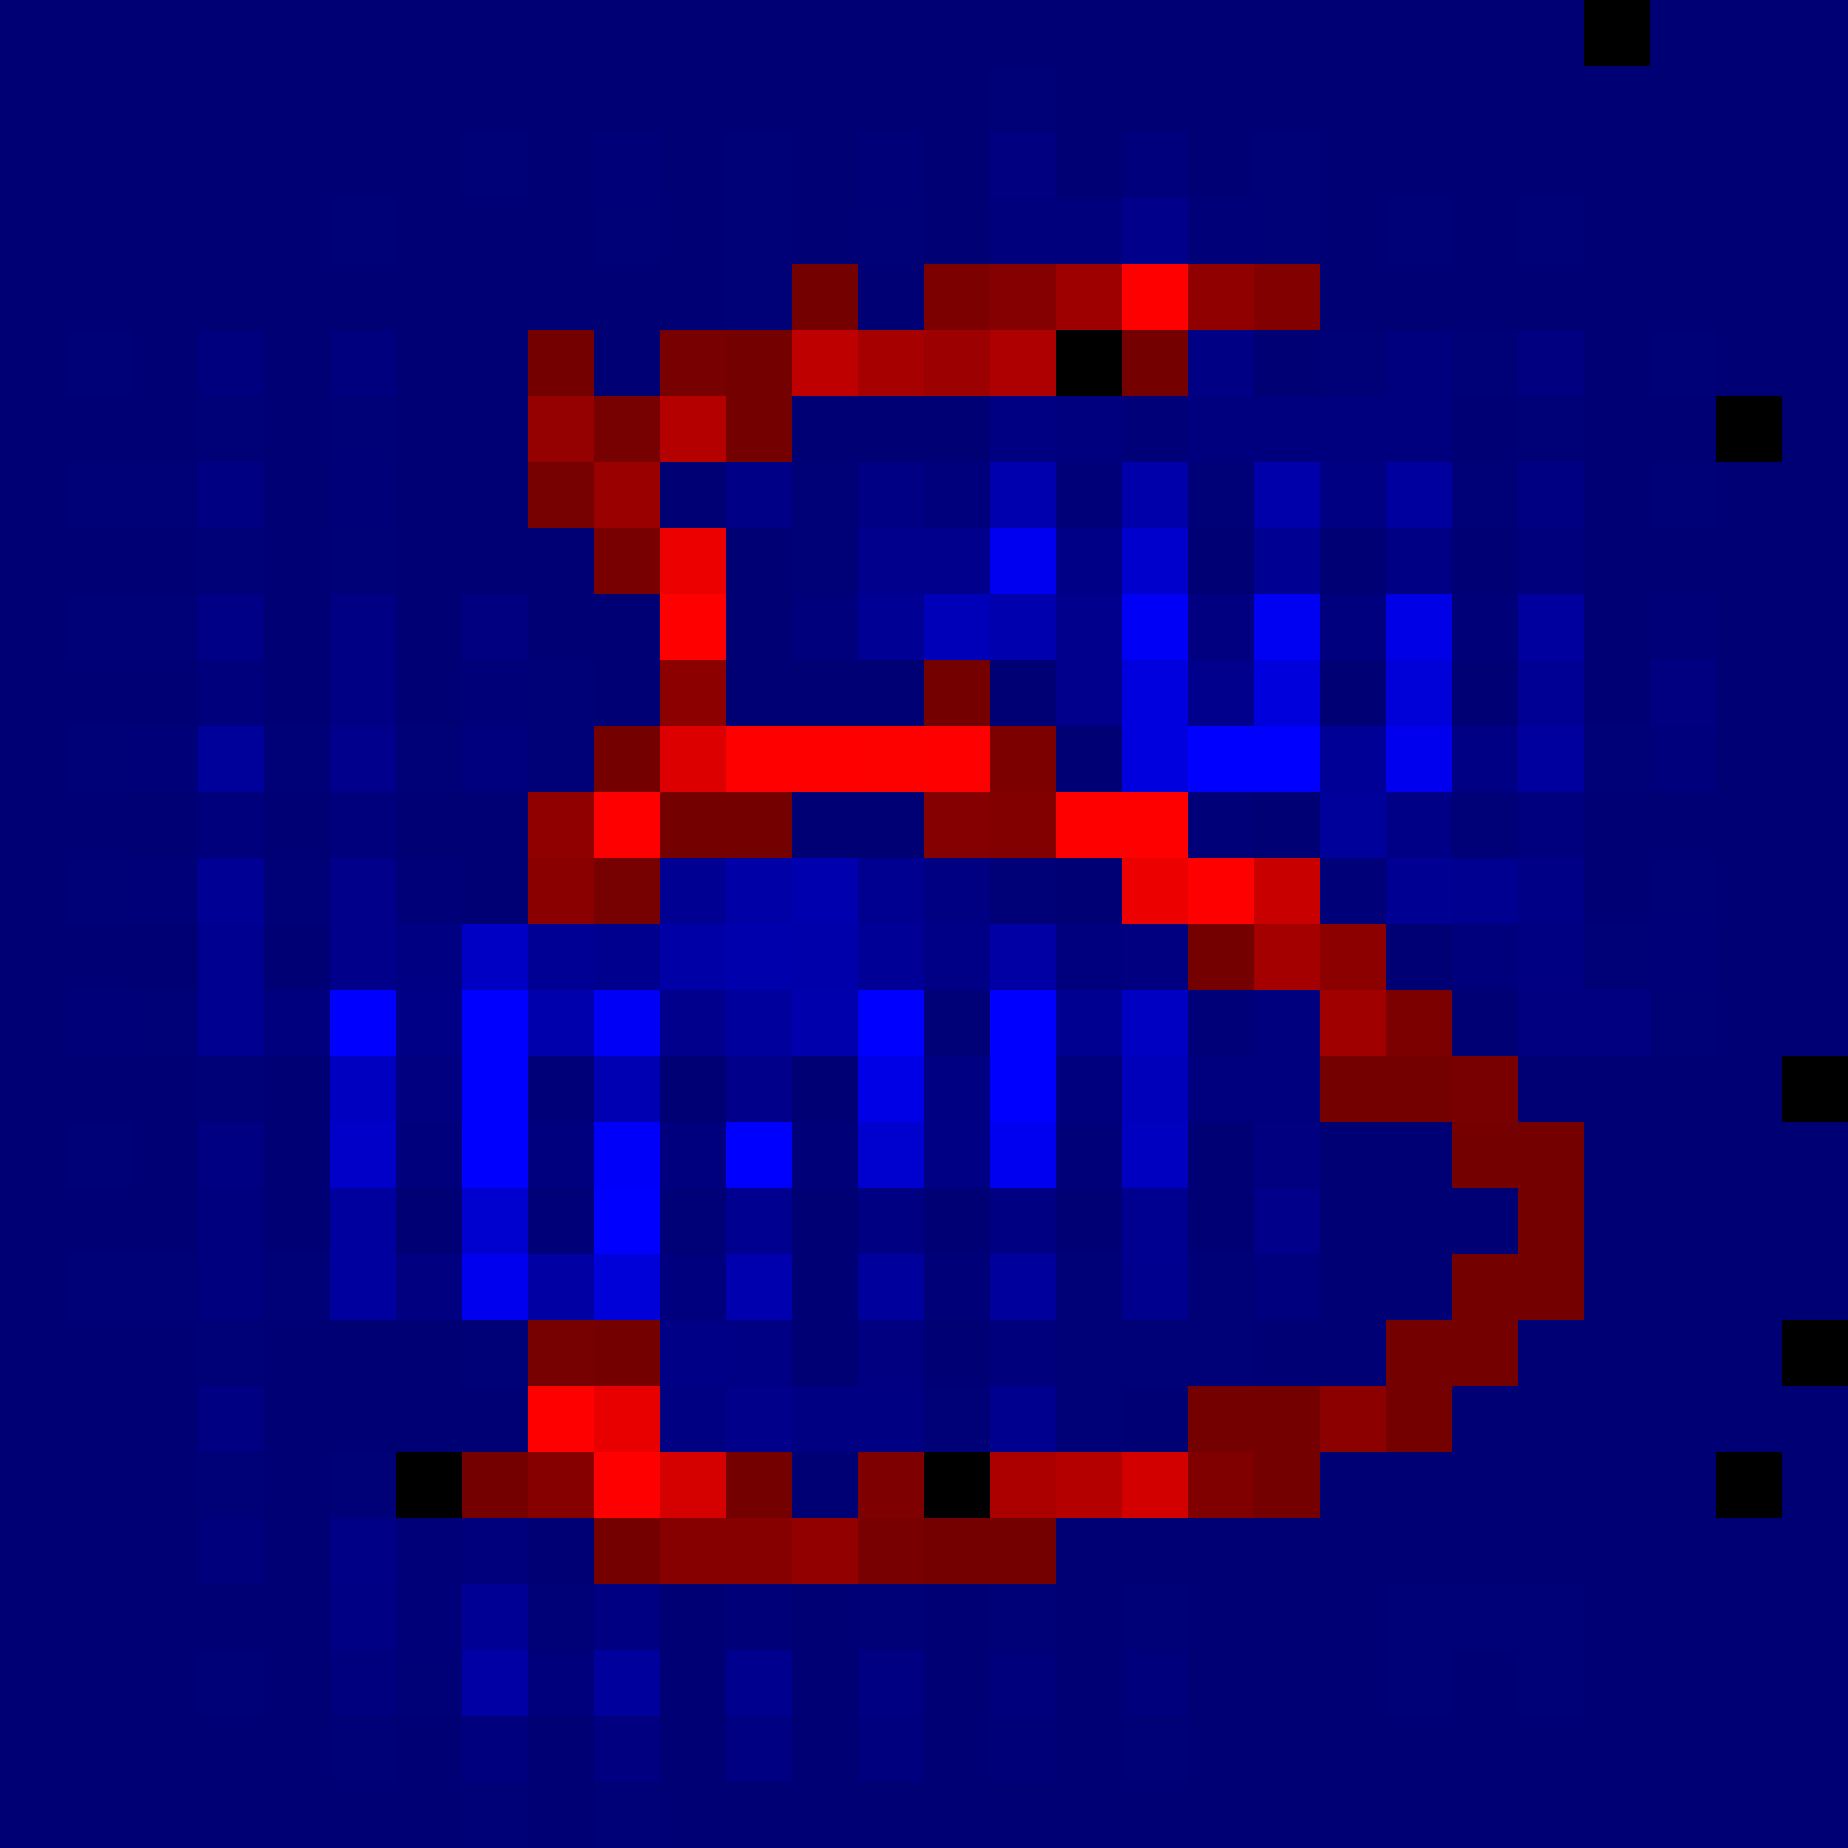
\includegraphics[width=\linewidth]{saliency/mnist_ic_saliency/saliency_threshold_wrt_5_bright.png}
        \scriptsize Gradient 5
    \end{minipage}%
    \begin{minipage}[b]{0.09\linewidth}\centering
        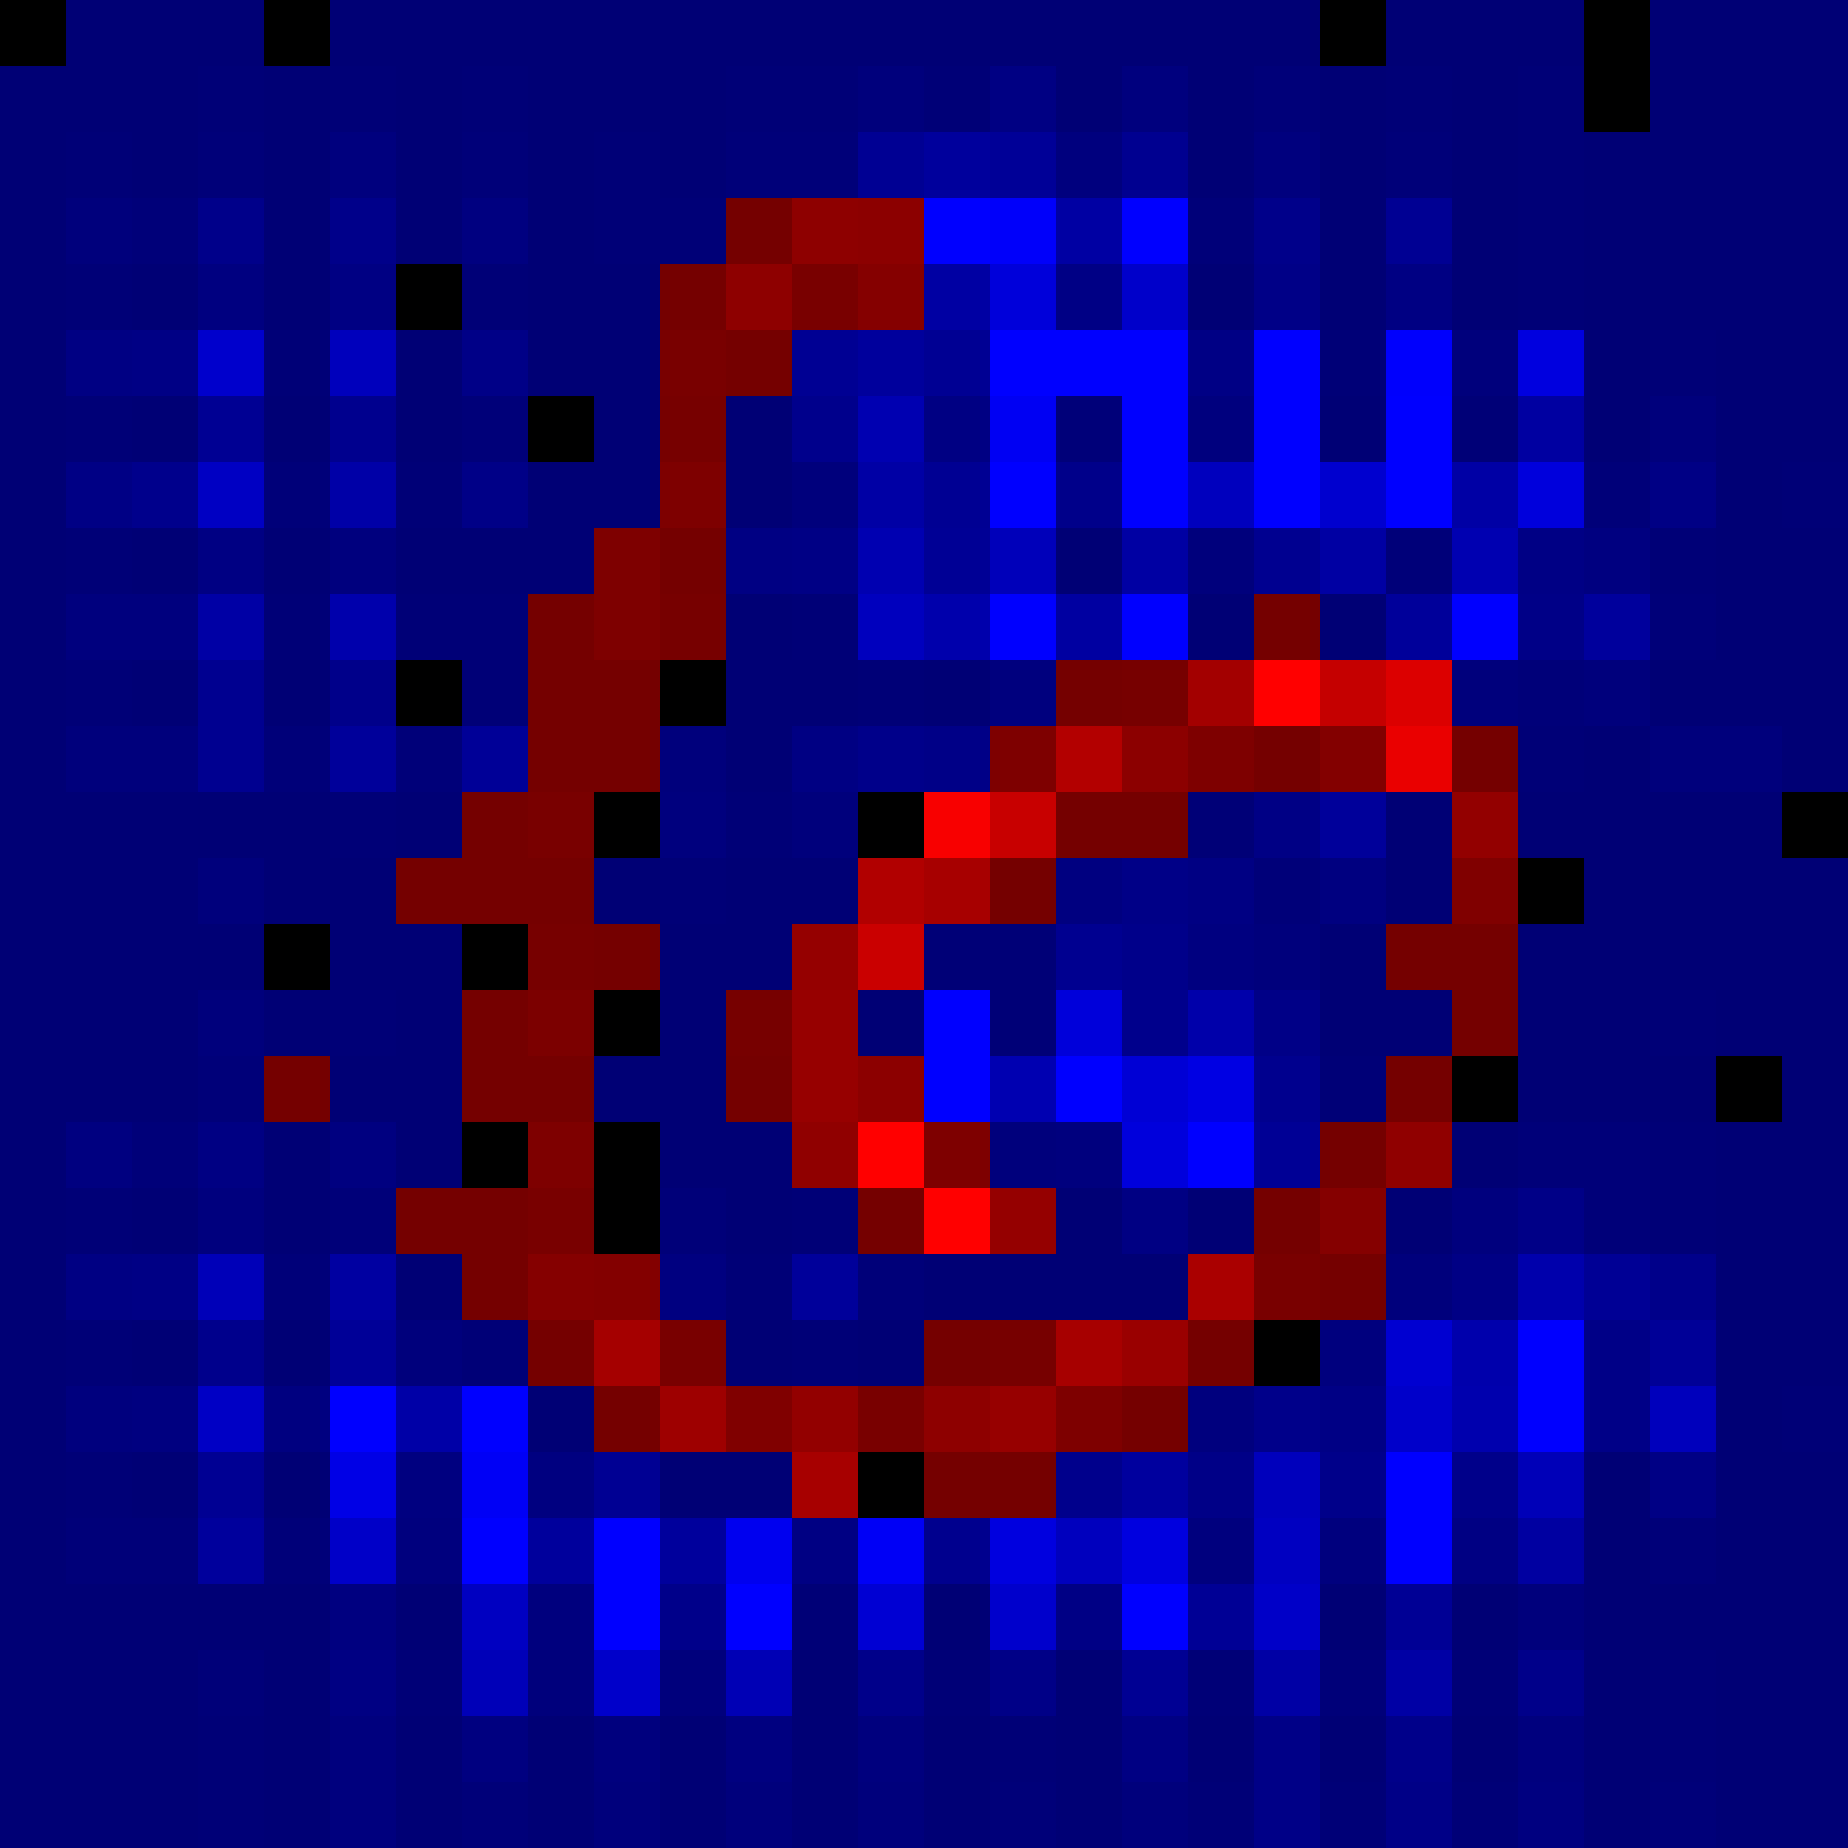
\includegraphics[width=\linewidth]{saliency/mnist_ic_saliency/saliency_threshold_wrt_6_bright.png}
        \scriptsize Gradient 6
    \end{minipage}%
    \begin{minipage}[b]{0.09\linewidth}\centering
        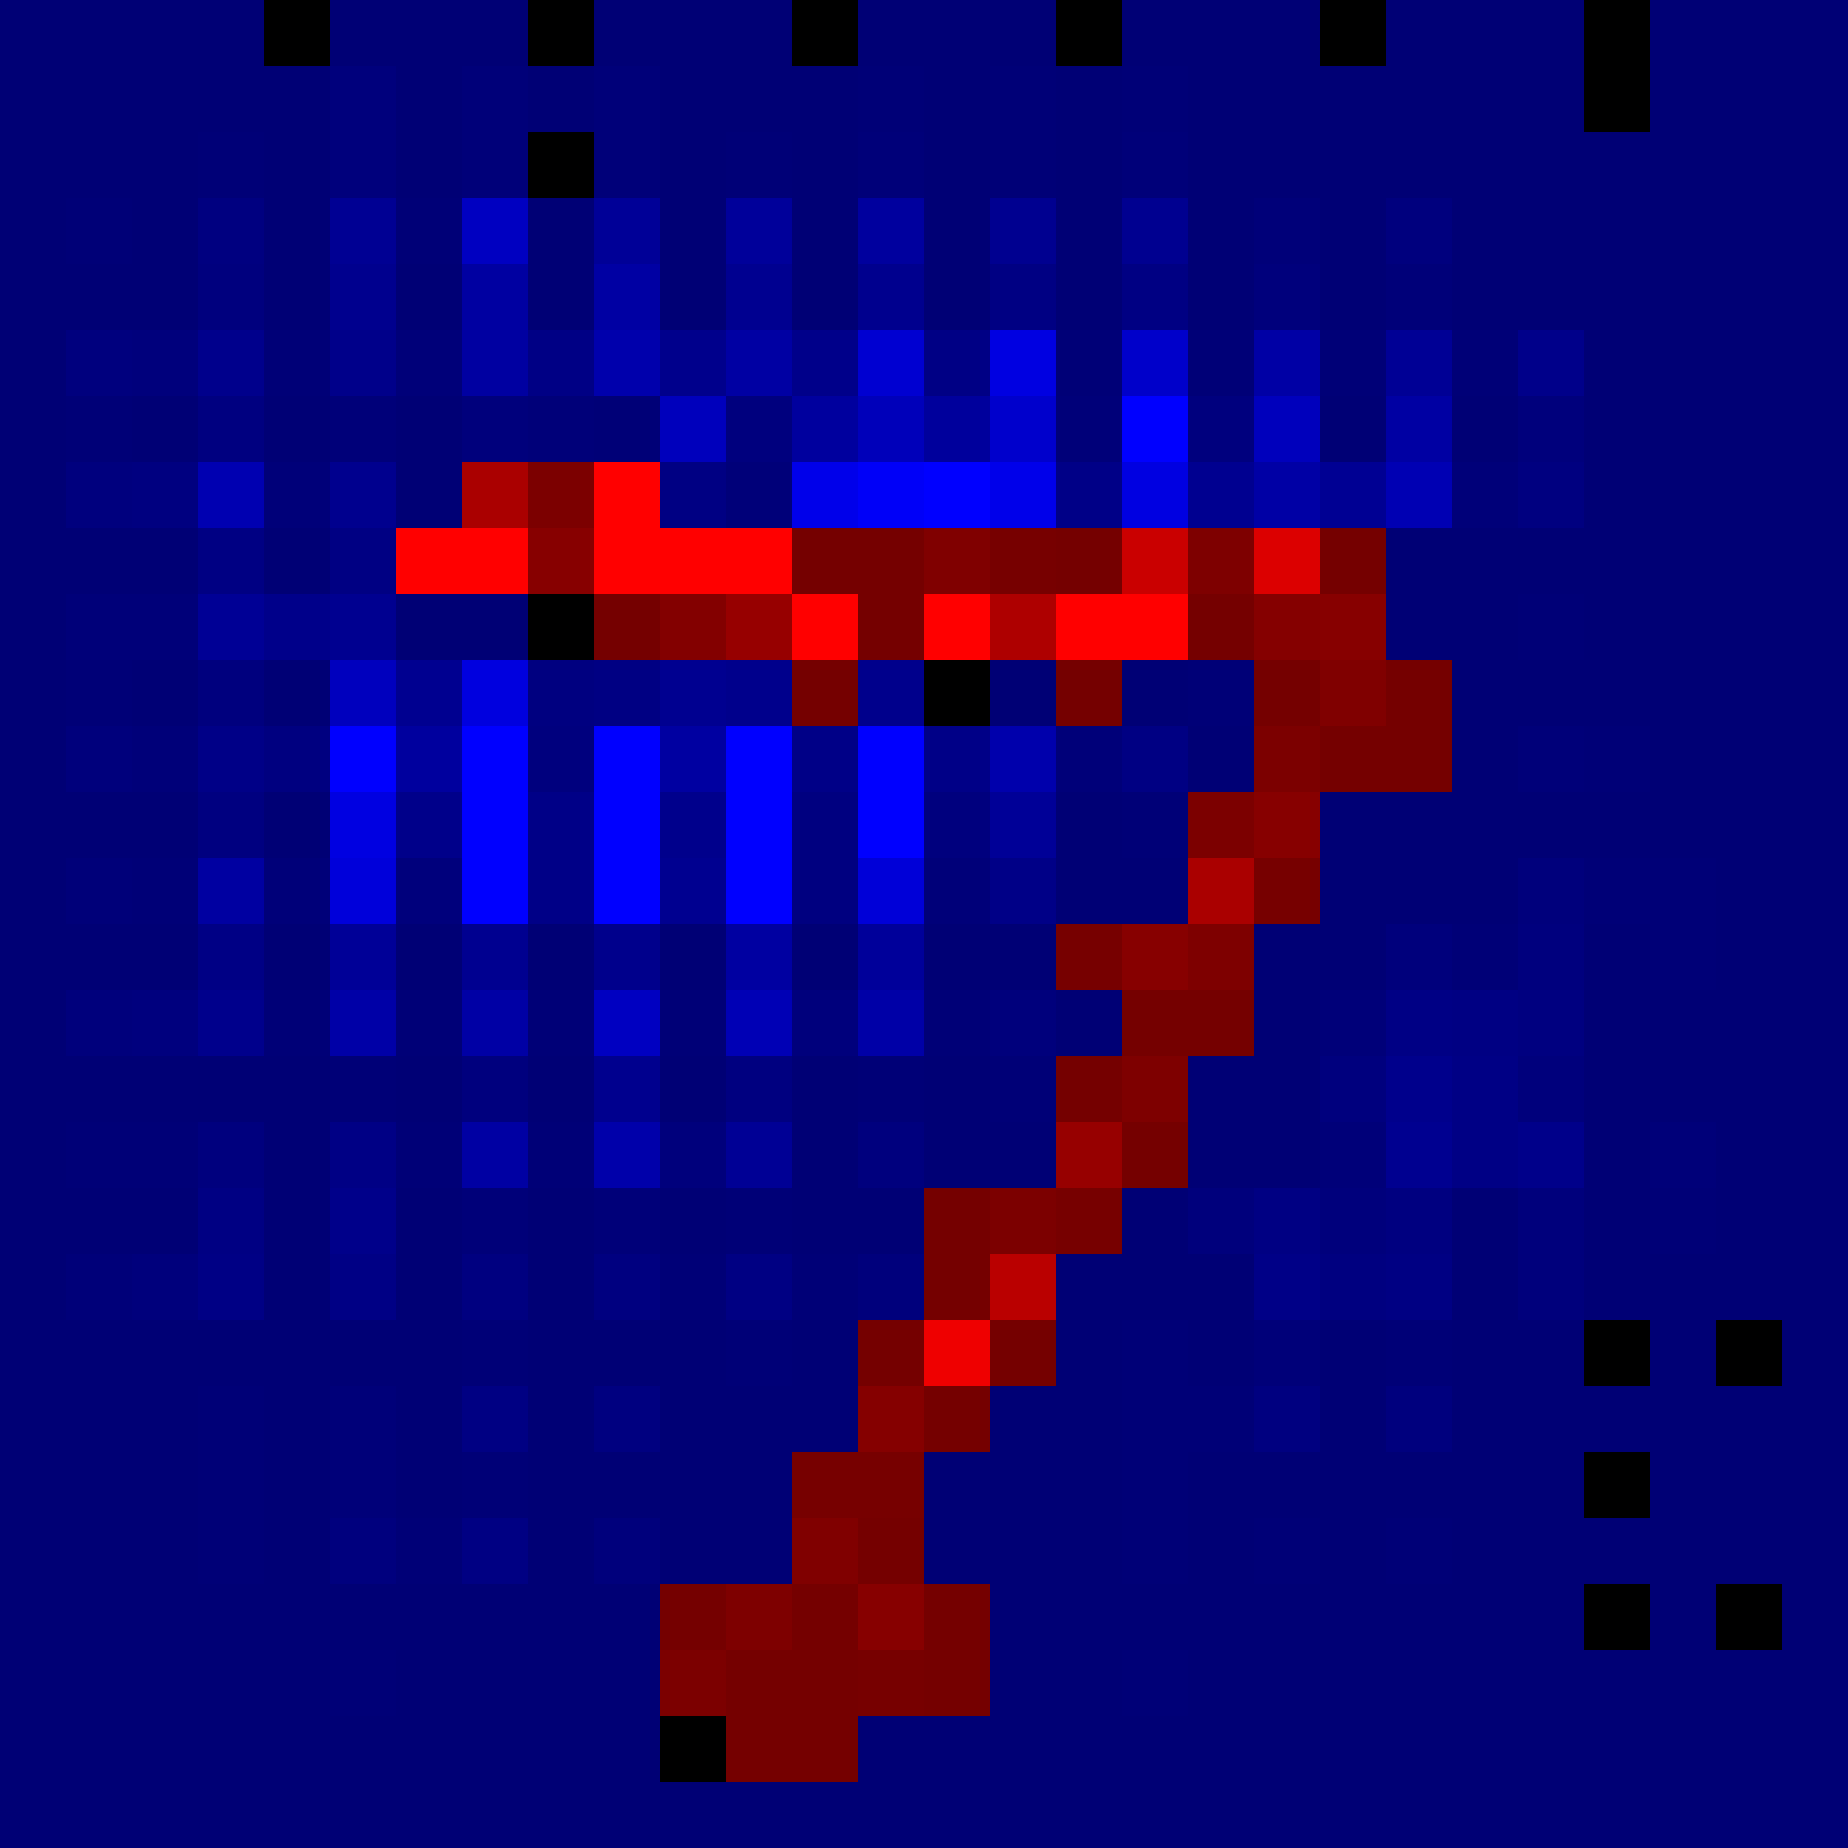
\includegraphics[width=\linewidth]{saliency/mnist_ic_saliency/saliency_threshold_wrt_7_bright.png}
        \scriptsize Gradient 7
    \end{minipage}%
    \begin{minipage}[b]{0.09\linewidth}\centering
        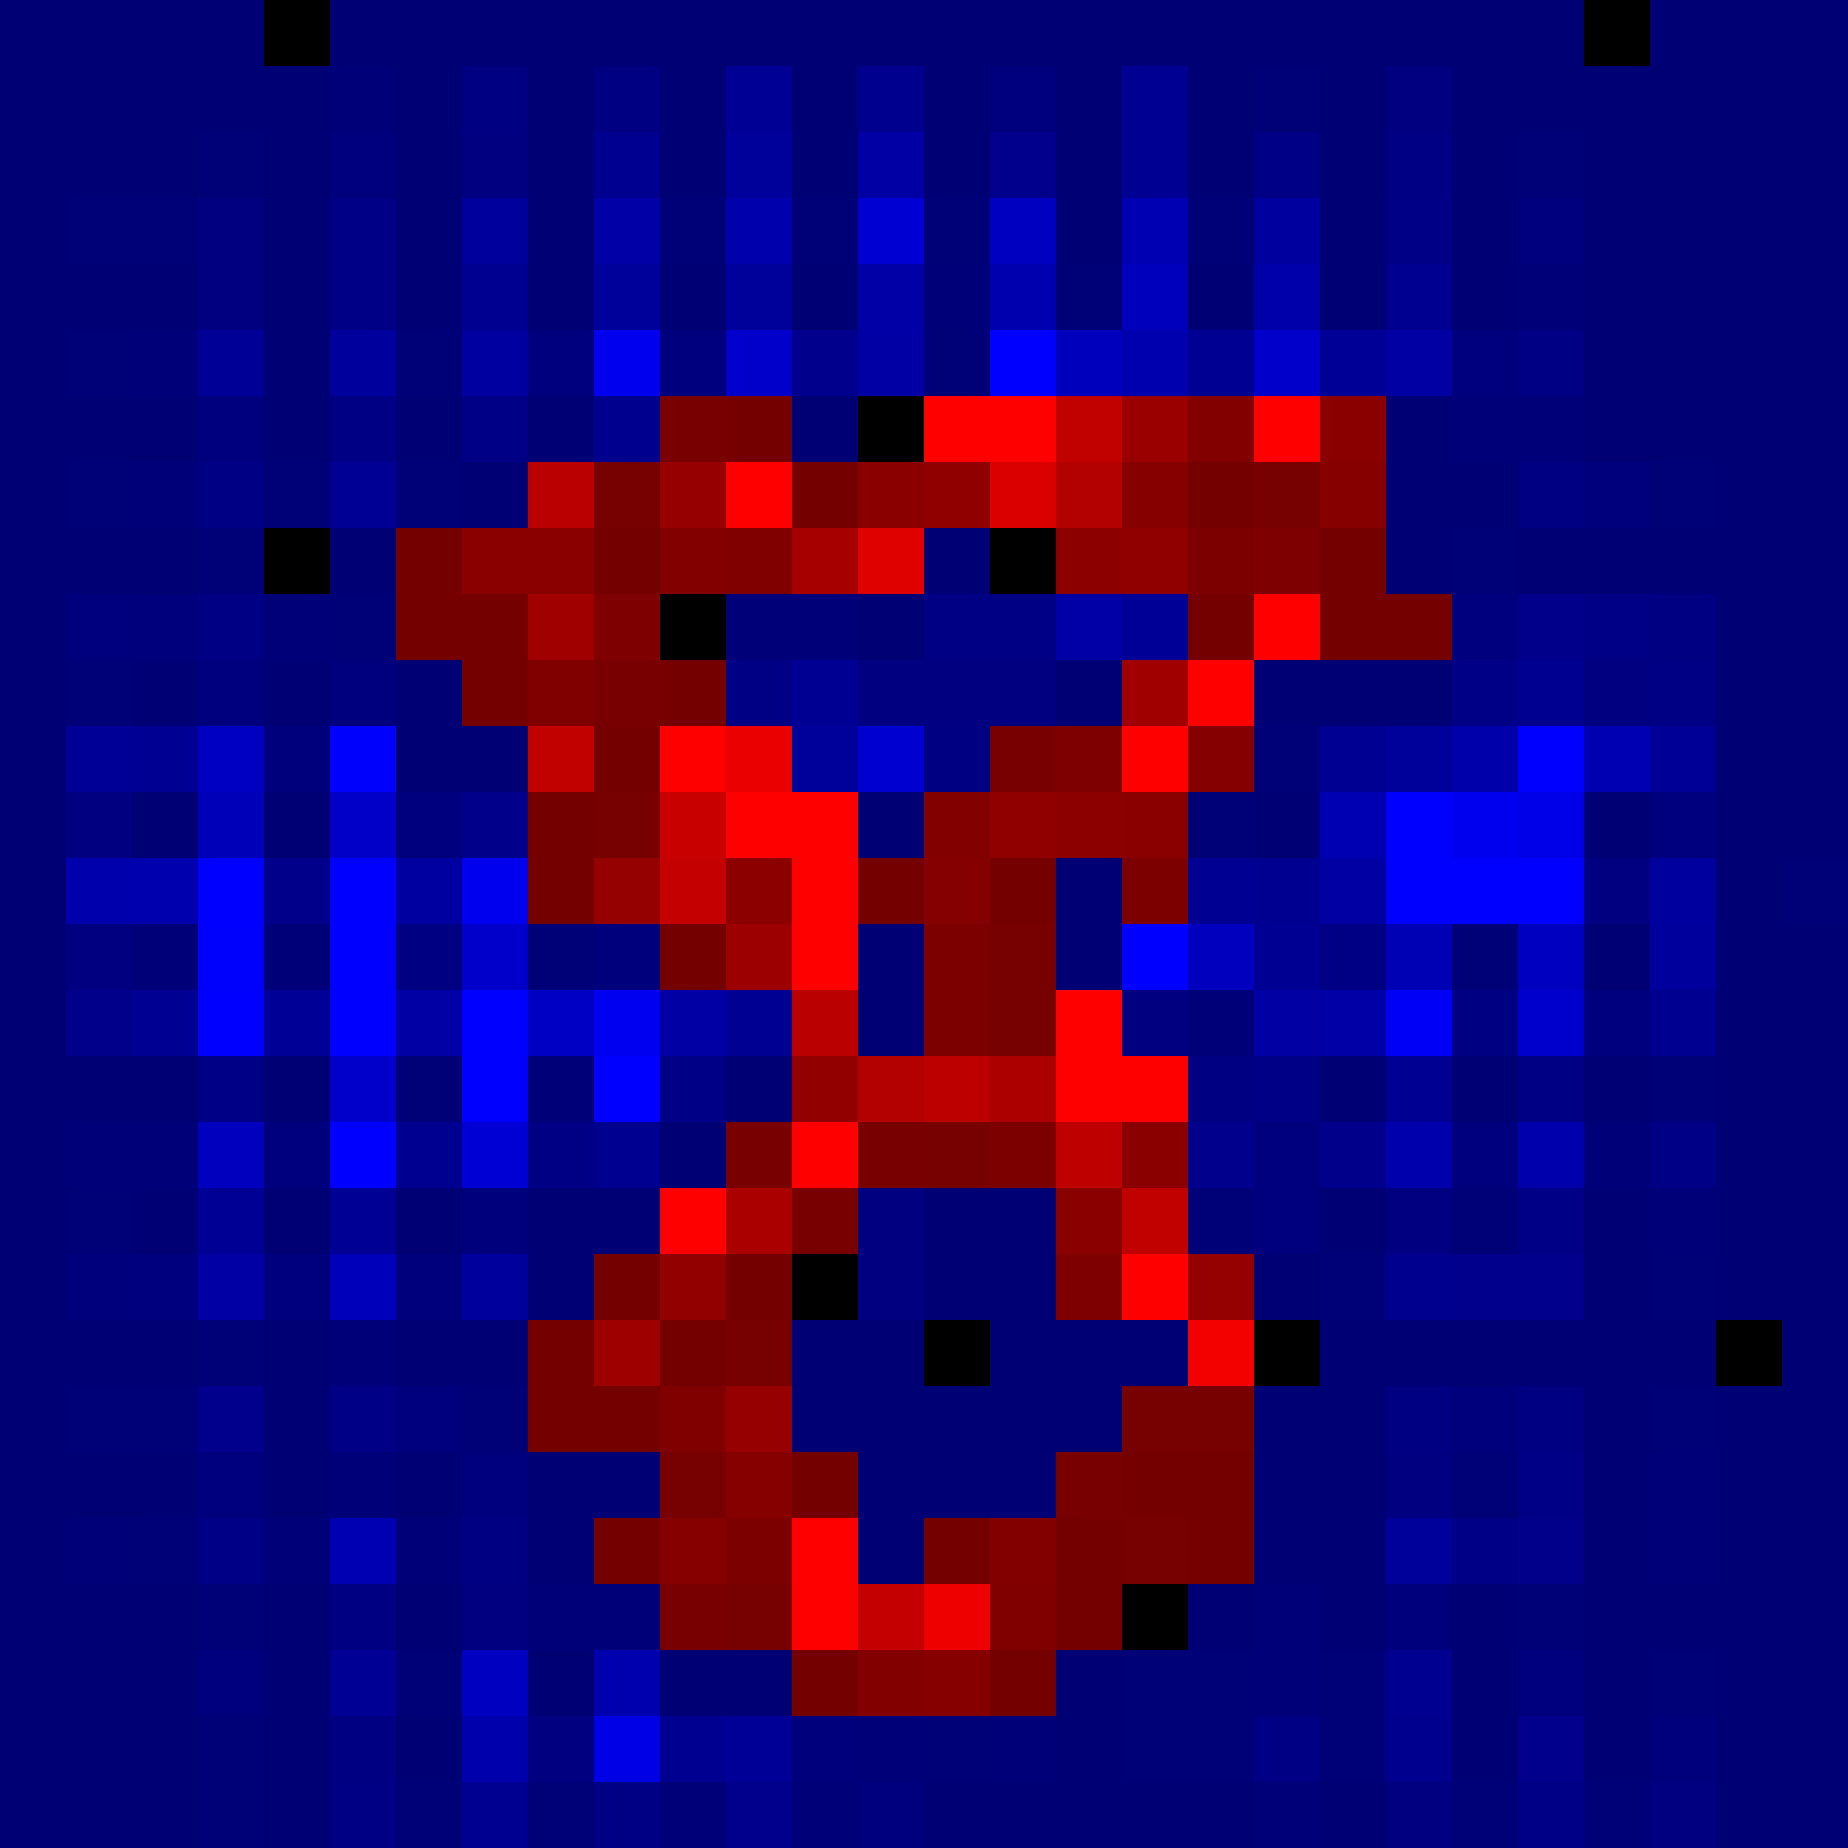
\includegraphics[width=\linewidth]{saliency/mnist_ic_saliency/saliency_threshold_wrt_8_bright.png}
        \scriptsize Gradient 8
    \end{minipage}%
    \begin{minipage}[b]{0.09\linewidth}\centering
        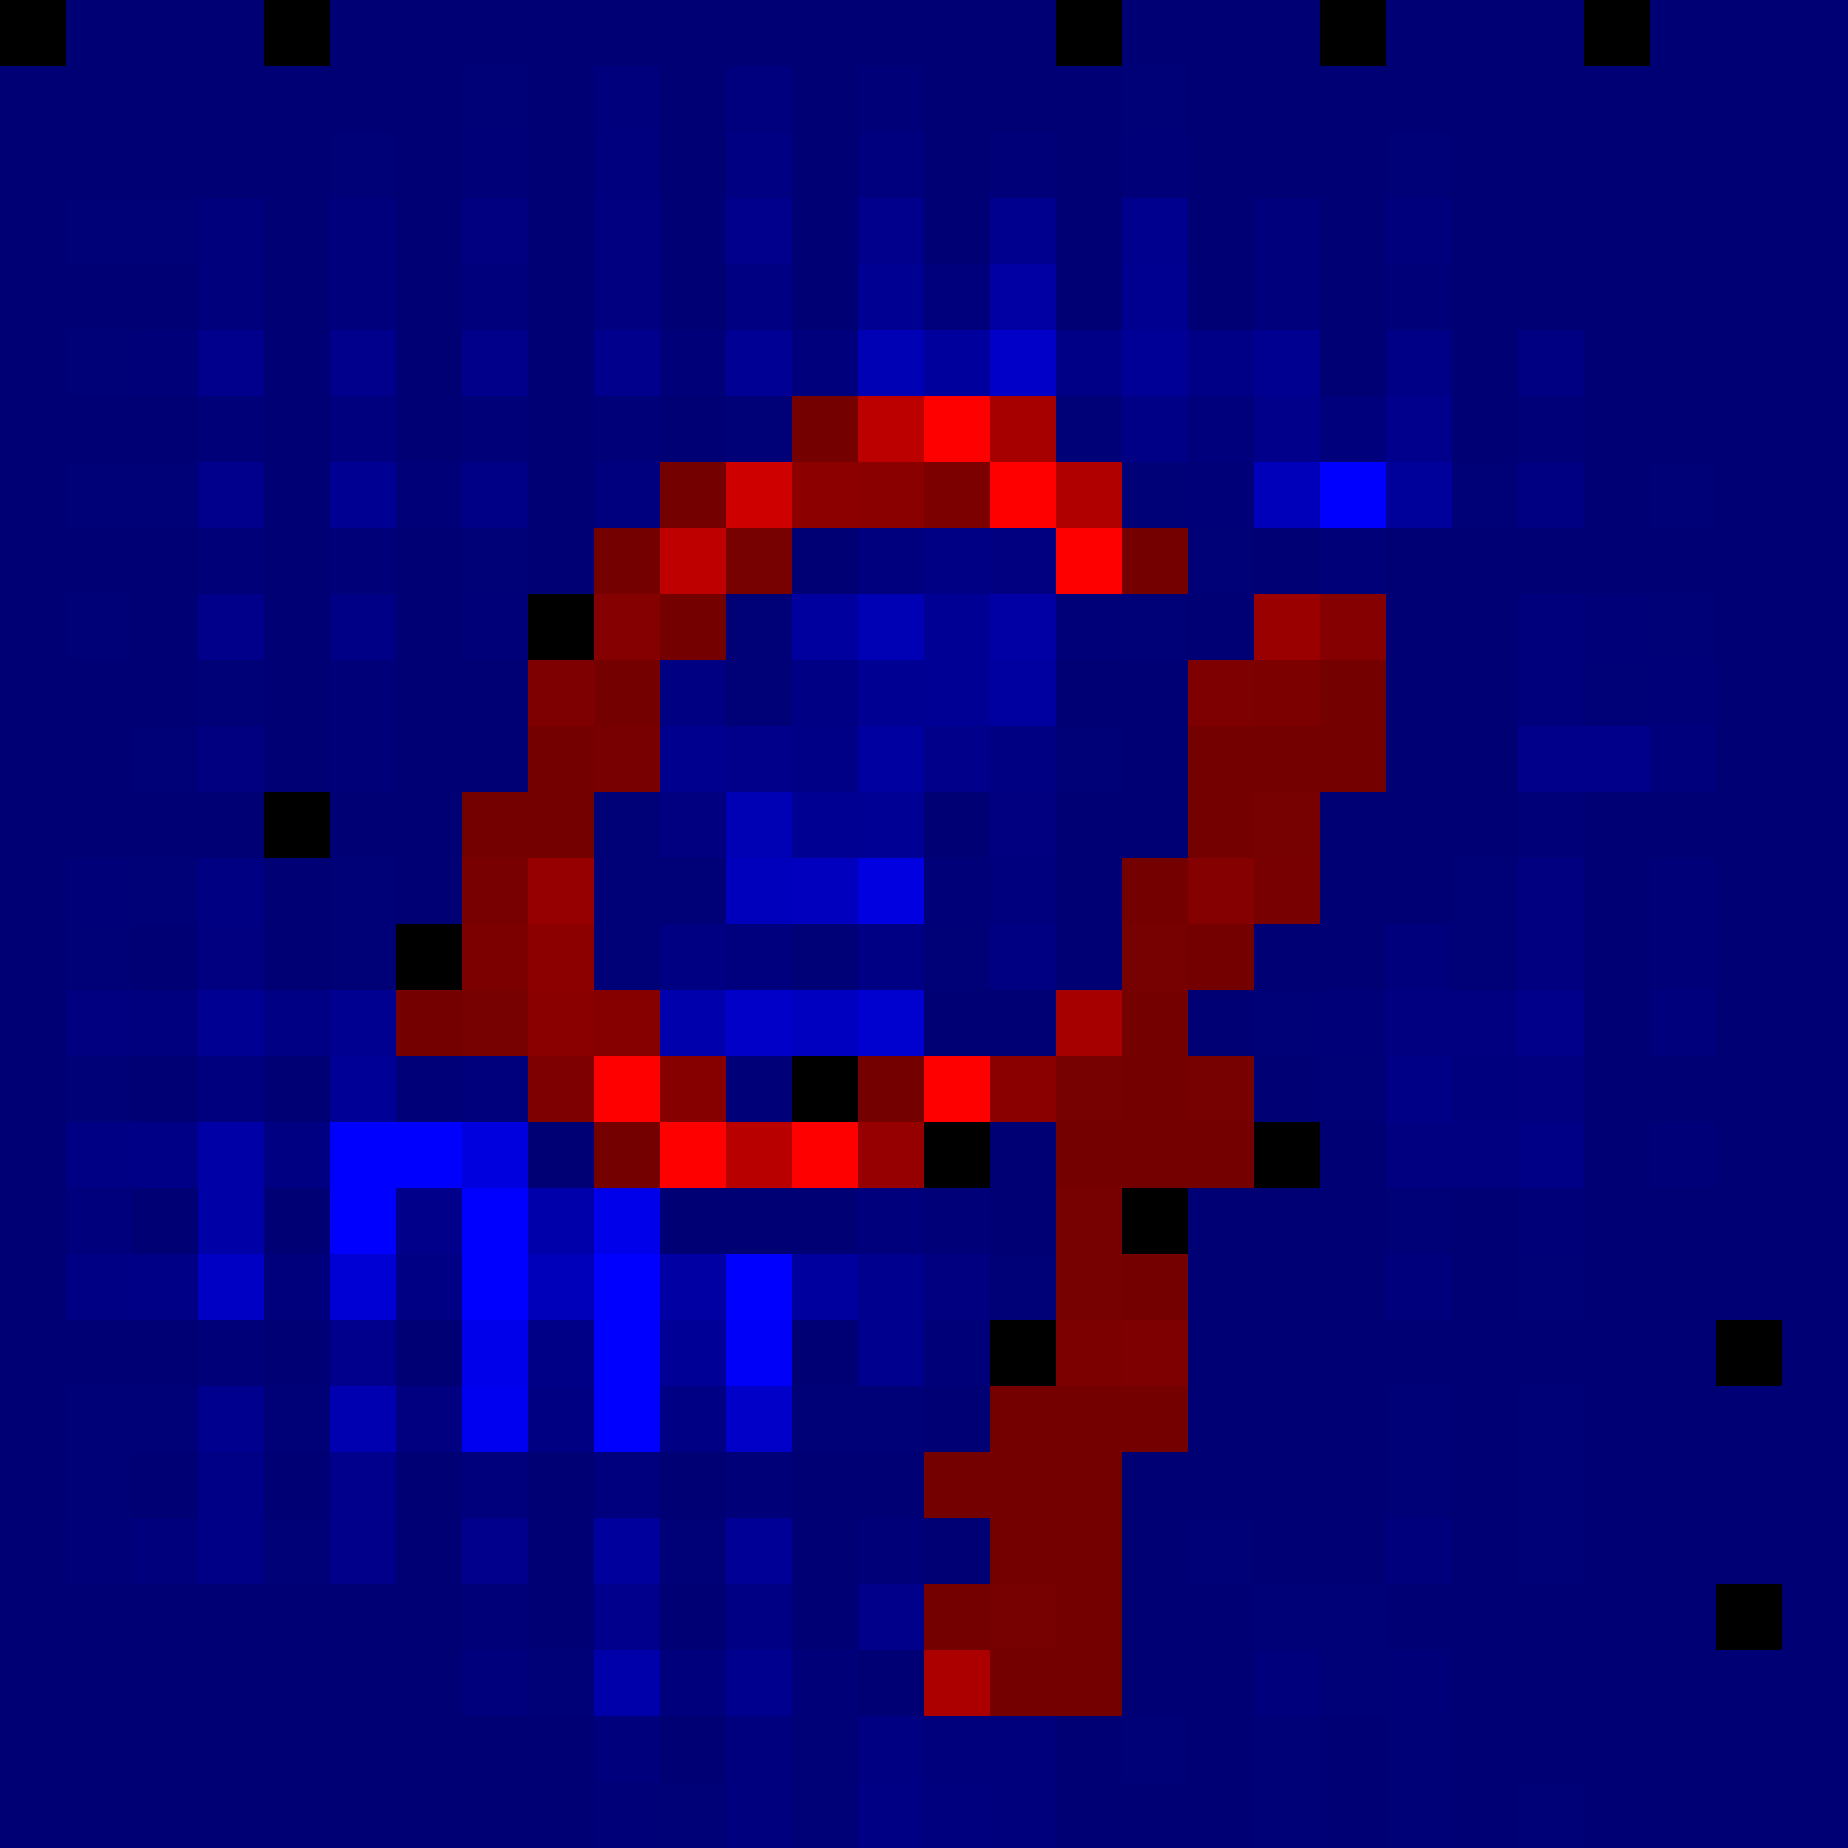
\includegraphics[width=\linewidth]{saliency/mnist_ic_saliency/saliency_threshold_wrt_9_bright.png}
        \scriptsize Gradient 9
    \end{minipage}%

    \par\vspace{0.25cm}
    \begin{minipage}[b]{0.09\linewidth}\centering
        
\includegraphics[width=\linewidth]{saliency/mnist_ic_saliency/original_0.png}
        \scriptsize Label 0
    \end{minipage}%
    \begin{minipage}[b]{0.09\linewidth}\centering
        
\includegraphics[width=\linewidth]{saliency/mnist_ic_saliency/original_1.png}
        \scriptsize Label 1
    \end{minipage}%
    \begin{minipage}[b]{0.09\linewidth}\centering
        
\includegraphics[width=\linewidth]{saliency/mnist_ic_saliency/original_2.png}
        \scriptsize Label 2
    \end{minipage}%
    \begin{minipage}[b]{0.09\linewidth}\centering
        
\includegraphics[width=\linewidth]{saliency/mnist_ic_saliency/original_3.png}
        \scriptsize Label 3
    \end{minipage}%
    \begin{minipage}[b]{0.09\linewidth}\centering
        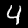
\includegraphics[width=\linewidth]{saliency/mnist_ic_saliency/original_4.png}
        \scriptsize Label 4
    \end{minipage}%
    \begin{minipage}[b]{0.09\linewidth}\centering
        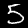
\includegraphics[width=\linewidth]{saliency/mnist_ic_saliency/original_5.png}
        \scriptsize Label 5
    \end{minipage}%
    \begin{minipage}[b]{0.09\linewidth}\centering
        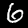
\includegraphics[width=\linewidth]{saliency/mnist_ic_saliency/original_6.png}
        \scriptsize Label 6
    \end{minipage}%
    \begin{minipage}[b]{0.09\linewidth}\centering
        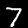
\includegraphics[width=\linewidth]{saliency/mnist_ic_saliency/original_7.png}
        \scriptsize Label 7
    \end{minipage}%
    \begin{minipage}[b]{0.09\linewidth}\centering
        
\includegraphics[width=\linewidth]{saliency/mnist_ic_saliency/original_8.png}
        \scriptsize Label 8
    \end{minipage}%
    \begin{minipage}[b]{0.09\linewidth}\centering
        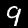
\includegraphics[width=\linewidth]{saliency/mnist_ic_saliency/original_9.png}
        \scriptsize Label 9
    \end{minipage}%

    }%
\caption[Input-gradient visualizations for ten MNIST digits]{Input-gradient visualizations of the \texttt{cnn\_maxout} IC model for ten MNIST digits, each with respect to its ground-truth label. Top: saliency maps; bottom: input images. As in the source figure, positive and negative gradient values above threshold 0.2 are colored red and blue, with ranking colorized using exponential decay.}
    \label{fig:mnist_ic_saliency}
\end{figure}


\paragraph{Accuracy trade-offs.}\label{subsec:dcinn_accuracy}

Architectural constraints can reduce expressivity~\parencite{Sill1997_MonotonicNetworks,Liu2020CertifiedMonotone}, but for the difference-of-two construction the accuracy cost is small on the convolutional base model and even negative on the \ac{mlp}, where every difference-of-two variant outperforms the unconstrained baseline; the full accuracy table across ten seeds and all eight variants is reported in Chapter~\ref{ch:experiments}.

\begin{remark}[Post-hoc and by-design, reconciled]\label{rem:posthoc_bydesign}
The MNIST study probes the same opposing-stream mechanism as post hoc decomposition: directly trained differences reach competitive accuracy and show class-dependent sensitivities on present and candidate missing strokes. Establishing faithful counterfactuals or general explanatory-role separation for these models and pretrained VGG-16/ResNet-18 split-pairs requires complete-model interventions and larger-architecture tests (Chapter~\ref{ch:conclusion}).
\end{remark}

\section{Game-Based Attribution: Modes and Technicalities}\label{sec:game_based_attribution}

The game route attributes by the per-neuron difference of players' discounted equilibrium occupation measures. It recovers gradients in the \ac{sg} (Theorem~\ref{ptnb:thm:gradient}) and the full $\alpha\beta$-\ac{lrp} family in the \ac{rg} at $\tau=1$ (Theorem~\ref{thm:lrp_recovery}). Here we collect tunable \emph{modes} and input-side \emph{technicalities}.

\subsection{Attribution Modes}\label{subsec:attribution_modes}

Chapter~\ref{ch:game_theory} varies equilibrium trajectory laws through routing and stopping temperatures $\tau,\theta$, the policy-entropy bonus, risk $\lambda\le0$, stream balance $(\alpha,\beta)$, and \ac{lrp} stabilization $\epsilon\ge0$. Section~\ref{sec:risk_aversion_regularization} gives an exact dictionary from each parameter to its backward rule. These controls yield tunable attribution maps and form the sweeps of Chapter~\ref{ch:experiments}.

Here $(\alpha,\beta)$ denotes the $\alpha\beta$-\ac{lrp} discount pair, with $\alpha-\beta=1$ and anchor $(2,1)$ weighting support against opposition; a bare $\alpha$ is this stream weight, unrelated to the backward shift $\alpha\in[0,\tfrac12]$ of Section~\ref{sec:split_attribution_concept}. Routing temperature $\tau$ recovers $\alpha\beta$-\ac{lrp} exactly only at $\tau=1$ (Theorem~\ref{thm:lrp_recovery}); its myopic application preserves the forward pass. It is distinct from the spatial transforms $\tau_t$ below.

\subsection{Technicalities}\label{subsec:technicalities}

Input-transform averaging and a detached-operator (DAVE-style) reading of the gradient decomposition improve maps without changing the game. They matter especially for \acp{vit}, whose $16\times16$ patch tokenization breaks translation equivariance and introduces grid artifacts~\parencite{Wrobel2024,Dosovitskiy2021vit}.

\paragraph{Reynolds-inspired averaging.} Following DAVE~\parencite{Wrobel2024}, compute attributions on $N$ randomly transformed inputs (small rotations, translations, horizontal flips), map them back by $\tau_t^{-1}$, and average. These spatial transforms $\tau_1,\dots,\tau_N$ are distinct from routing temperature $\tau$. Reynolds-inspired averaging can suppress transform-dependent architectural artifacts while retaining common image structure; $N$ trades computation for smoothness and is ablated in Chapter~\ref{ch:experiments}.

\paragraph{Connection to DAVE-style gradient decomposition.} The averaging pairs with a \emph{conditioned forward pass} inspired by DAVE \parencite{Wrobel2024}. Our game fixes both LayerNorm statistics, the GELU gate and the softmax row; DAVE retains linear mean-centering while fixing the normalization scale. Conservation concerns the game's propagation rule with its bias accounting. The attribution takes the transform-averaged input$\times$gradient form $\tfrac{1}{N}\sum_t \tau_t^{-1}(W_t) \odot X$, where $W_t$ is the conditioned backward signal on the $t$-th transformed input. Chapter~\ref{ch:transformers} specifies the conditioned operators used by the game-based maps.
